\begin{savequote}[75mm]
In god we trust. 
All others bring data. 
\qauthor{William Edwards Demming (1900-1993)}
\end{savequote}

\chapter{Case Study Results}
\label{Chapter 4}

\newpage

\section{Santa Barbara Region}

The first case study region, comprising the coastal southern portion of Santa Barbara County, was selected to reflect the local interests of the institution supporting this dissertation research. Hydrologically, this case study region is distinctly enclosed by a steep coastal mountain range to the north and the pacific ocean to the south. This case study area is not connected to any of the major inter-basin water transfer projects within the state (i.e. The State Water Project, the Los Angeles aqueduct, etc.). As such, Santa Barbara municipal water managers must be both creative and self reliant in terms of their long term municipal water supply strategies. 

Fortunately, from a freshwater management perspective, the region's unique physical geography also functions to limit the possibilities for increased population growth and urban development. Thus, the prospects for severe water shortages due to steep increases in demand are fairly unlikely. Despite this fact however, the recent drought condition throughout the state have lead to high wholesale water costs for the Santa Barbara district. This is because they are in competition with regional agricultural interests with long term investments in costly orchard based crops that cannot be left to fallow. 

In terms of alternative water supply options within the region, Santa Barbara has recently renewed talks for the development of a local seawater desalination plant that had been put on hold following the 2008 economic recession. This willingness to reconsider a high cost desalination based alternative freshwater supply strategy suggests that large scale municipal water reuse may also be put forth as a feasible alternative in the near term future and thus, that such a prospective analysis of the tradeoffs associated with such a system would indeed be valuable exercise.  

    \subsection{Regional Context}
    
    \begin{itemize}
      \setlength{\itemsep}{0cm}
      \setlength{\parskip}{0cm}
        \item HUC-8 Code: $18060013$
        \item Total Area: $1,173.6$ $km^2$
        \item Maximum Elevation: $1,376.7$ $m$
        \item Minimum Elevation: $-0.7$ $m$
        \item Mean Slope: $13.98$ $\%$
        \item Standard Deviation of Slope: $11.07$ $\%$
        \item Dominant Soil Composition: Hydrologic Soil Group - B: $10-20\%$ clay, $50-90\%$ sand, $35\%$ rock fragments
    \end{itemize}
    
        \begin{figure}[!h]
            \begin{center}
            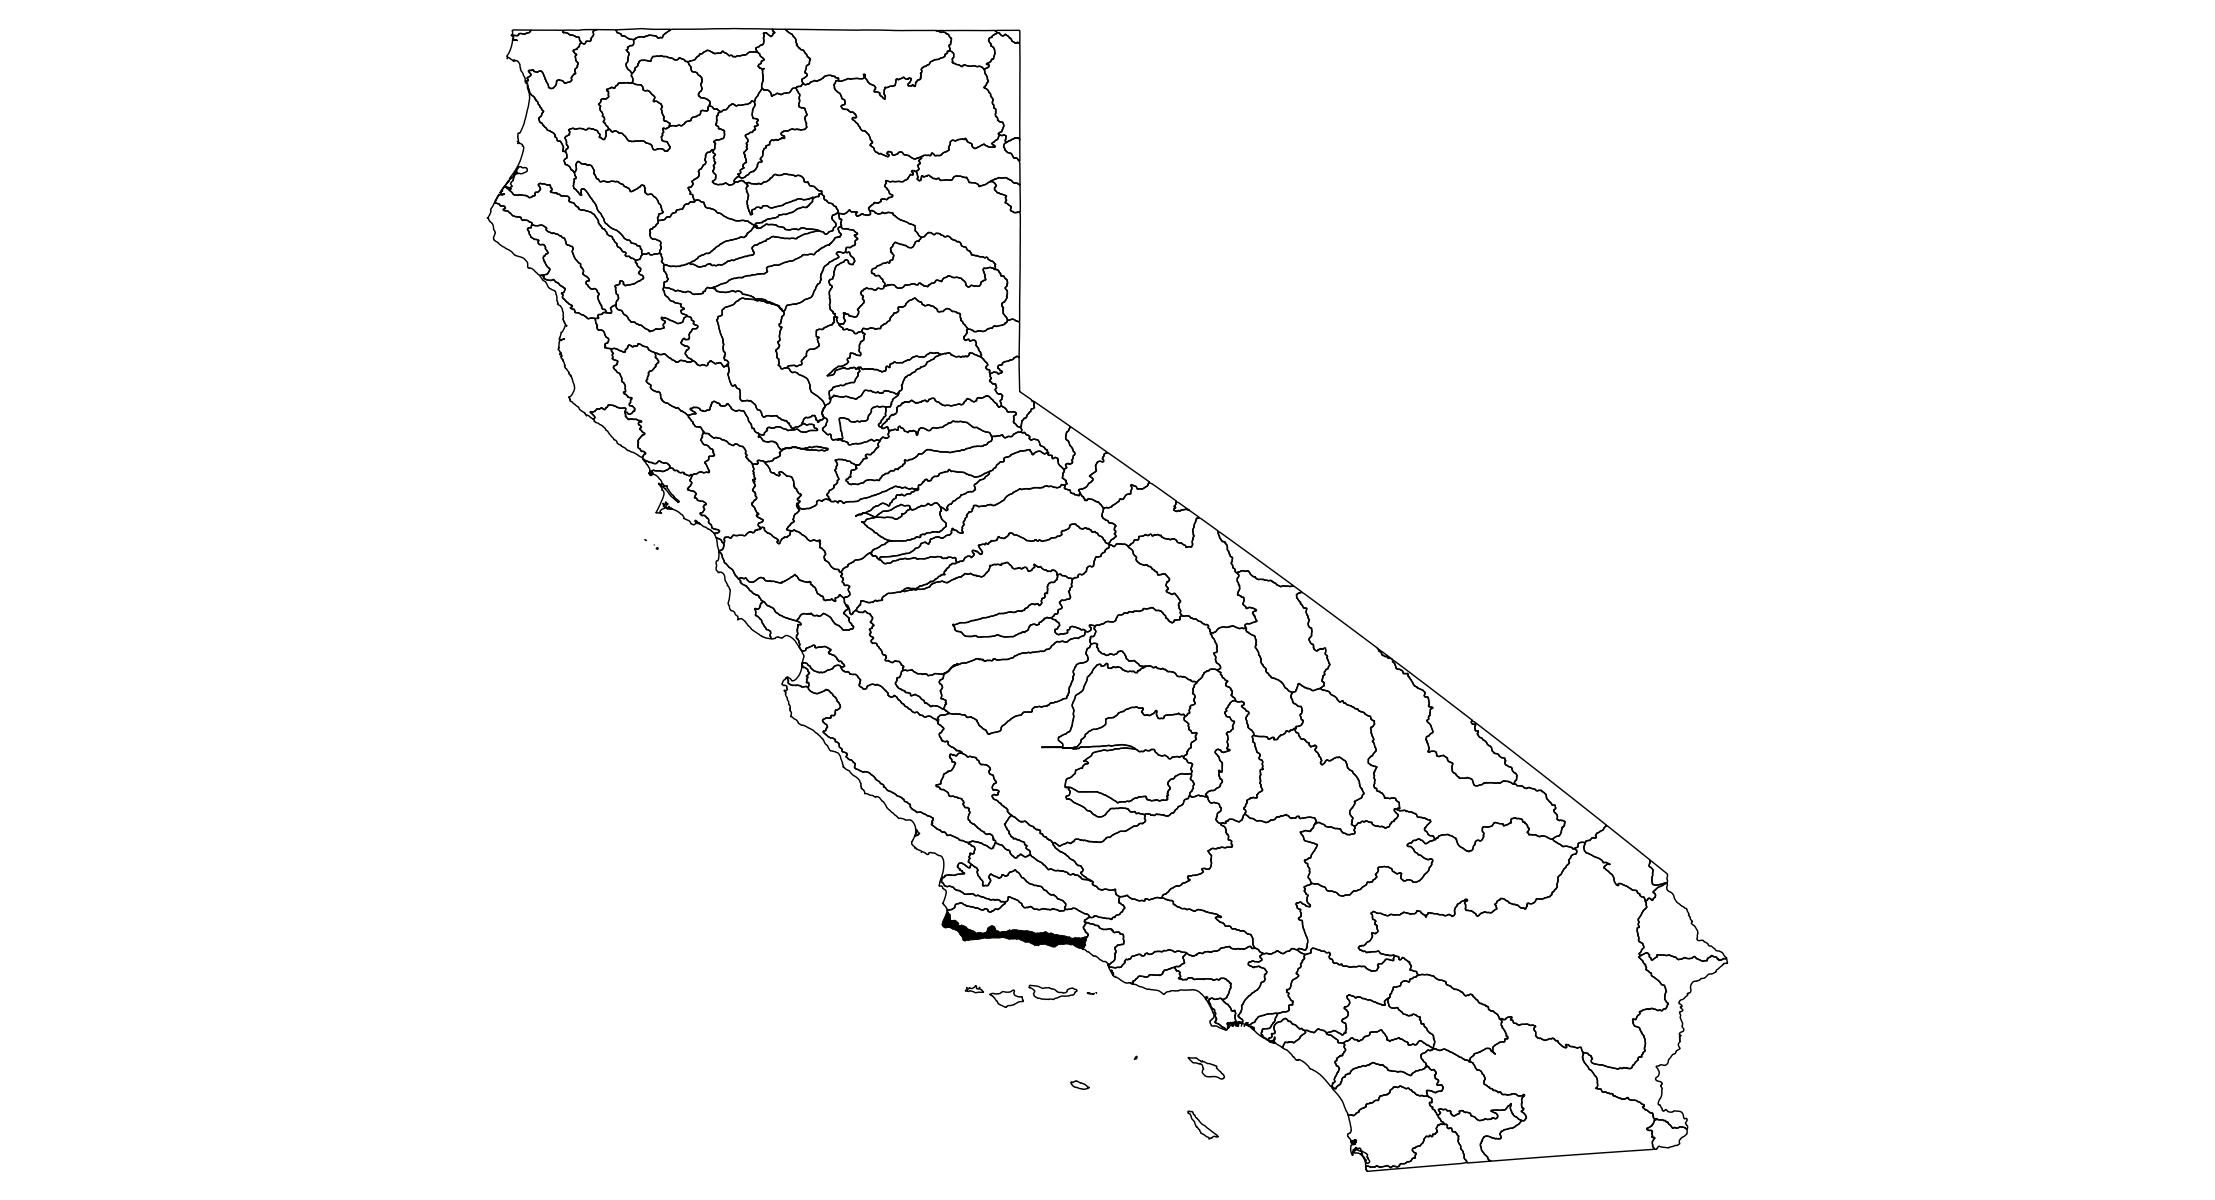
\includegraphics[width=5.5in]{figures/SantaBarbara_Overview.png}   
            \caption{Santa Barbara Region Overview (Filled in Black)}
            \label{fig:SBoverview}
            \end{center}
        \end{figure}

    \subsection{Search Domain}

The search domain used for both the weighted overlay site suitability analysis as well as the corridor location problem specification is depicted in Figure \ref{fig:SBdomain}. The extent and dimensions of this search domain is depicted in the statistics below.
    
    \begin{itemize}
      \setlength{\itemsep}{0cm}
      \setlength{\parskip}{0cm}
        \item Grid Dimensions: $363$ $cells$ x $1351$ $cells$
        \item Grid Cell Resolution: $100$ $m$ x $100$ $m$ ($1$ $ha$)
        \item Feasible Grid Cells: $117,363$ $cells$
    \end{itemize}
    
        \begin{figure}[!h]
            \begin{center}
            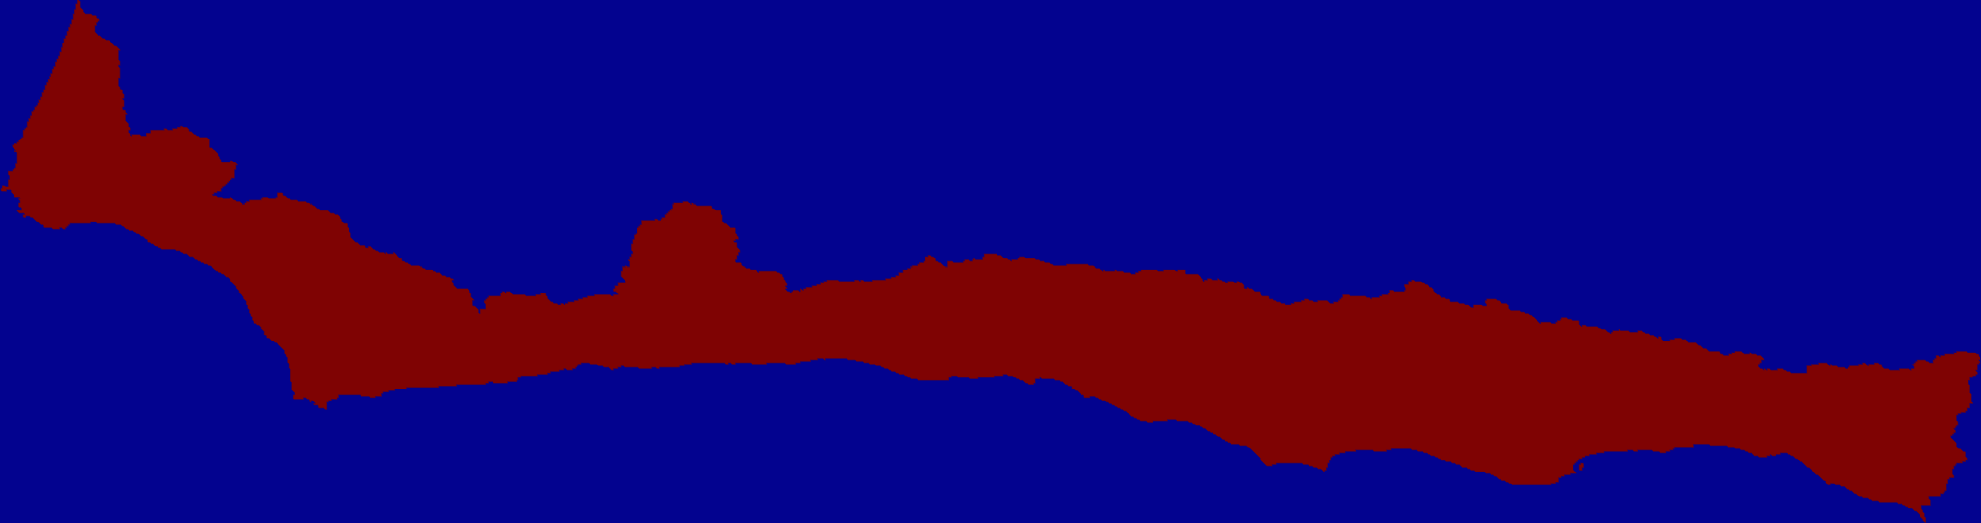
\includegraphics[width=5.5in]{figures/SantaBarbara_SearchDomain.png}   
            \caption{Santa Barbara Region Search Domain (Filled in Red)}
            \label{fig:SBdomain}
            \end{center}
        \end{figure}
        
    \subsection{Destination Search Inputs}

There are three key inputs to the weighted overlay analysis used to determine the location and extent of suitable sites for the implementation of artificial groundwater recharge basins within the region. The four layers which were generated as the discrete inputs to the WOA procedure are depicted in Figures \ref{fig:SBdsinputs_slope} through \ref{fig:SBdsinputs_landuse}. The first layer gives each cell in the search domain a score between 1 and 10 on the basis of the suitability of its slope for the implementation of a artificial groundwater recharge basin. Areas with steep slopes are given lower suitability scores. Areas with shallower slopes are given high suitability scores. 

The second input to the WOA destination search process is based upon the permeability of the surface geology as shown in Figure \ref{fig:SBdsinputs_geology}. Permeability is a crucial parameter in determining the rate of infiltration that can be achieved by a recharge basin and thus the requisite size of a basin for the purpose achieving a specified total rate of recharge. The geology score layer gives each cell in the search domain a ordinal score between 1 and 10 on the basis of the underlying surface geology layer's permeability constant.

The final input to the WOA destination search process is based upon the existing landuse as shown in Figure \ref{fig:SBdsinputs_landuse}. The existing landuse can be a proxy measure of both the cost of procurement for the landholdings required to implement the artificial recharge basin as well as the regulatory and engineering difficulty associated with artificial recharge basin implementation. Here again, these scores are have been pegged to a 1 to 10 ordinal scale that aligns with those assigned to each of the other two score layers. 

        \begin{figure}[!h]
            \begin{center}
            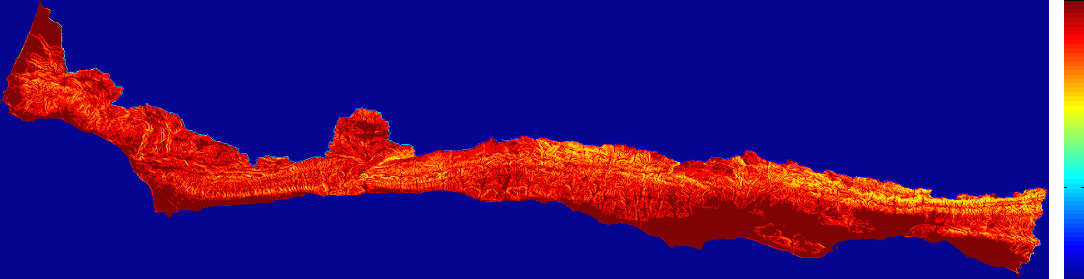
\includegraphics[width=5.5in]{figures/SantaBarbara_Search_Slope.png}   
            \caption{Santa Barbara Region Destination Search Inputs: Slope Score (Blue:Low, Red:High)}
            \label{fig:SBdsinputs_slope}
            \end{center}
        \end{figure}
        
        \begin{figure}[!h]
            \begin{center}
            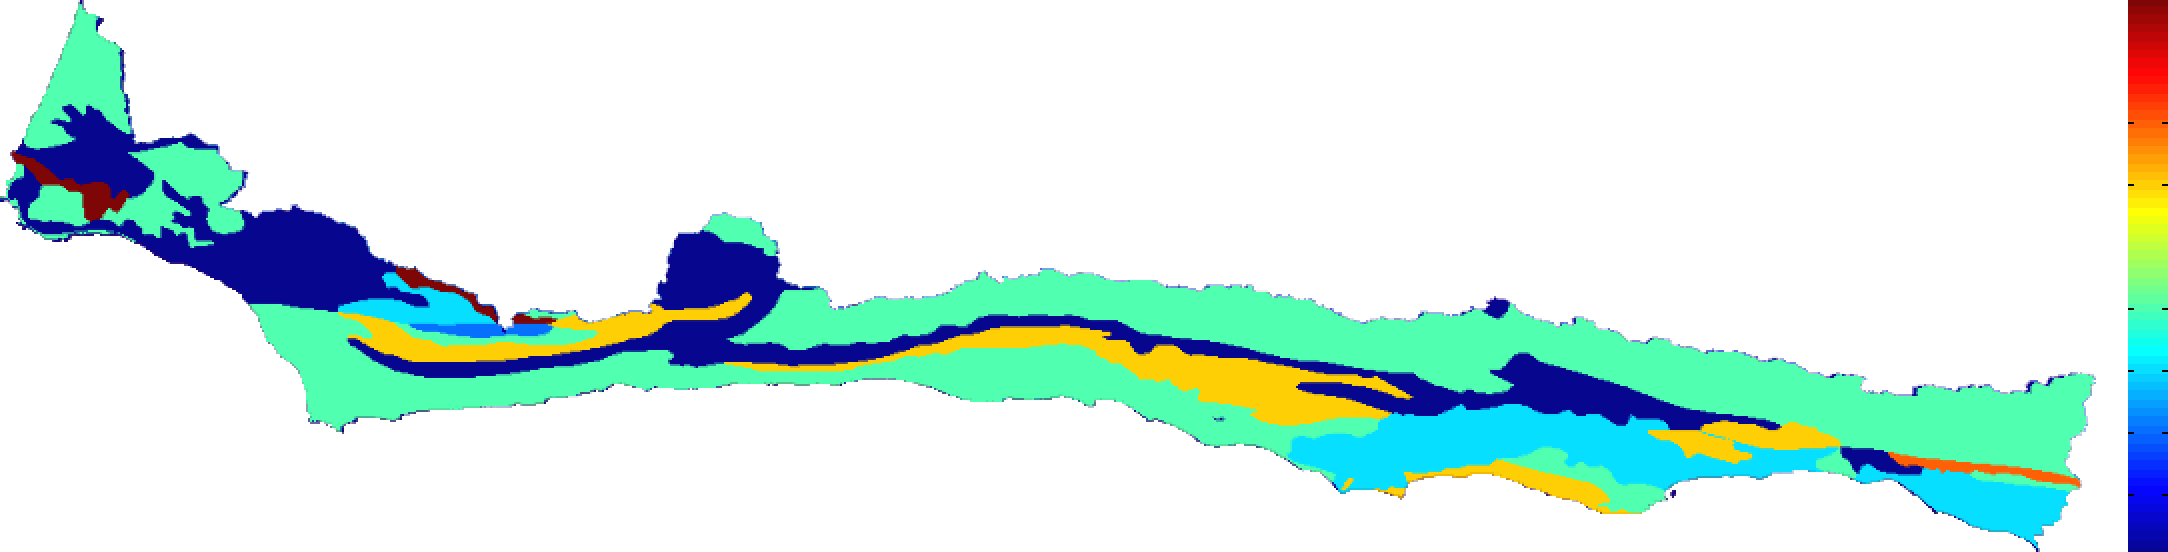
\includegraphics[width=5.5in]{figures/SantaBarbara_Search_Geology.png}   
            \caption{Santa Barbara Region Destination Search Inputs: Geology Score (Blue:Low, Red:High)}
            \label{fig:SBdsinputs_geology}
            \end{center}
        \end{figure}
    
        \begin{figure}[!h]
            \begin{center}
            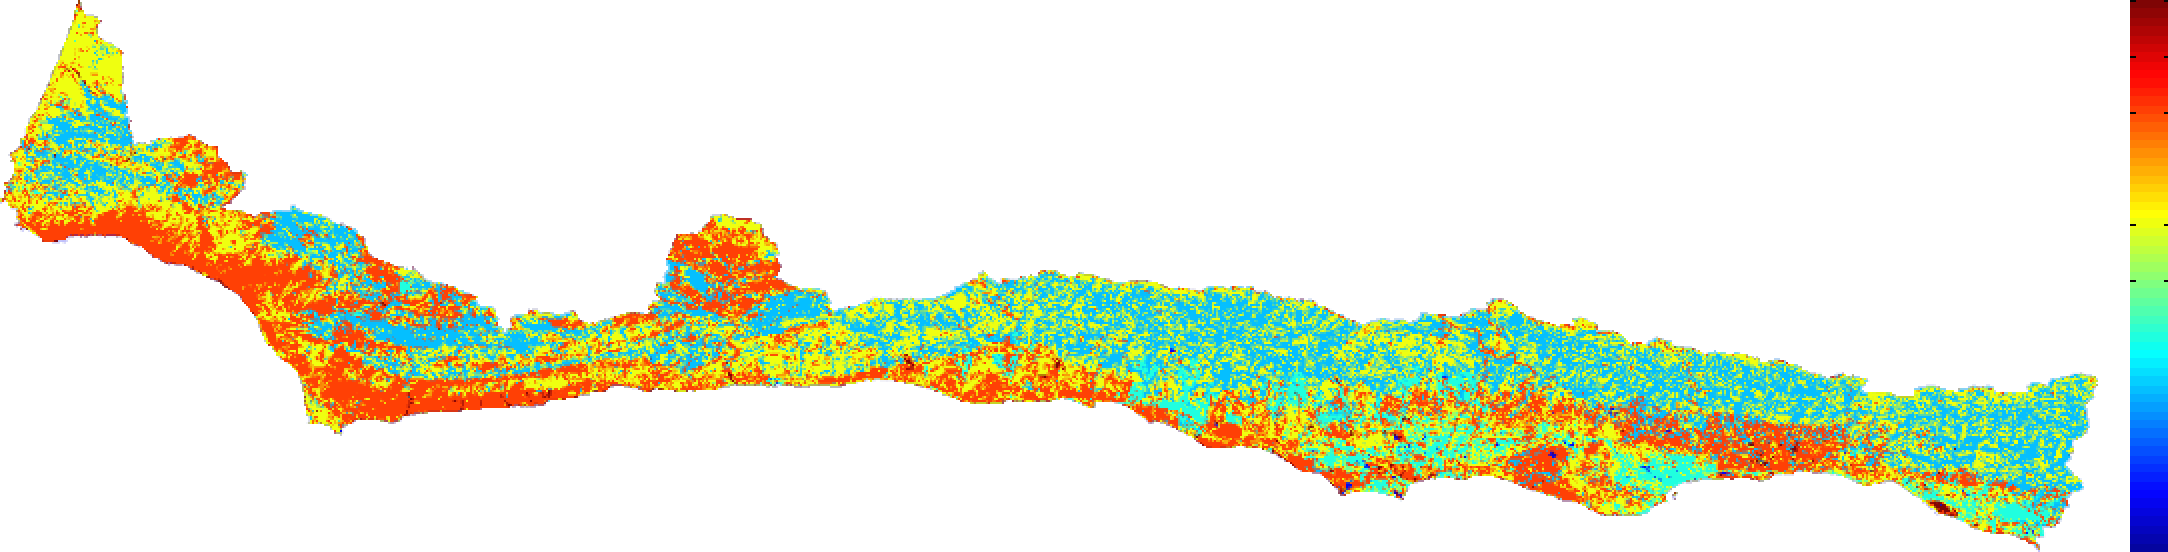
\includegraphics[width=5.5in]{figures/SantaBarbara_Search_Landuse.png}   
            \caption{Santa Barbara Region Destination Search Inputs: Landuse Score (Blue:Low, Red:High)}
            \label{fig:SBdsinputs_landuse}
            \end{center}
        \end{figure}
    
    \subsection{Destination Search Outputs}
    
The raw output of the WOA destination search process is a composite layer of which depicts a measure of overall suitability for the given landuse application on an ordinal scale as in Figure \ref{fig:SBdsoutputs_comp}. This single composite suitability layer is then thresholded, selecting only those areas that have the highest composite suitability scores as shown in Figure \ref{fig:SBdsoutputs_cand}. A set of morphological operations is applied to this threshold mask which ranks each connected area of high suitability in terms of its size. Larger connected areas of high suitability are considered better in this process and thus, in this way, a single destination location for the corridor search process can be automatically selected as the single largest area of high aggregate suitability with the study area. 
    
        \begin{figure}[!h]
            \begin{center}
            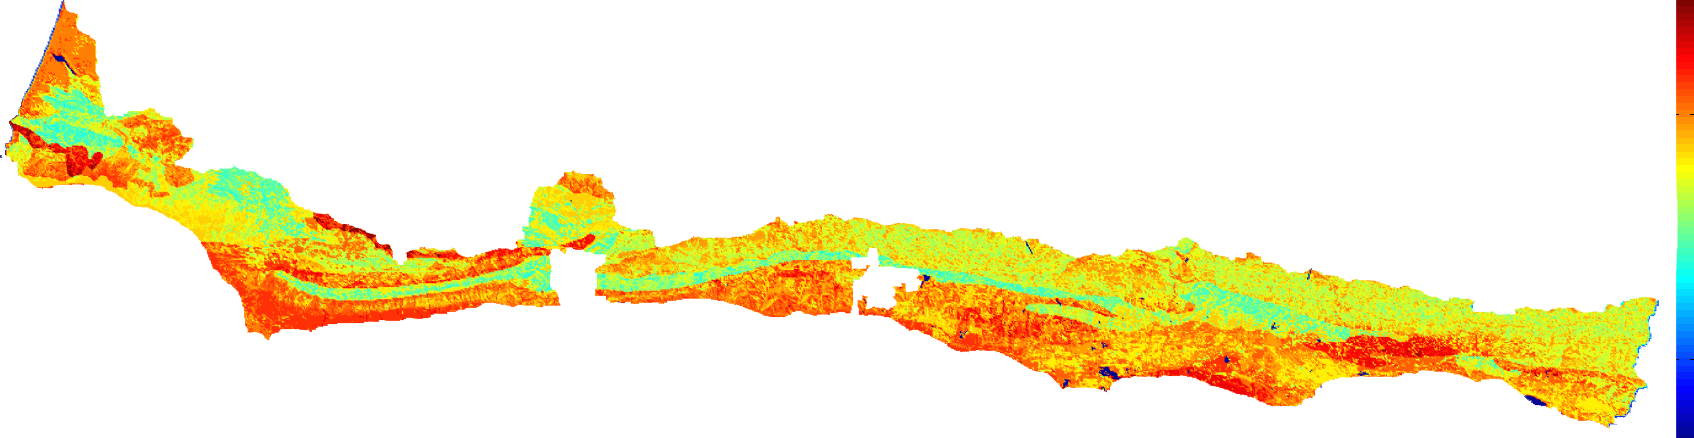
\includegraphics[width=5.5in]{figures/SantaBarbara_Search_Composite.png}   
            \caption{Santa Barbara Region Destination Search Outputs: Composite Scores (Blue:Low, Red:High)}
            \label{fig:SBdsoutputs_comp}
            \end{center}
        \end{figure}
        
        \begin{figure}[!h]
            \begin{center}
            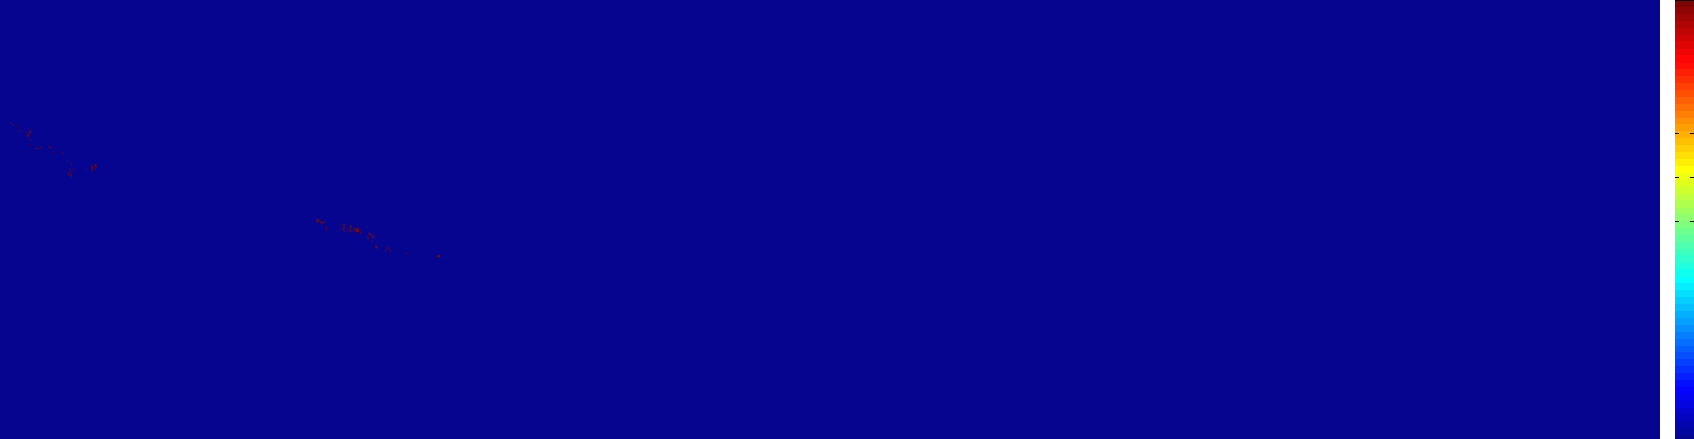
\includegraphics[width=5.5in]{figures/SantaBarbara_Search_Output.png}   
            \caption{Santa Barbara Region Destination Search Outputs: Candidate Regions}
            \label{fig:SBdsoutputs_cand}
            \end{center}
        \end{figure}

    \subsection{Proposed Corridor Endpoints}
    
For the Santa Barbara case study region, the final output of the WOA analysis is shown in Figure \ref{fig:SBendpoints} in red and mapped relative to the location of the source location for the corridor location analysis that corresponds to the location of the largest WWTP within the basin, in green. These two points, plus the extent of the search domain, form the basis of the corridor location problem specification that is to be discussed in further detail in the subsequent section. 
    
    \begin{itemize}
      \setlength{\itemsep}{0cm}
      \setlength{\parskip}{0cm}
        \item Start Location: $(313,1083)$
        \item End Destination: $(248,886)$   
        \item Shortest Euclidean Path Distance: $20,745$ $m$ ($21$ $km$) 
    \end{itemize}
    
        \begin{figure}[!h]
            \begin{center}
            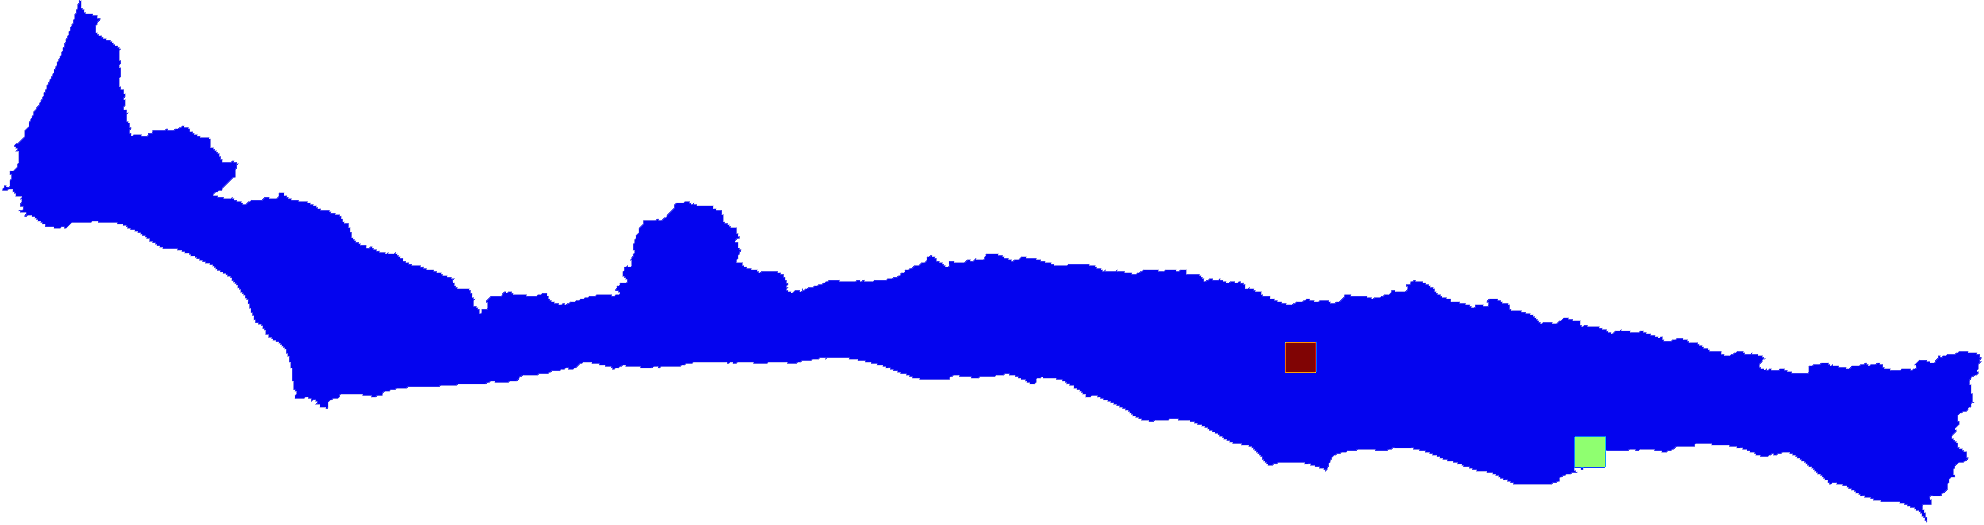
\includegraphics[width=5.5in]{figures/SantaBarbara_Endpoints.png}   
            \caption{Santa Barbara Region Proposed Corridor Endpoints}
            \label{fig:SBendpoints}
            \end{center}
        \end{figure}
            
    \subsection{Proposed Objective Layers}
    
For the corridor location problem specification used as the input to the MOGADOR algorithm, four key pieces of information are required. The first three correspond to the source location, the destination location, and the search domain boundaries that have been previously described. The forth key input category corresponds to the objective score layers which capture the cost associated with routing sections of a corridor over each grid cell in the search domain. For this analysis, the following three distinct objectives were developed.

The first objective category is based upon the accessibility of each location for the purposes of constructing and maintaining the water distribution infrastructure that the corridor is designed to support and is shown in Figure \ref{fig:SBaccessibility}. It is fundamentally easier to get materials and people to a locations that are positioned along road networks. As a result, the underlying road network topology was used to encode a continuous objective score layer with values ranging from 1 to 10 that can be described as a measure of "Accessibility" and which favors those locations that are on and around roads.

The second objective category is based upon the existing land use regime within the regional search domain. The idea behind the composition of this objective can be thought of as somewhat of the converse of Accessibility in the sense that, regions which are already heavily developed are likely to be socially, politically, or economically challenging to implement corridors for large scale water distribution pipeline infrastructure. Using standardized USGS based land use classification, each grid cell in the search domain is given a nominal objective score value from 1 to 10  corresponding the relative level of "Disturbance" that would be associated with routing a corridor across it. This objective layer is depicted in the layer plotted in Figure \ref{fig:SBdisturbance}.

The third objective category is derived from the underlying slope within the search domain. Steeper slopes are assigned a higher ordinal score, ranging from 1 to 10. This objective reflects the desire for corridors to be shorter in length and minimally accumulate slopes over their length. In this way, the slope score provides a mechanism for the corridor routing algorithm to preferentially favor corridors that would have minimal energy requirements in terms of the operational energy requirements of the anticipated water distribution infrastructure. This slope score objective layer is depicted in Figure \ref{fig:SBslope}. 

        \begin{figure}[!h]
            \begin{center}
            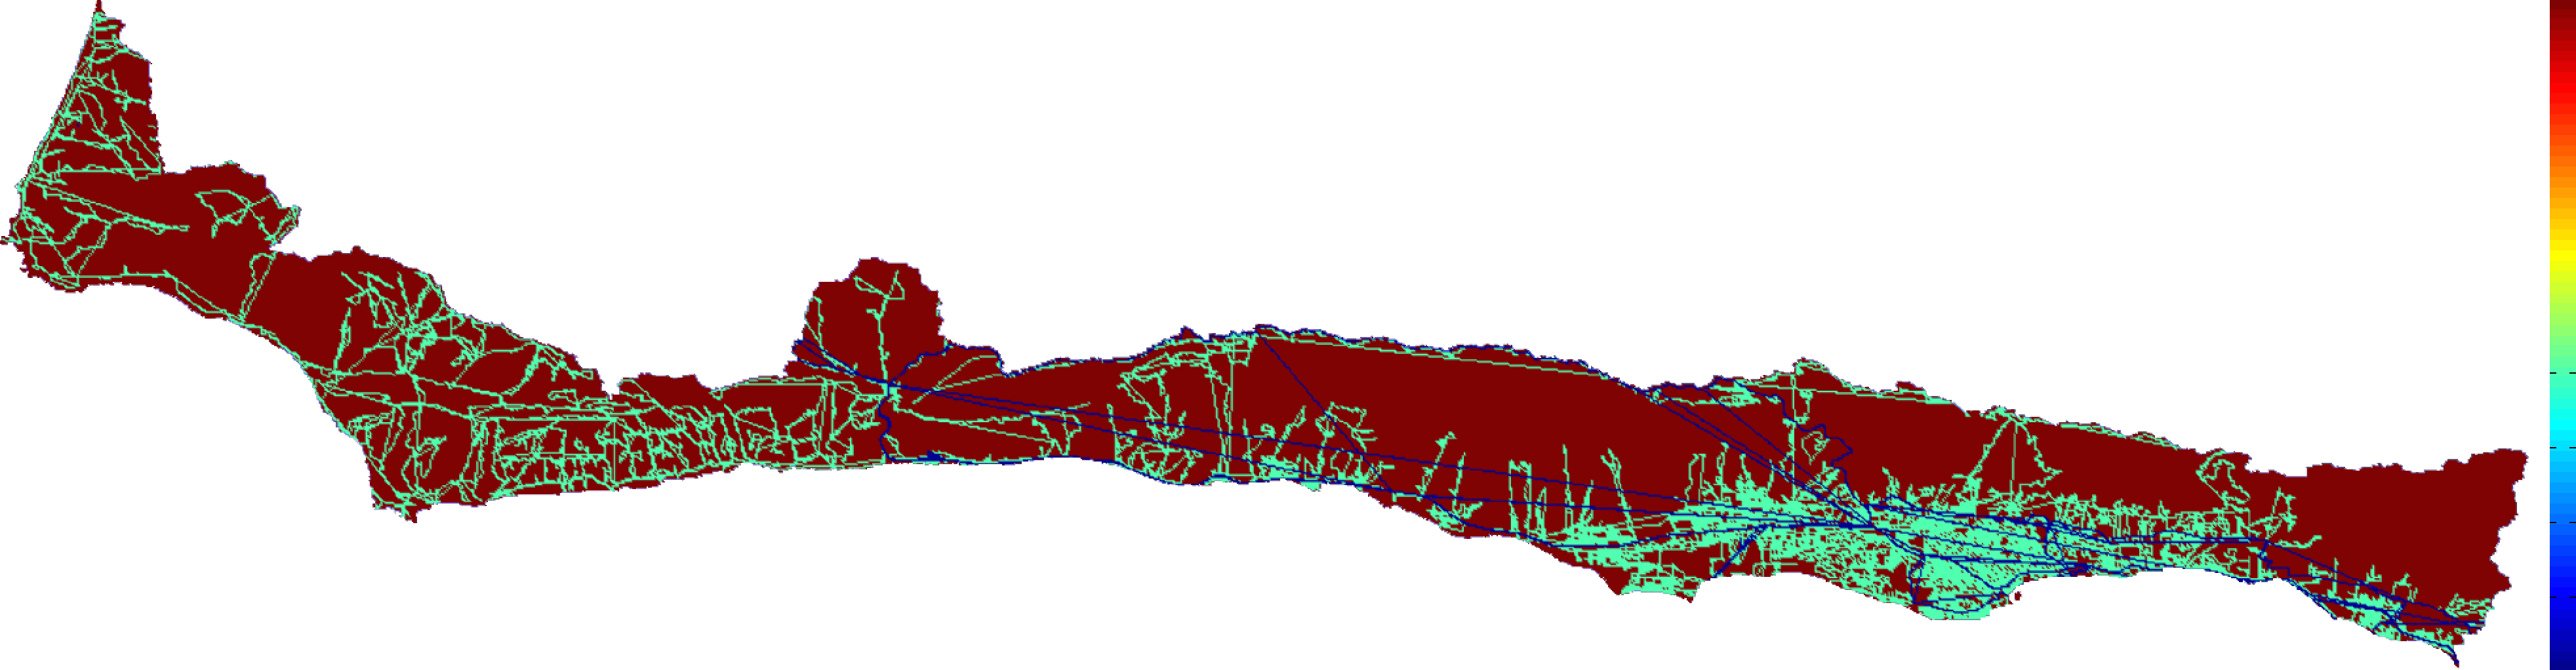
\includegraphics[width=5.5in]{figures/SantaBarbara_AccessibilityScore.png}   
            \caption{Santa Barbara Region Accessibility Based Objective Scores (Blue:Low, Red:High)}
            \label{fig:SBaccessibility}
            \end{center}
        \end{figure} 

        \begin{figure}[!h]
            \begin{center}
            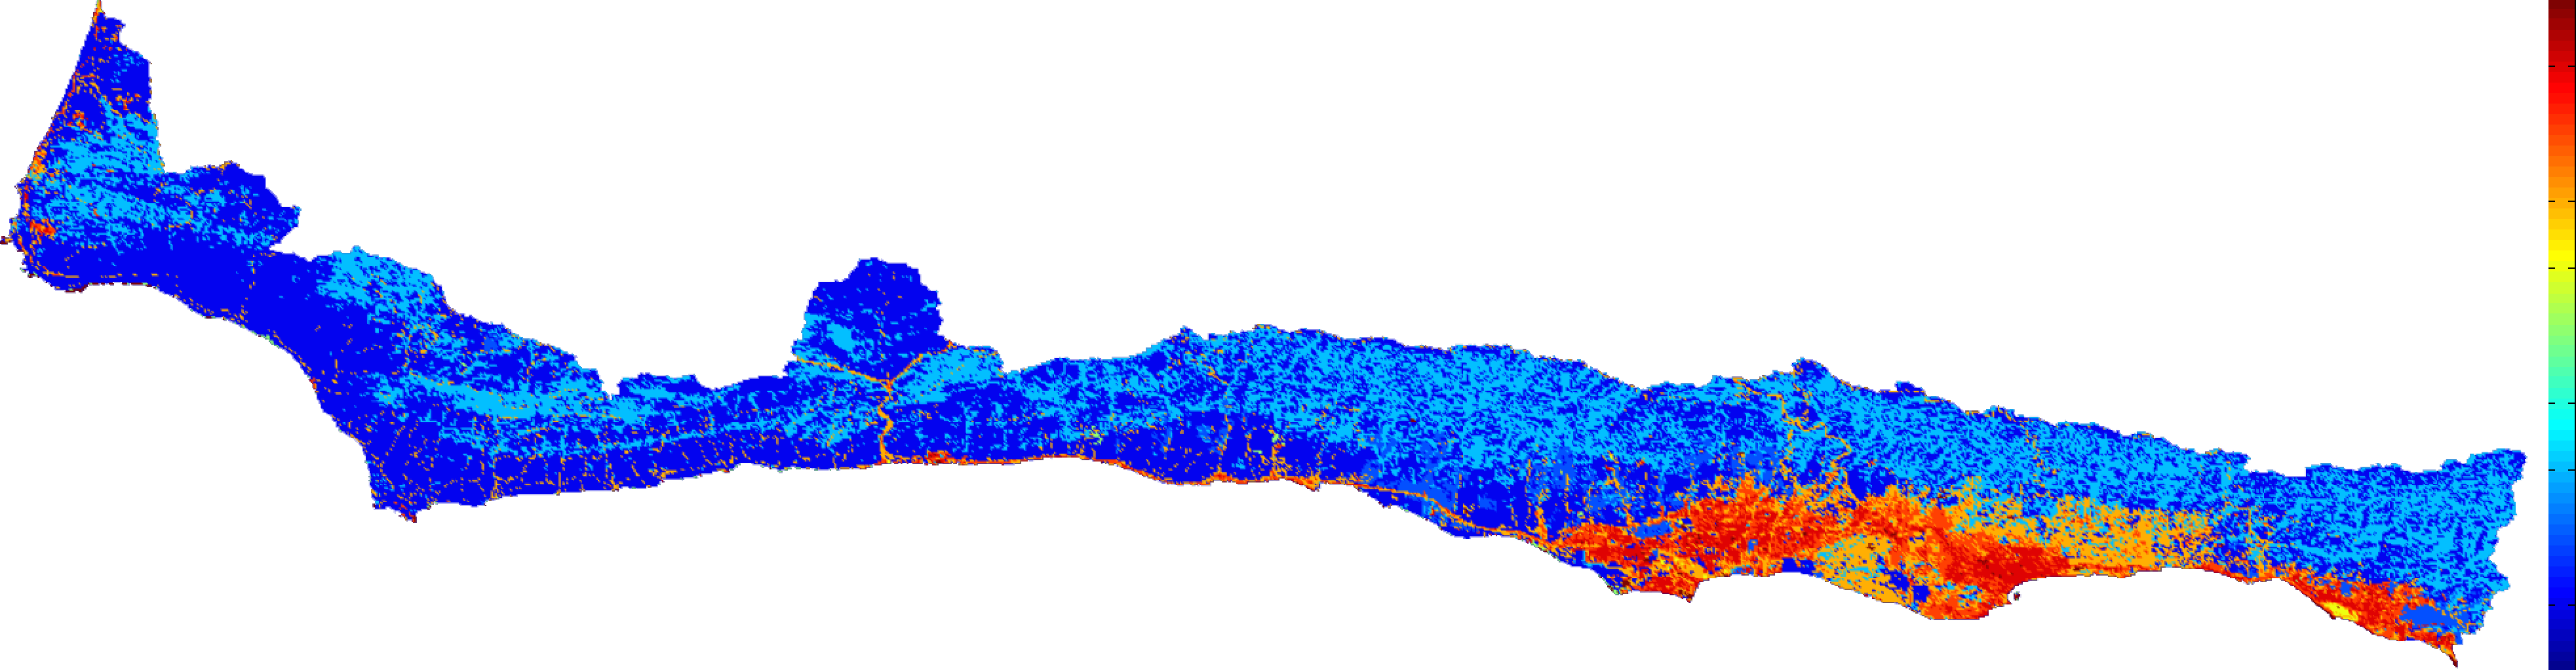
\includegraphics[width=5.5in]{figures/SantaBarbara_DisturbanceScore.png}   
            \caption{Santa Barbara Region Land Use Disturbance Based Objective Scores (Blue:Low, Red:High)}
            \label{fig:SBdisturbance}
            \end{center}
        \end{figure}
        
        \begin{figure}[!h]
            \begin{center}
            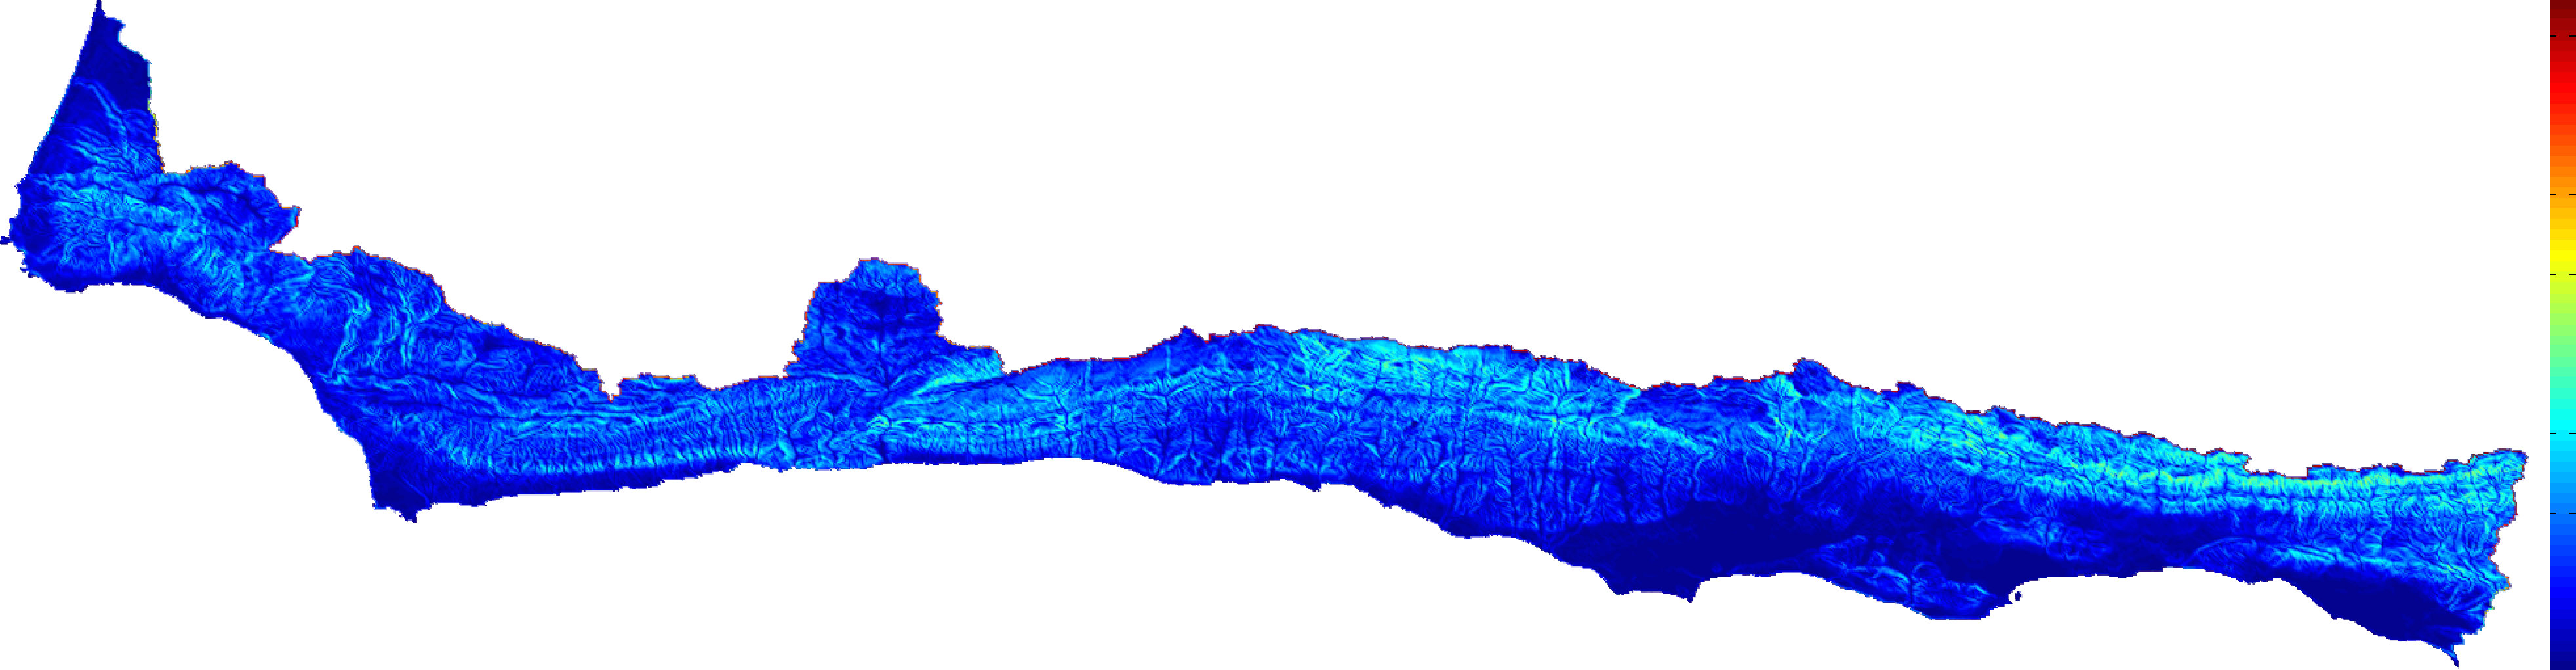
\includegraphics[width=5.5in]{figures/SantaBarbara_SlopeScore.png}   
            \caption{Santa Barbara Region Slope Based Objective Scores (Blue:Low, Red:High)}
            \label{fig:SBslope}
            \end{center}
        \end{figure}
        
    \subsection{Proposed Corridor Solutions}
    
Shown in Figure \ref{fig:SBresults} are the outputs of a series of three runs of the MOGADOR algorithm for the Santa Barbara region problem specification. These three runs differ solely in terms of the number of individuals contained within the seed population. The size of this seed population determines the extent with which the input search domain is search and, consequently, the degree to which the output solution corridor is likely to approximate the global optimal solution. The figure contains six panes made up of three rows and three columns. The columns depict, from left to right, and plan view of the final output solution set, and line plot of the break down of objective scores for the top 100 ranked individuals in the final output solution set, and, finally, a histogram plot of the frequency of total aggregate objective scores among the same top 100 individuals. Alternatively, the rows, moving from top to bottom, reflect the changing results as the population size is increased from 1,000 to 10,000 to 100,000. 

As the histogram plots of the aggregate objective scores illustrate, with a population size of 100,000 the aggregate objective scores are quite low, and the quality of the final output solution set is very high. This improvement in solution quality comes at the expense of processing time/effort. This tradeoff shall be discussed in greater detail and illustrated comparatively across all of the five case studies at the end of this chapter. 

One interesting feature of this exercise which can be readily appreciated from this set of plots is the source of the improvement in the aggregate objective scores between the different runs. For example, note the height of the data series depicted by the blue line, corresponding to the accessibility score, in the three plots in the middle column. The progressive decrease in the values associated with this line indicates that the reduction in aggregate objective scores between the three runs can be attributed to a reduction in the Accessibility score. This is tantamount to saying that the search process is able to provide better solutions as it "Finds the road network." And indeed, this conclusion is reflected from a simple visual inspection of the output corridors plotted in the panels contained in the first column. Here it can be seen that in the 100,000 population size solution set, the pathway sections have become much more linear, and appear to correspond with the layout of different road segments which occupy the area in between the source and the destination. 
    
        \begin{figure}[!h]
            \begin{center}
            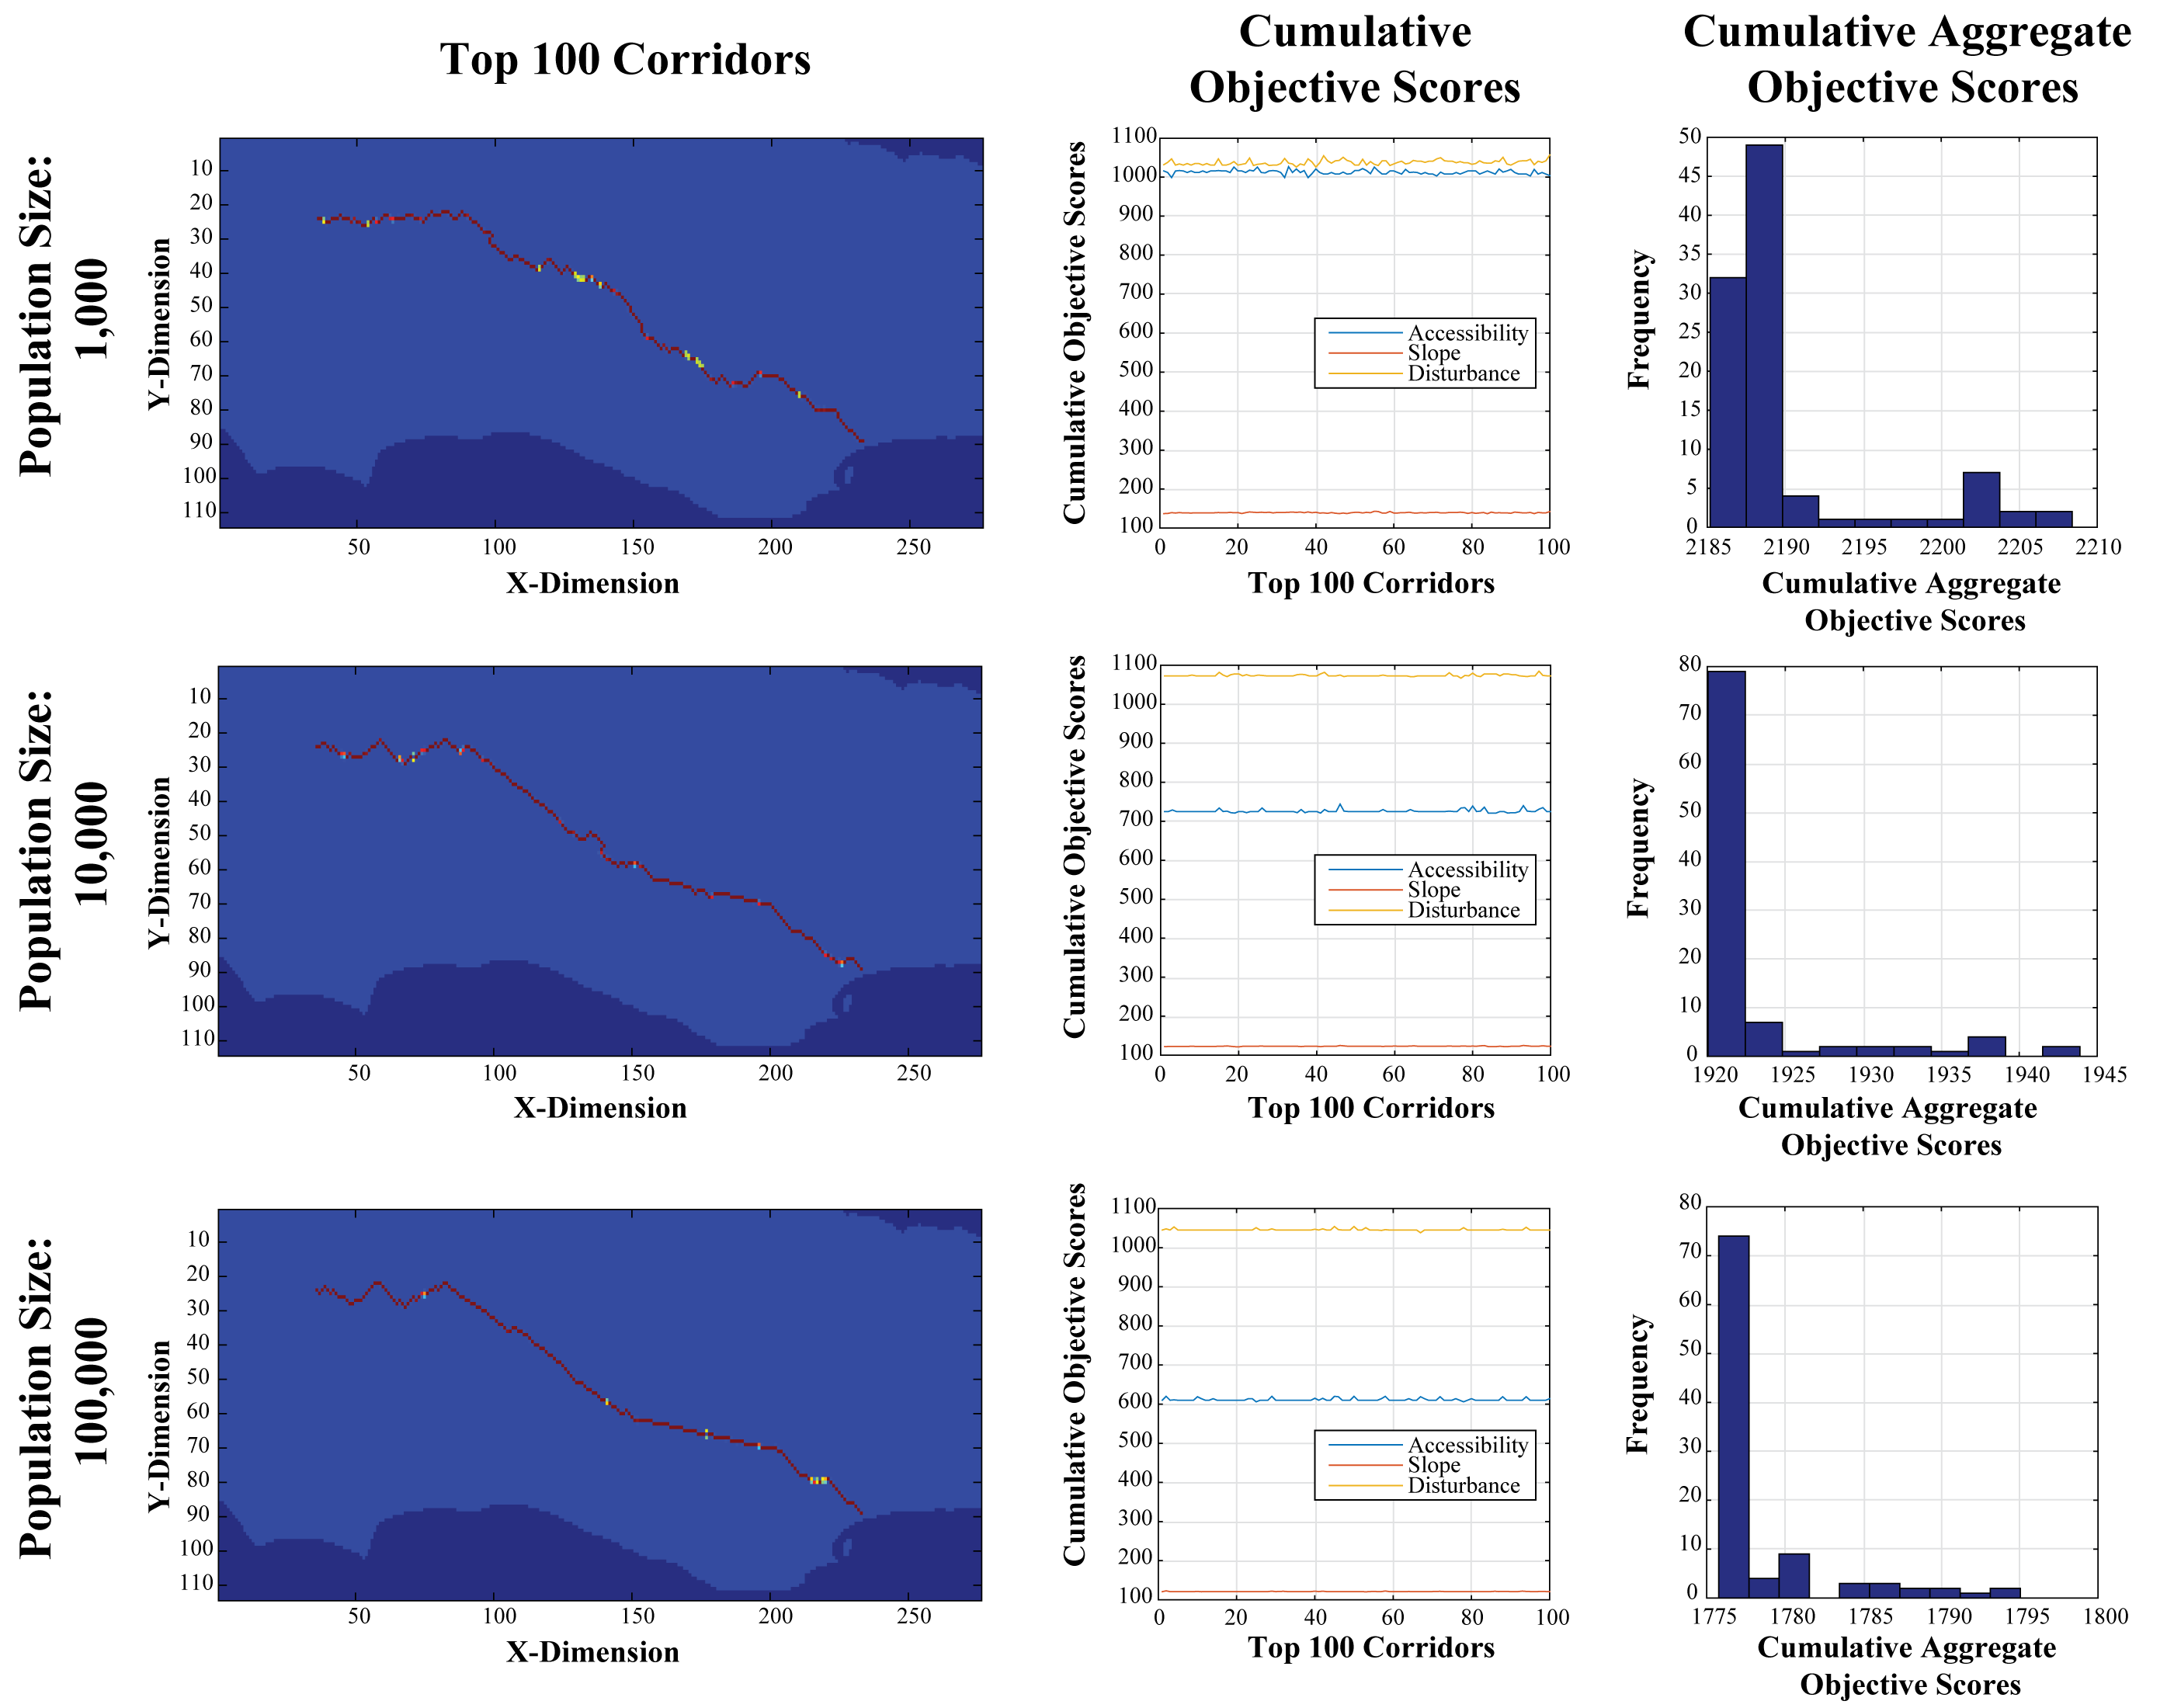
\includegraphics[width=6in]{figures/SantaBarbara_PathwayResults.png}   
            \caption{Santa Barbara Region Corridor Analysis Results}
            \label{fig:SBresults}
            \end{center}
        \end{figure}
        
Figure \ref{fig:SBelevationProfile} provides an illustration of the top ranked final output corridor solution presented in the context of the full search domain. For all of the case studies the highest quality solution was developed by the model run containing the largest seed population. This was fully expected however and is in good agreement with the theoretical discussion of the role of the population initialization procedure in the behavior of the MOGADOR algorithm described in Chapter 3. l

        \begin{figure}[!h]
            \begin{center}
            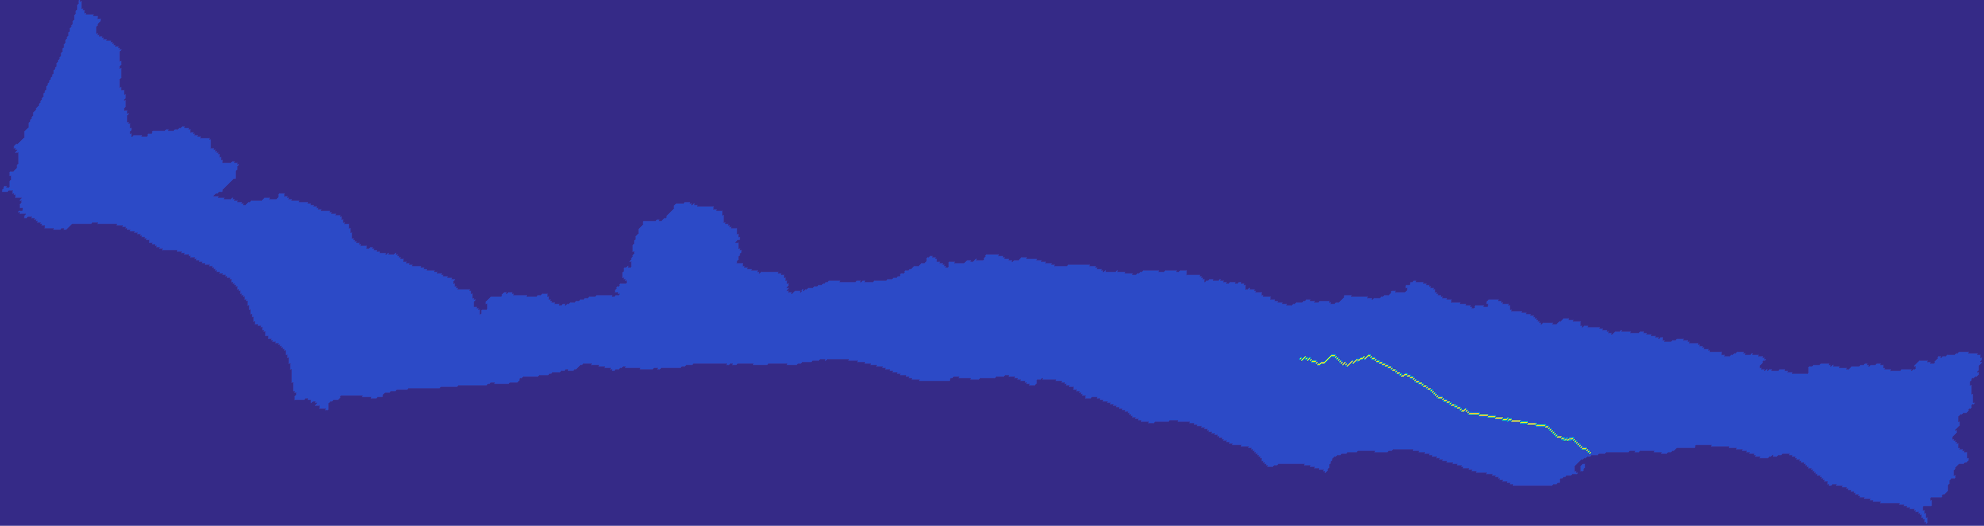
\includegraphics[width=5.5in]{figures/SantaBarbara_PathwayLarge.png}   
            \caption{Santa Barbara Region Top 100 Corridors (Pop Size: 100,000) Basin Wide Overview}
            \label{fig:SBsolutionOverview}
            \end{center}
        \end{figure}
        
    \subsection{Along-Corridor Elevation Profile}
    
Figure \ref{fig:SBelevationProfile} illustrates the along-corridor elevation profile that can be generated by superimposing the output corridor solution on top of a regional digital elevation model for the Santa Barbara region. As the Figure shows the total elevation gain between the source and the destination location is a modest 200 meters across a distance spread of roughly 25 kilometers. While it may appear that the corridor has a significant amount of vertical fluctuations, these are minor in absolute terms, and stem from the fact that the slope score -- the objective most directly related to the corridor elevation profile structure -- was but only one of three in the multi-objective problem statement. These elevation fluctuations therefore can be thought of as the result of a profitable tradeoff between the accumulation of smoother slopes and more favorable values for the other two objectives. 
        
        \begin{figure}[!h]
            \begin{center}
            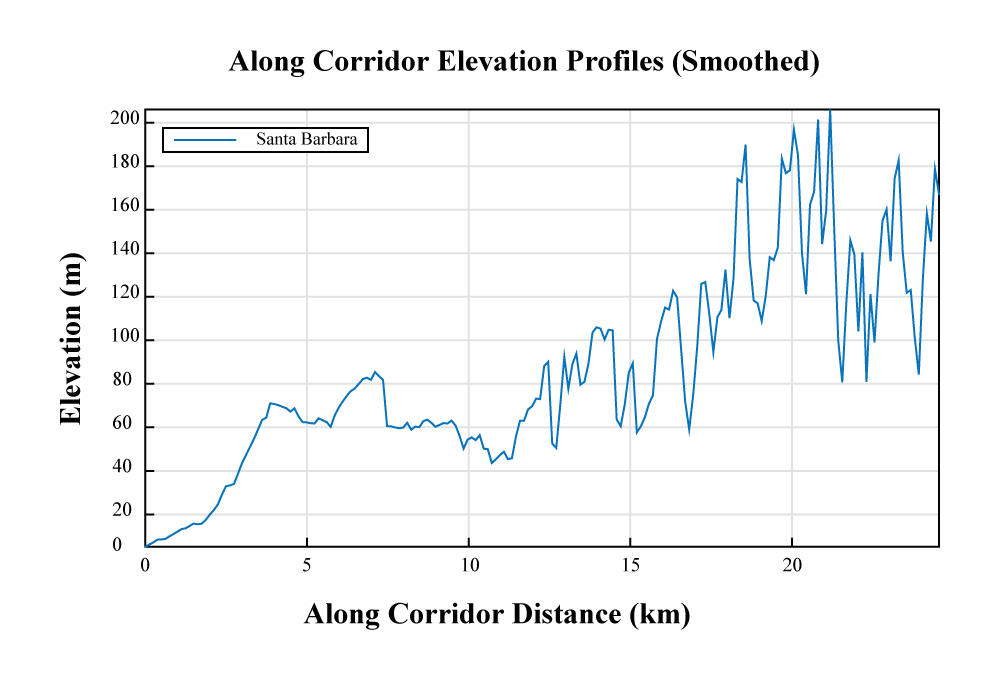
\includegraphics[width=5.5in]{figures/SantaBarbara_Elevation_Profile.png}   
            \caption{Santa Barbara Region Proposed Corridor Elevation Profile}
            \label{fig:SBelevationProfile}
            \end{center}
        \end{figure}
        
\clearpage
    
\section{Oxnard Region}

The second case study region consists of the HUC-8 zone containing the Oxnard plain and its immediate surrounding territories stretching as far inland as Ojai. This second case study region is located nearly adjacent to the first -- separated only by a single HUC-8 basin. The reason for the choice of two case study regions in such close physical proximity is down to the recent implementation of a functioning large scale water reuse system by the municipal water management district there. 

The majority of this HUC-8 zone's area is a comprised of a broad low lying alluvial plain. This plain has found rich application within the agricultural sector, supporting the production of a wide variety of row crops as well as high value orchard stands. Over the past three decades, the region has also experience significant population growth with sprawling suburban communities encroaching into the more marginal farmlands or those held by smaller independent farmers. The combined freshwater demands of these two sectors have conspired to create a persistent imbalance between freshwater supply and demand in this coastal region. 

Oxnard's struggle with freshwater management issues can be traced as far back as 1937 when the USGS identified that sustained groundwater pumping to support the irrigation of surface crops was contributing to the depletion of the underlying aquifer and inviting the intrusion of brackish seawater into the subsurface hydrologic strata. In response to this issue, the local municipal water authority enacted a program in which a portion of the regions' agricultural water was diverted towards a series of subsurface injection wells -- strategically positioned along the coast -- through which freshwater would be pumped to created an artificial pressure head barrier to prevent further intrusion of seawater, and thus further contamination of the aquifer. 

This program has operated successfully for a number of decades now; achieving a functional equilibrium between the level of groundwater pumping occurring within the basin and the amount of water the is delivered to the artificial intrusion barrier. More recently however, decreases in available freshwater supply due to a persistent statewide drought have forced municipal water managers in this region to thing more proactively about developing alternative sources of water supply. This process began with the creation of a plant to substitute potable freshwater for reclaimed brackish water for use in the subsurface barrier injection wells. 

The successful operation of this plant for a number of years inspired enough confidence among the water resource management authorities in this area to pursue and very recently achieve a goal of implementing a facility capable of reclaiming and reusing the growing volume of municipal wastewater being generated within the basin. This new facility, commissioned just this year, provides the capability to treat 100\% of the wastewater generated in the basin to a potable standard through a complex treatment chain incorporating a sophisticated chain of tertiary treatment processes including: advanced micro-filtration, reverse osmosis, ultraviolet filtration, and ozonation. The long term plan for the water currently being produced by this facility is for groundwater recharge at higher elevation locations within the basin. As such, this locale represents the ideal candidate for evaluation in this study. 

    \subsection{Regional Context}
    
    \begin{itemize}
      \setlength{\itemsep}{0cm}
      \setlength{\parskip}{0cm}
        \item HUC-8 Code: $18070102$
        \item Total Area: $5,188.3$ $km^2$
        \item Maximum Elevation: $2,664.4$ $m$
        \item Minimum Elevation: $-0.05$ $m$
        \item Mean Slope: $15.54$ $\%$
        \item Standard Deviation of Slope: $11.11$ $\%$
        \item Dominant Soil Composition: Hydrologic Soil Group - B: $10-20\%$ clay, $50-90\%$ sand, $35\%$ rock fragments
    \end{itemize}
    
        \begin{figure}[!h]
            \begin{center}
            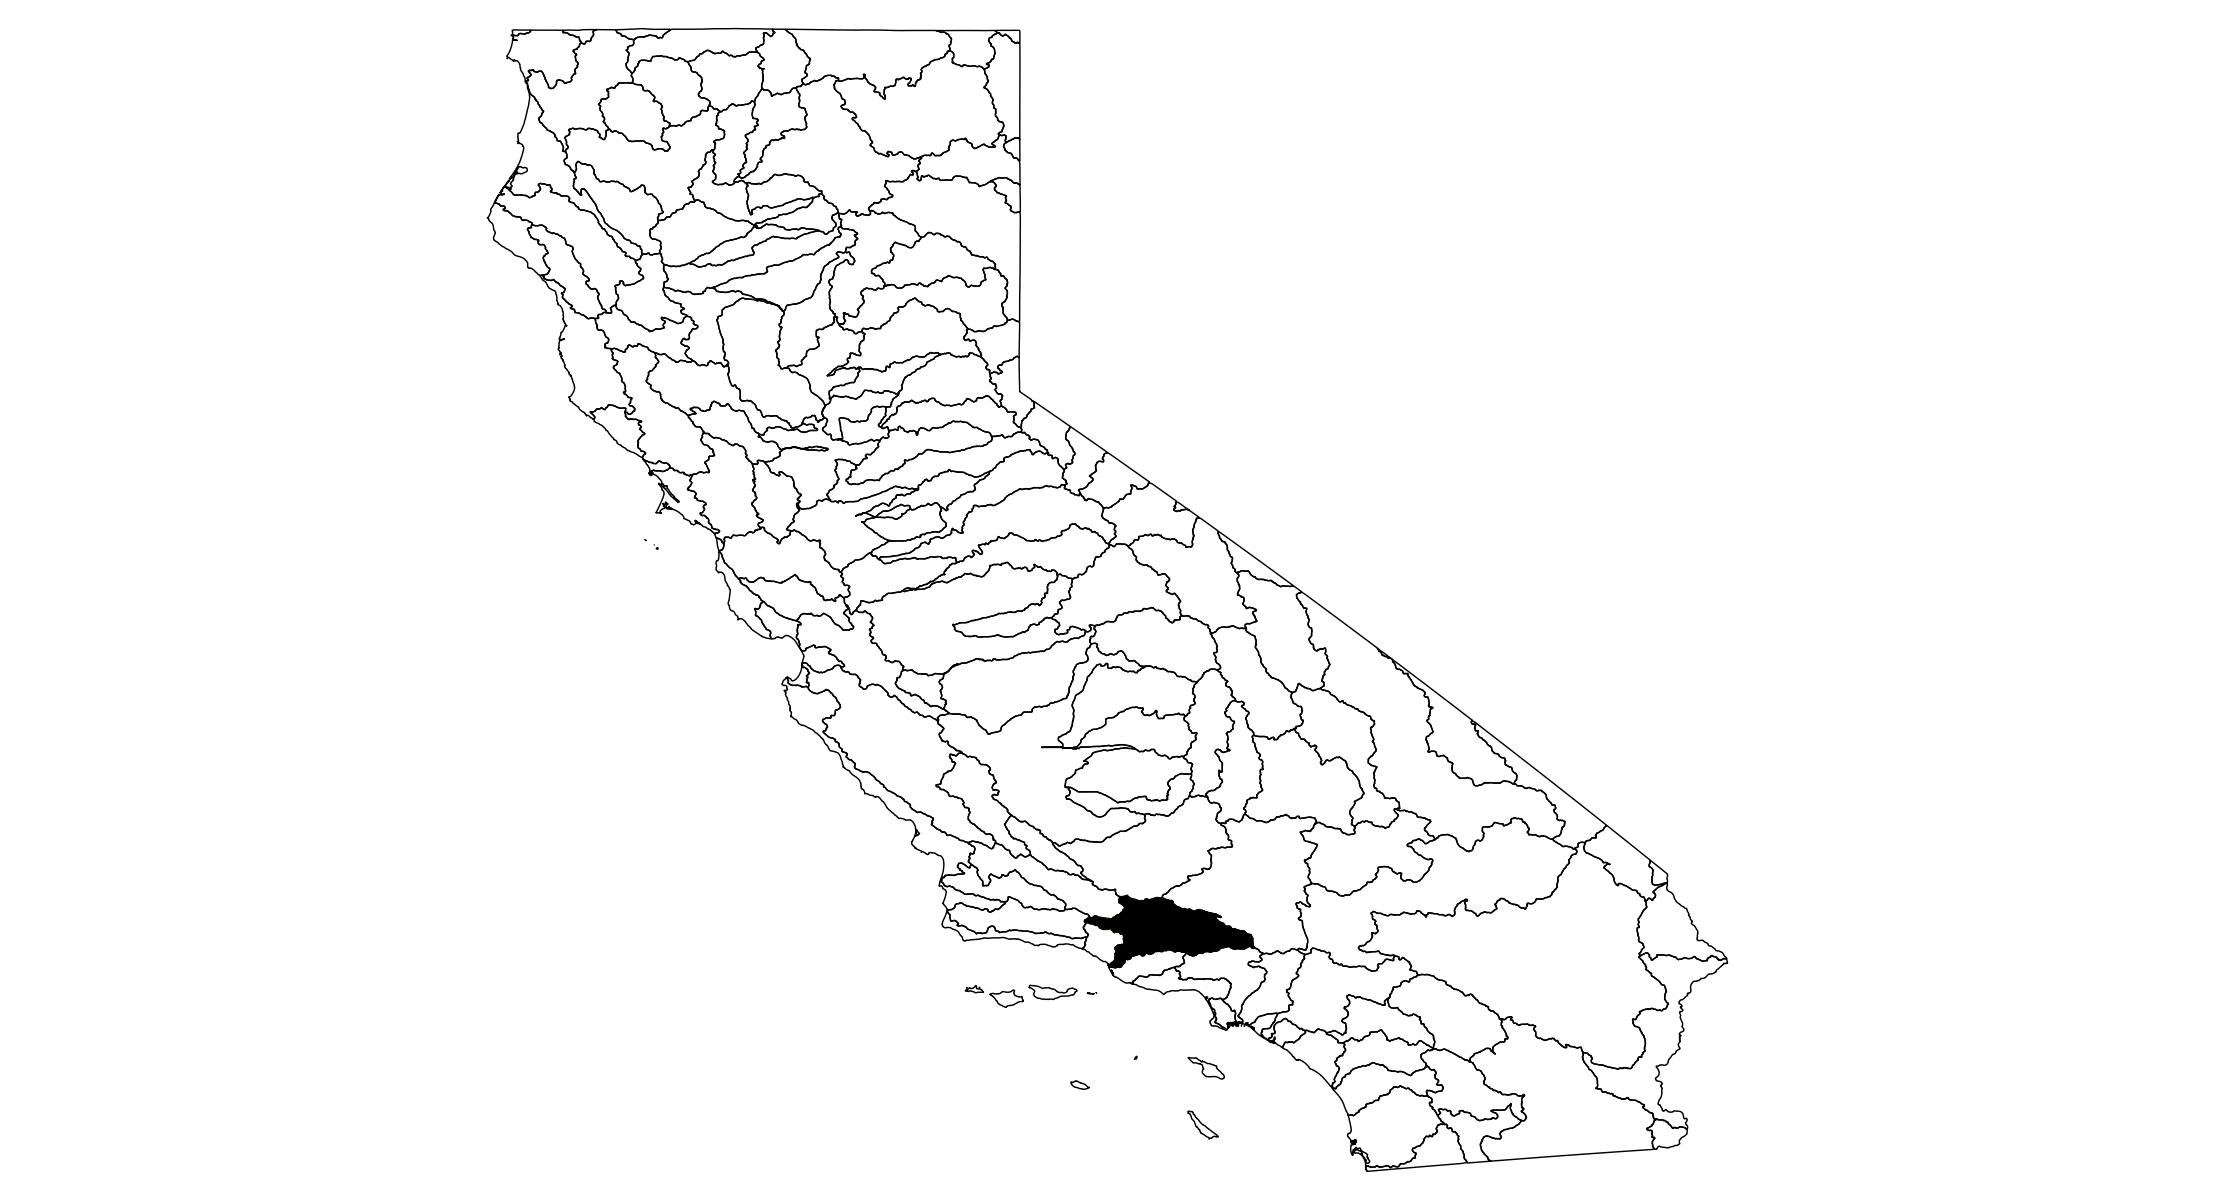
\includegraphics[width=5.5in]{figures/Oxnard_Overview.png}   
            \caption{Oxnard Region Overview (Filled in Black)}
            \label{fig:Ooverview}
            \end{center}
        \end{figure}

    \subsection{Search Domain}
    
The search domain comprising the Oxnard study region is described in the statistics below and depicted graphically in the map panel contained within \ref{fig:Odomain}. Relative to the total land area contained within the Santa Barbara study region, the Oxnard domain is quite large, being nearly four times its total size. 
    
    \begin{itemize}
      \setlength{\itemsep}{0cm}
      \setlength{\parskip}{0cm}
        \item Grid Dimensions: $677$ $cells$ x $1586$ $cells$
        \item Grid Cell Resolution: $100$ $m$ x $100$ $m$ ($1$ $ha$)
        \item Feasible Grid Cells: $518,834$ $cells$
    \end{itemize}
    
        \begin{figure}[!h]
            \begin{center}
            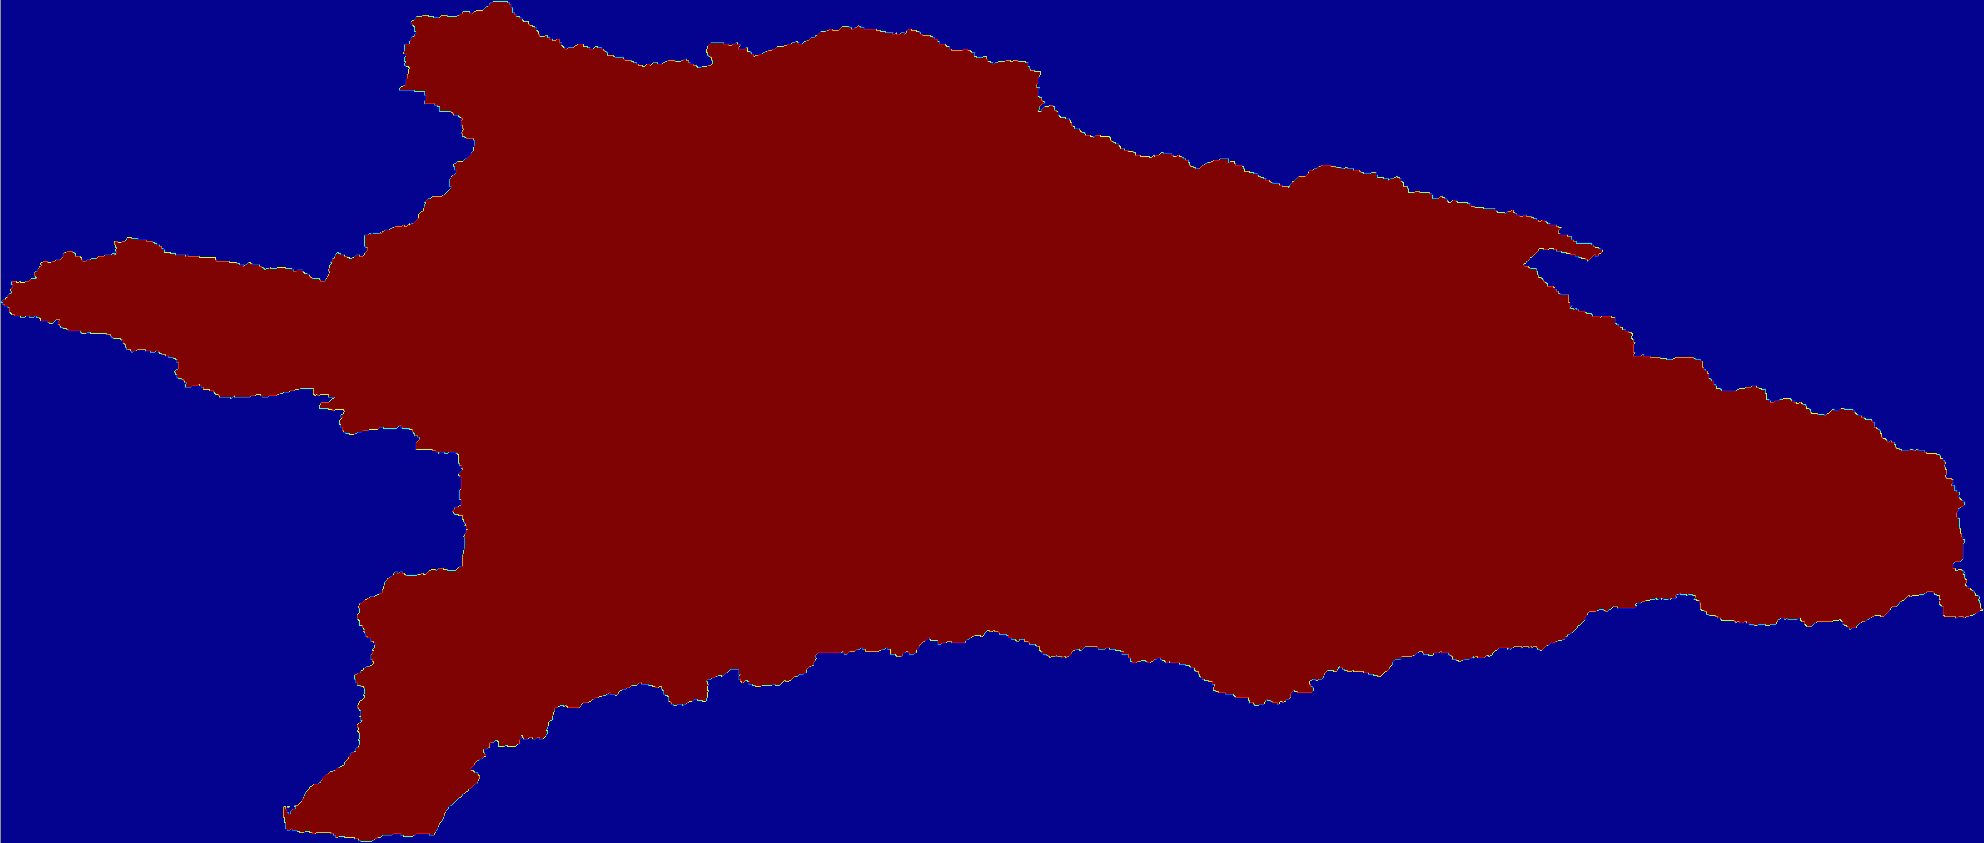
\includegraphics[width=5.5in]{figures/Oxnard_SearchDomain.png}   
            \caption{Oxnard Region Search Domain (Filled in Red)}
            \label{fig:Odomain}
            \end{center}
        \end{figure}
        
    \subsection{Destination Search Inputs}
    
Here the three key inputs to the Oxnard reuse destination search process are shown. A cursory visual inspection of these three layers reveals that there is an obvious band of continuously high suitability stretching from the foot of the basin (at the lower left) along its lower portion nearly across its breadth (to the lower right). This corridor is flat low lying river bed. It possesses a highly permeable surface geology, a very shallow slope profile, and relatively low intensity land use applications, as such, its composite suitability is very high and likely to contain the ultimate destination site for the hypothetical reuse system. 
    
        \begin{figure}[!h]
            \begin{center}
            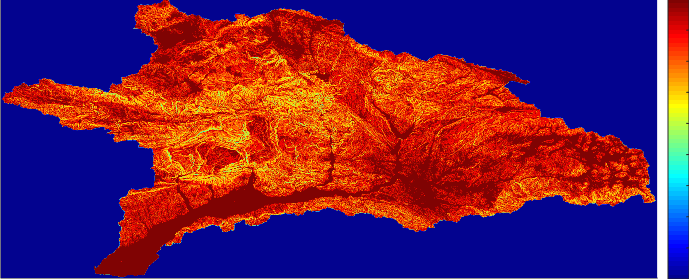
\includegraphics[width=5.5in]{figures/Oxnard_Search_Slope.png}   
            \caption{Oxnard Region Destination Search Inputs: Slope Score (Blue:Low, Red:High)}
            \label{fig:Odsinputs_slope}
            \end{center}
        \end{figure}
        
        \begin{figure}[!h]
            \begin{center}
            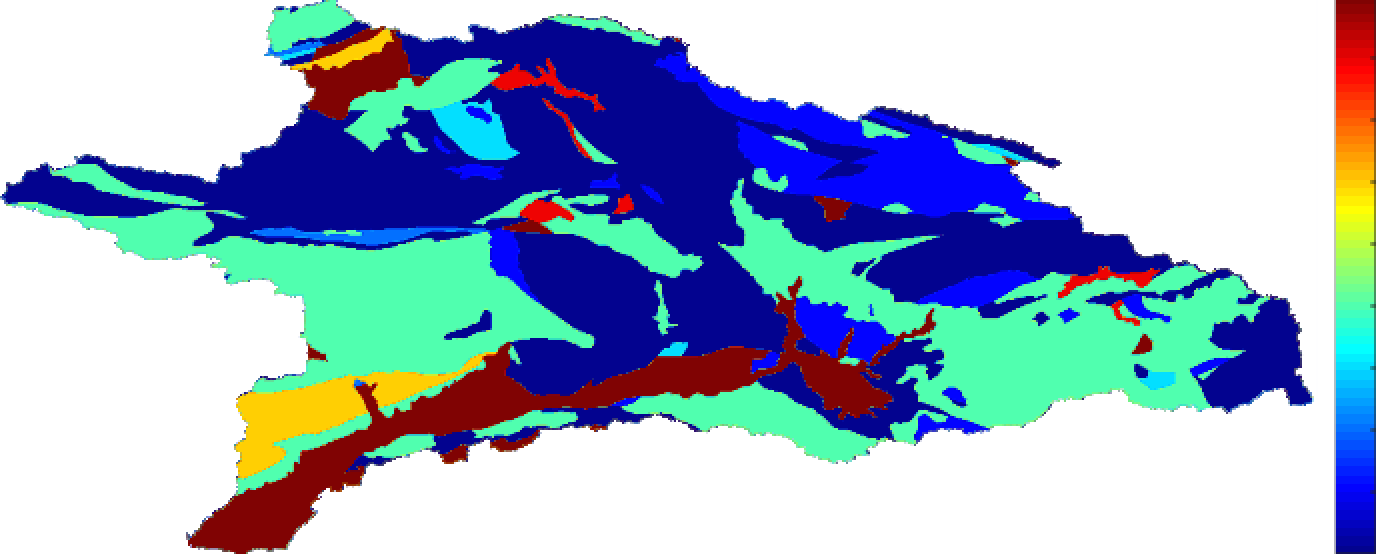
\includegraphics[width=5.5in]{figures/Oxnard_Search_Geology.png}   
            \caption{Oxnard Region Destination Search Inputs: Geology Score (Blue:Low, Red:High)}
            \label{fig:Odsinputs_geology}
            \end{center}
        \end{figure}
    
        \begin{figure}[!h]
            \begin{center}
            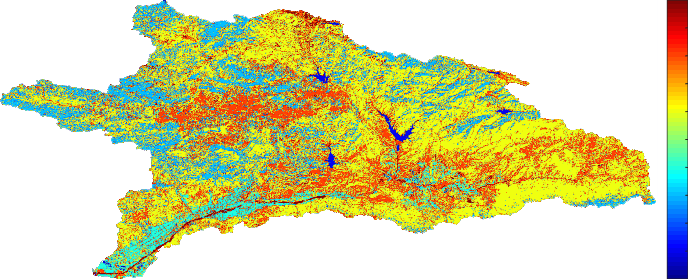
\includegraphics[width=5.5in]{figures/Oxnard_Search_Landuse.png}   
            \caption{Oxnard Region Destination Search Inputs: Landuse Score (Blue:Low, Red:High)}
            \label{fig:Odsinputs_landuse}
            \end{center}
        \end{figure}
    
    \subsection{Destination Search Outputs}
    
        \begin{figure}[!h]
            \begin{center}
            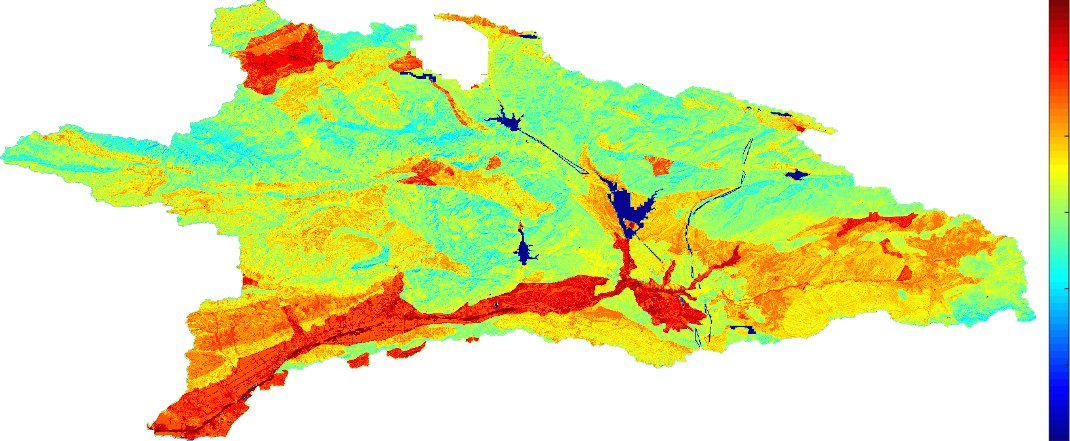
\includegraphics[width=5.5in]{figures/Oxnard_Search_Composite.png}   
            \caption{Oxnard Region Destination Search Outputs: Composite Scores (Blue:Low, Red:High)}
            \label{fig:Odsoutputs_comp}
            \end{center}
        \end{figure}
        
        \begin{figure}[!h]
            \begin{center}
            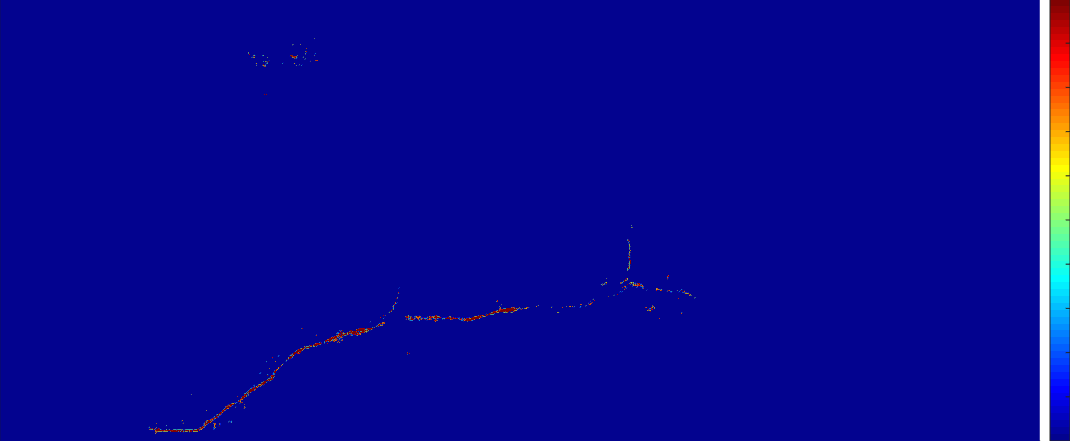
\includegraphics[width=5.5in]{figures/Oxnard_Search_Output.png}   
            \caption{Oxnard Region Destination Search Outputs: Candidate Regions}
            \label{fig:Odsoutputs_cand}
            \end{center}
        \end{figure}

    \subsection{Proposed Corridor Endpoints}
    
    \begin{itemize}
      \setlength{\itemsep}{0cm}
      \setlength{\parskip}{0cm}
        \item Start Location: $(656,236)$
        \item End Destination: $(513,532)$
        \item Shortest Euclidean Path Distance: $32,873$ $m$ ($32$ $km$)
    \end{itemize}
    
        \begin{figure}[!h]
            \begin{center}
            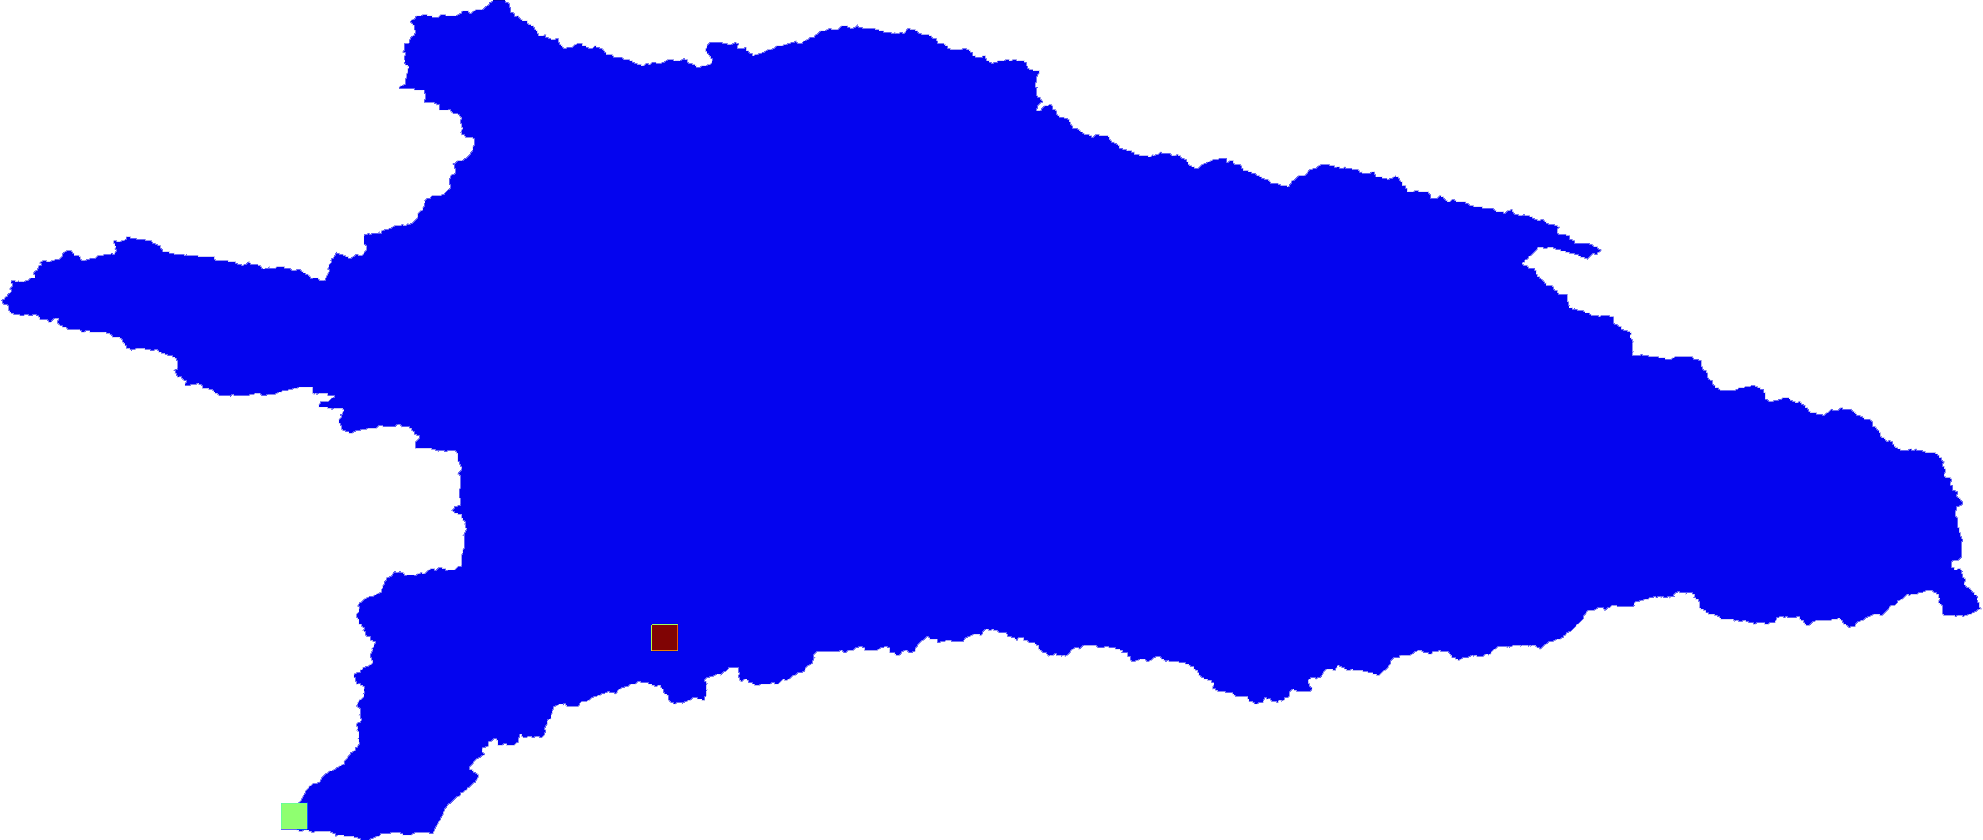
\includegraphics[width=5.5in]{figures/Oxnard_Endpoints.png}   
            \caption{Oxnard Region Proposed Corridor Endpoints}
            \label{fig:Oendpoints}
            \end{center}
        \end{figure}
            
    \subsection{Proposed Objective Layers}

        \begin{figure}[!h]
            \begin{center}
            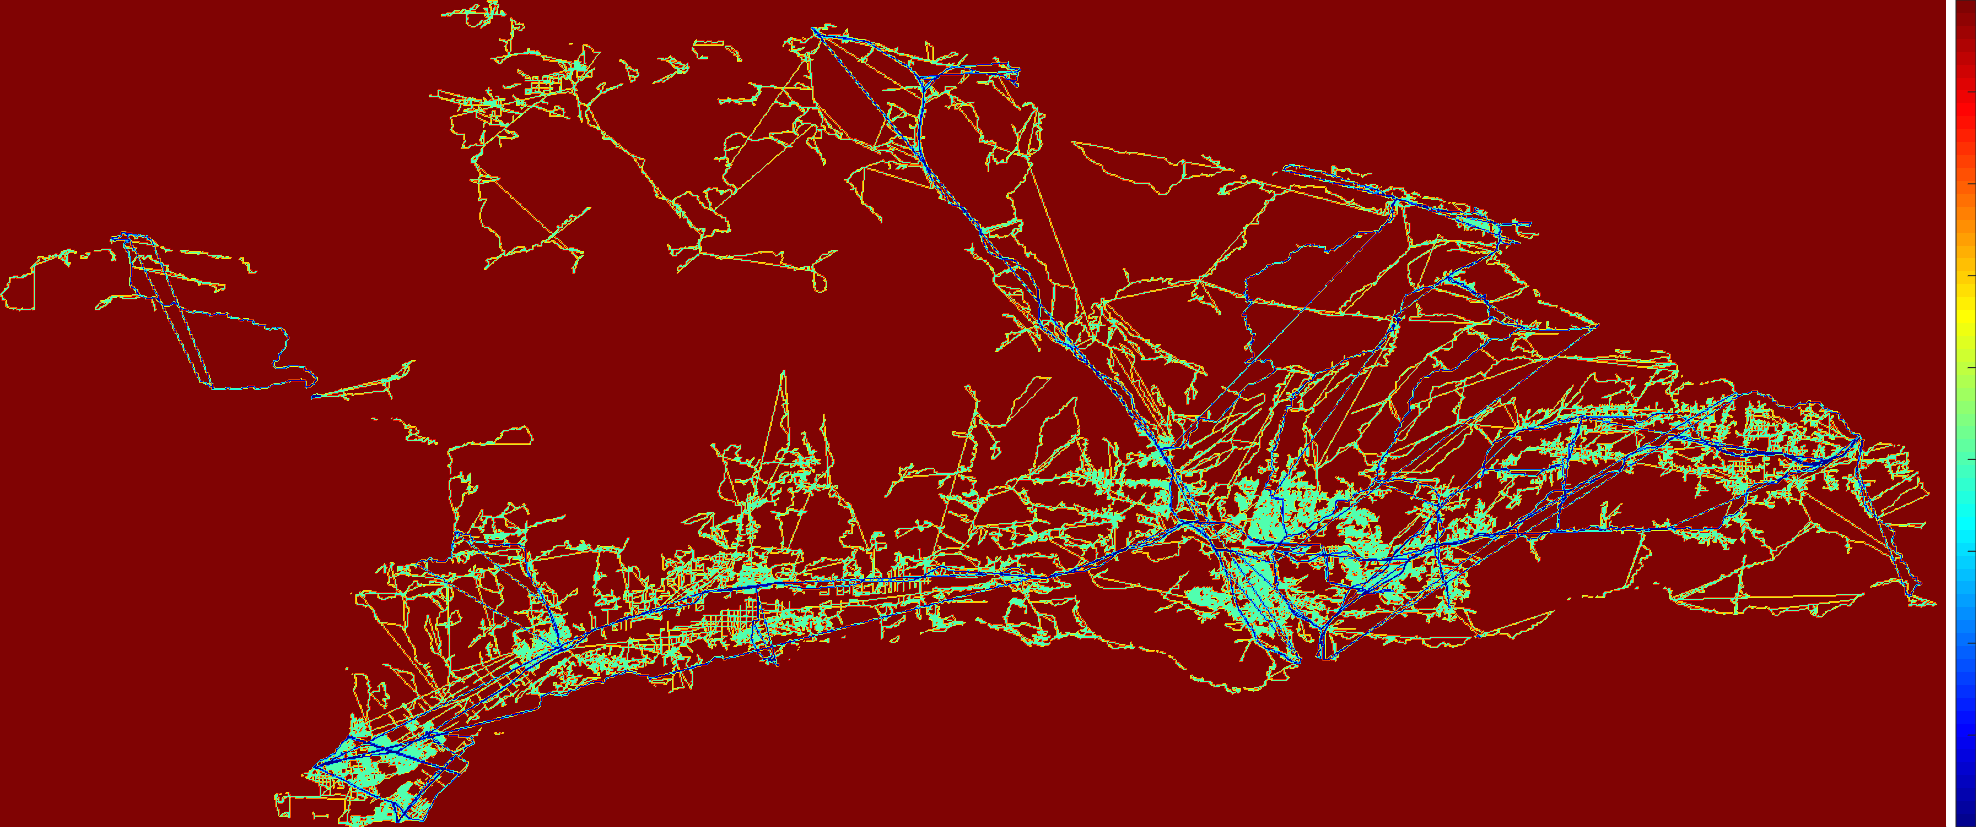
\includegraphics[width=5.5in]{figures/Oxnard_AccessibilityScore.png}   
            \caption{Oxnard Region Accessibility Based Objective Scores (Blue:Low, Red:High)}
            \label{fig:Oaccessibilty}
            \end{center}
        \end{figure}

        \begin{figure}[!h]
            \begin{center}
            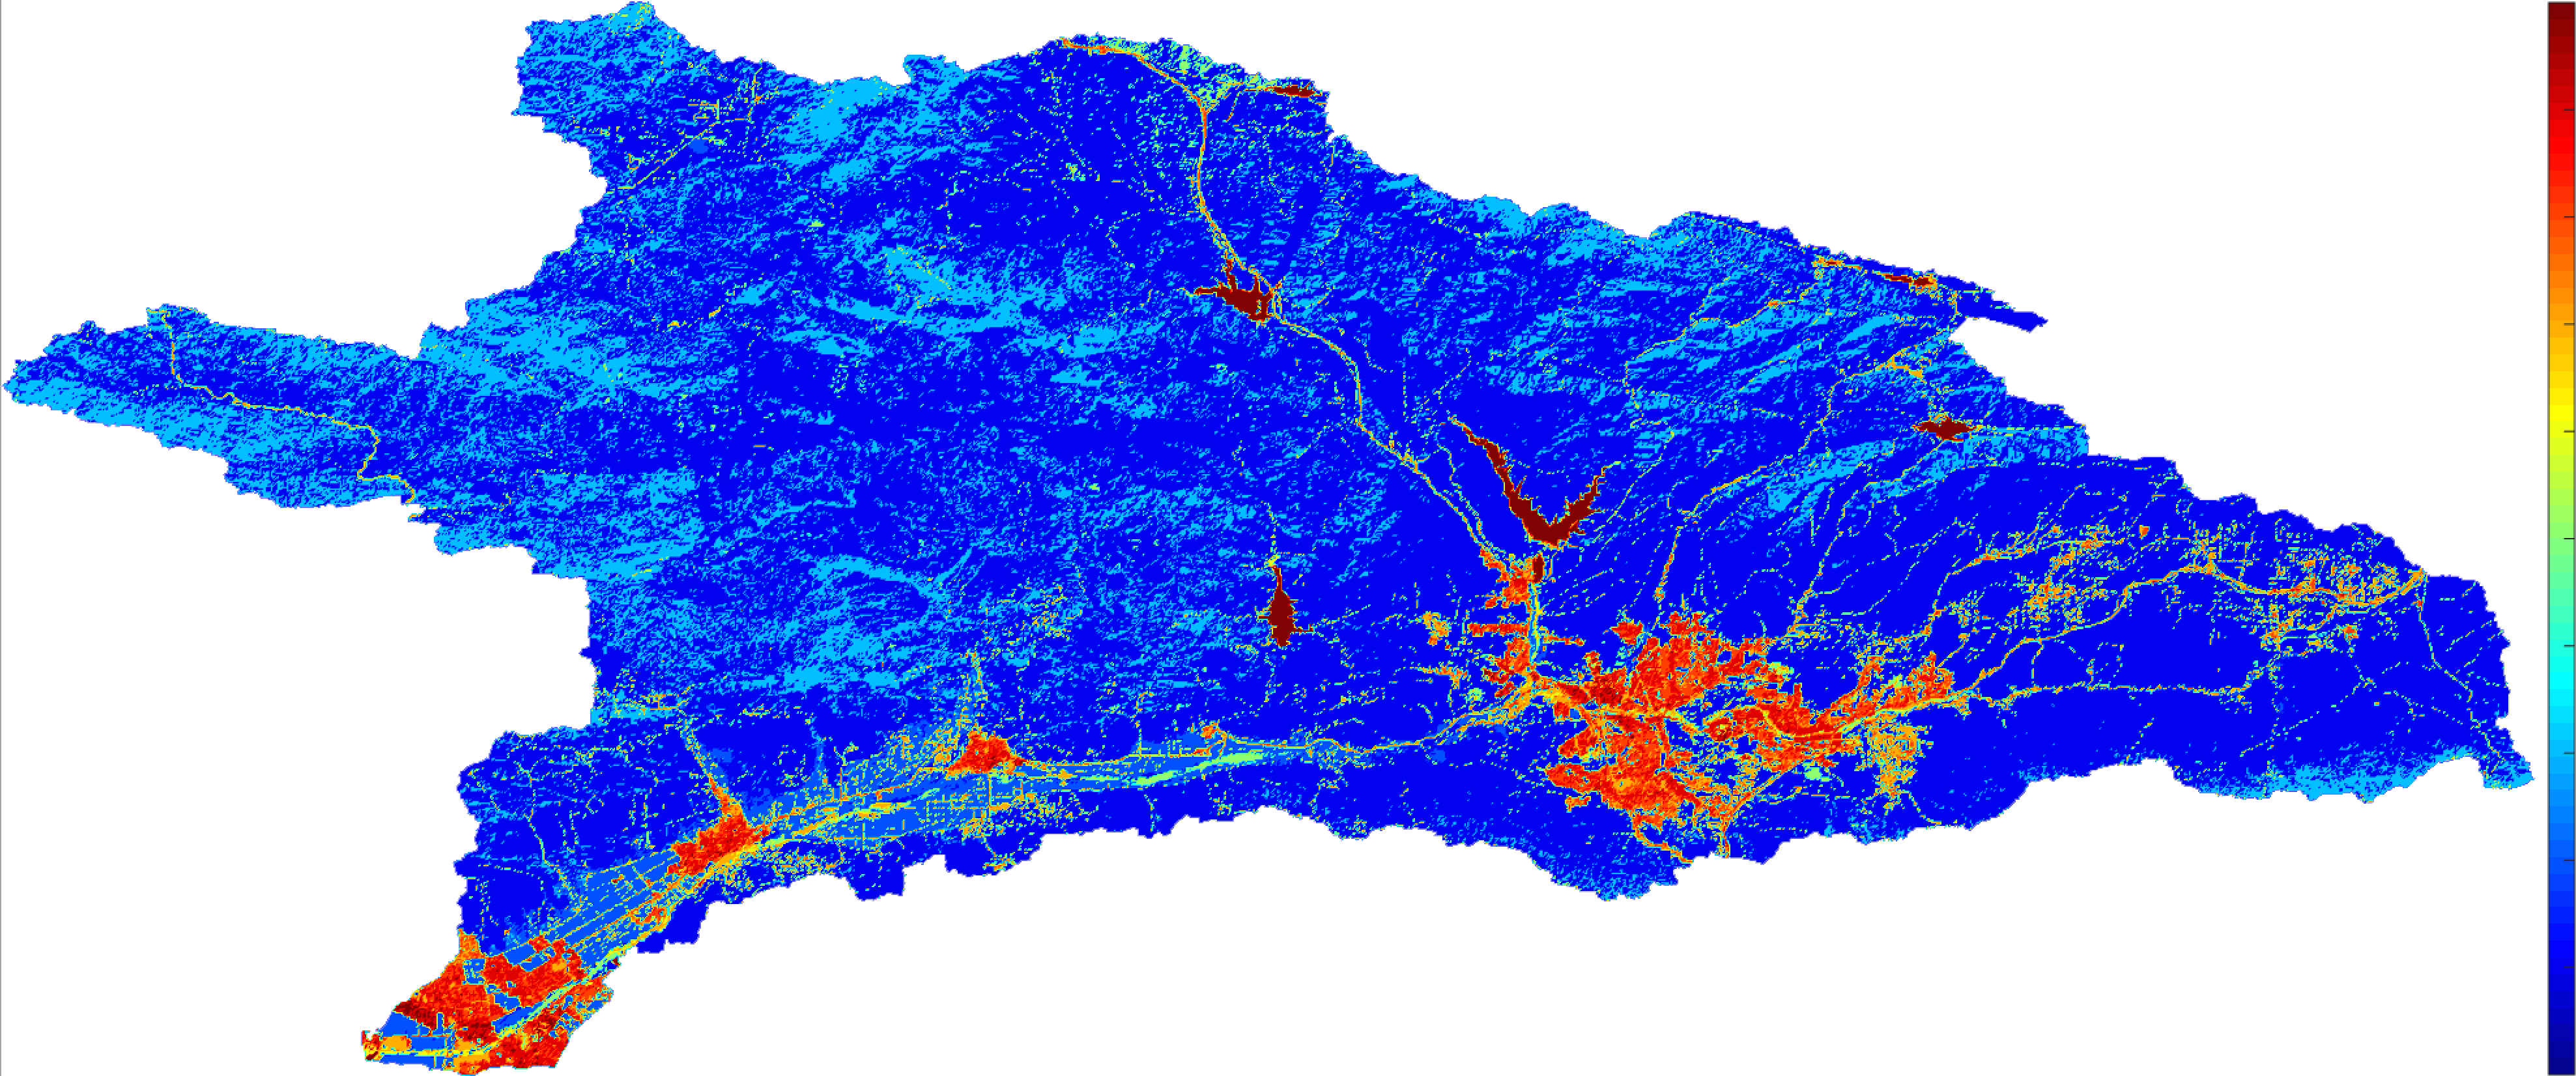
\includegraphics[width=5.5in]{figures/Oxnard_DisturbanceScore.png}   
            \caption{Oxnard Region Land Use Based Disturbance Objective Scores (Blue:Low, Red:High)}
            \label{fig:Odisturbance}
            \end{center}
        \end{figure}
        
        \begin{figure}[!h]
            \begin{center}
            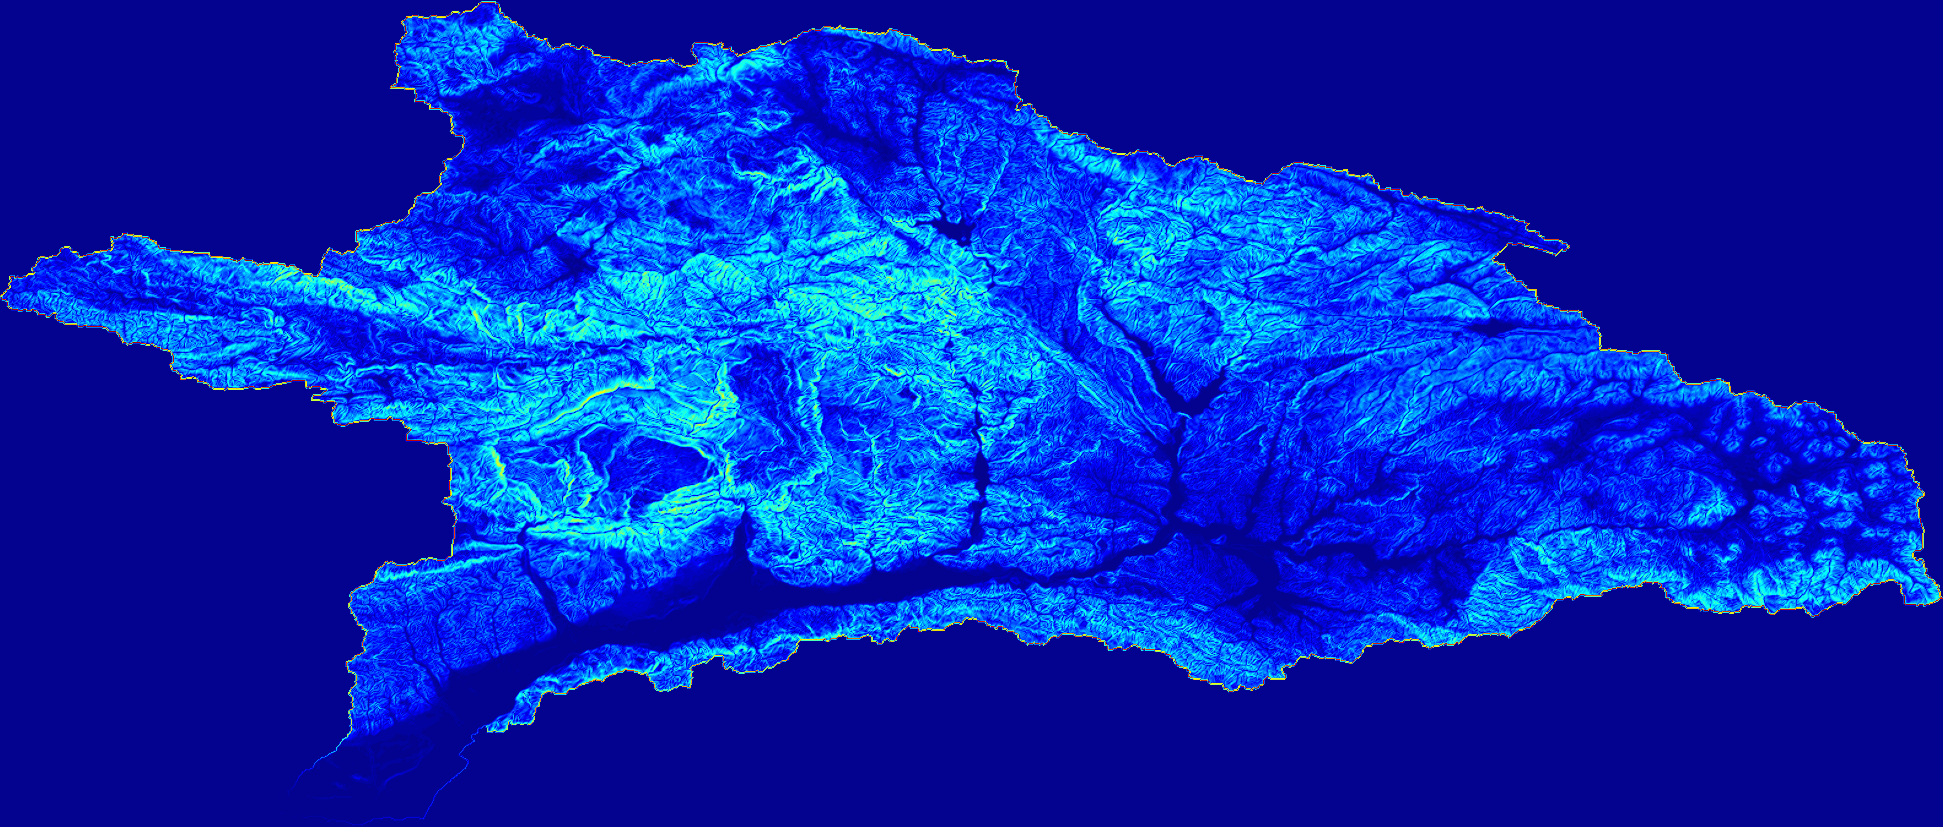
\includegraphics[width=5.5in]{figures/Oxnard_SlopeScore.png}   
            \caption{Oxnard Region Slope Based Objective Scores (Blue:Low, Red:High)}
            \label{fig:Oslope}
            \end{center}
        \end{figure}
        
    \subsection{Proposed Corridor Solutions}
    
        \begin{figure}[!h]
            \begin{center}
            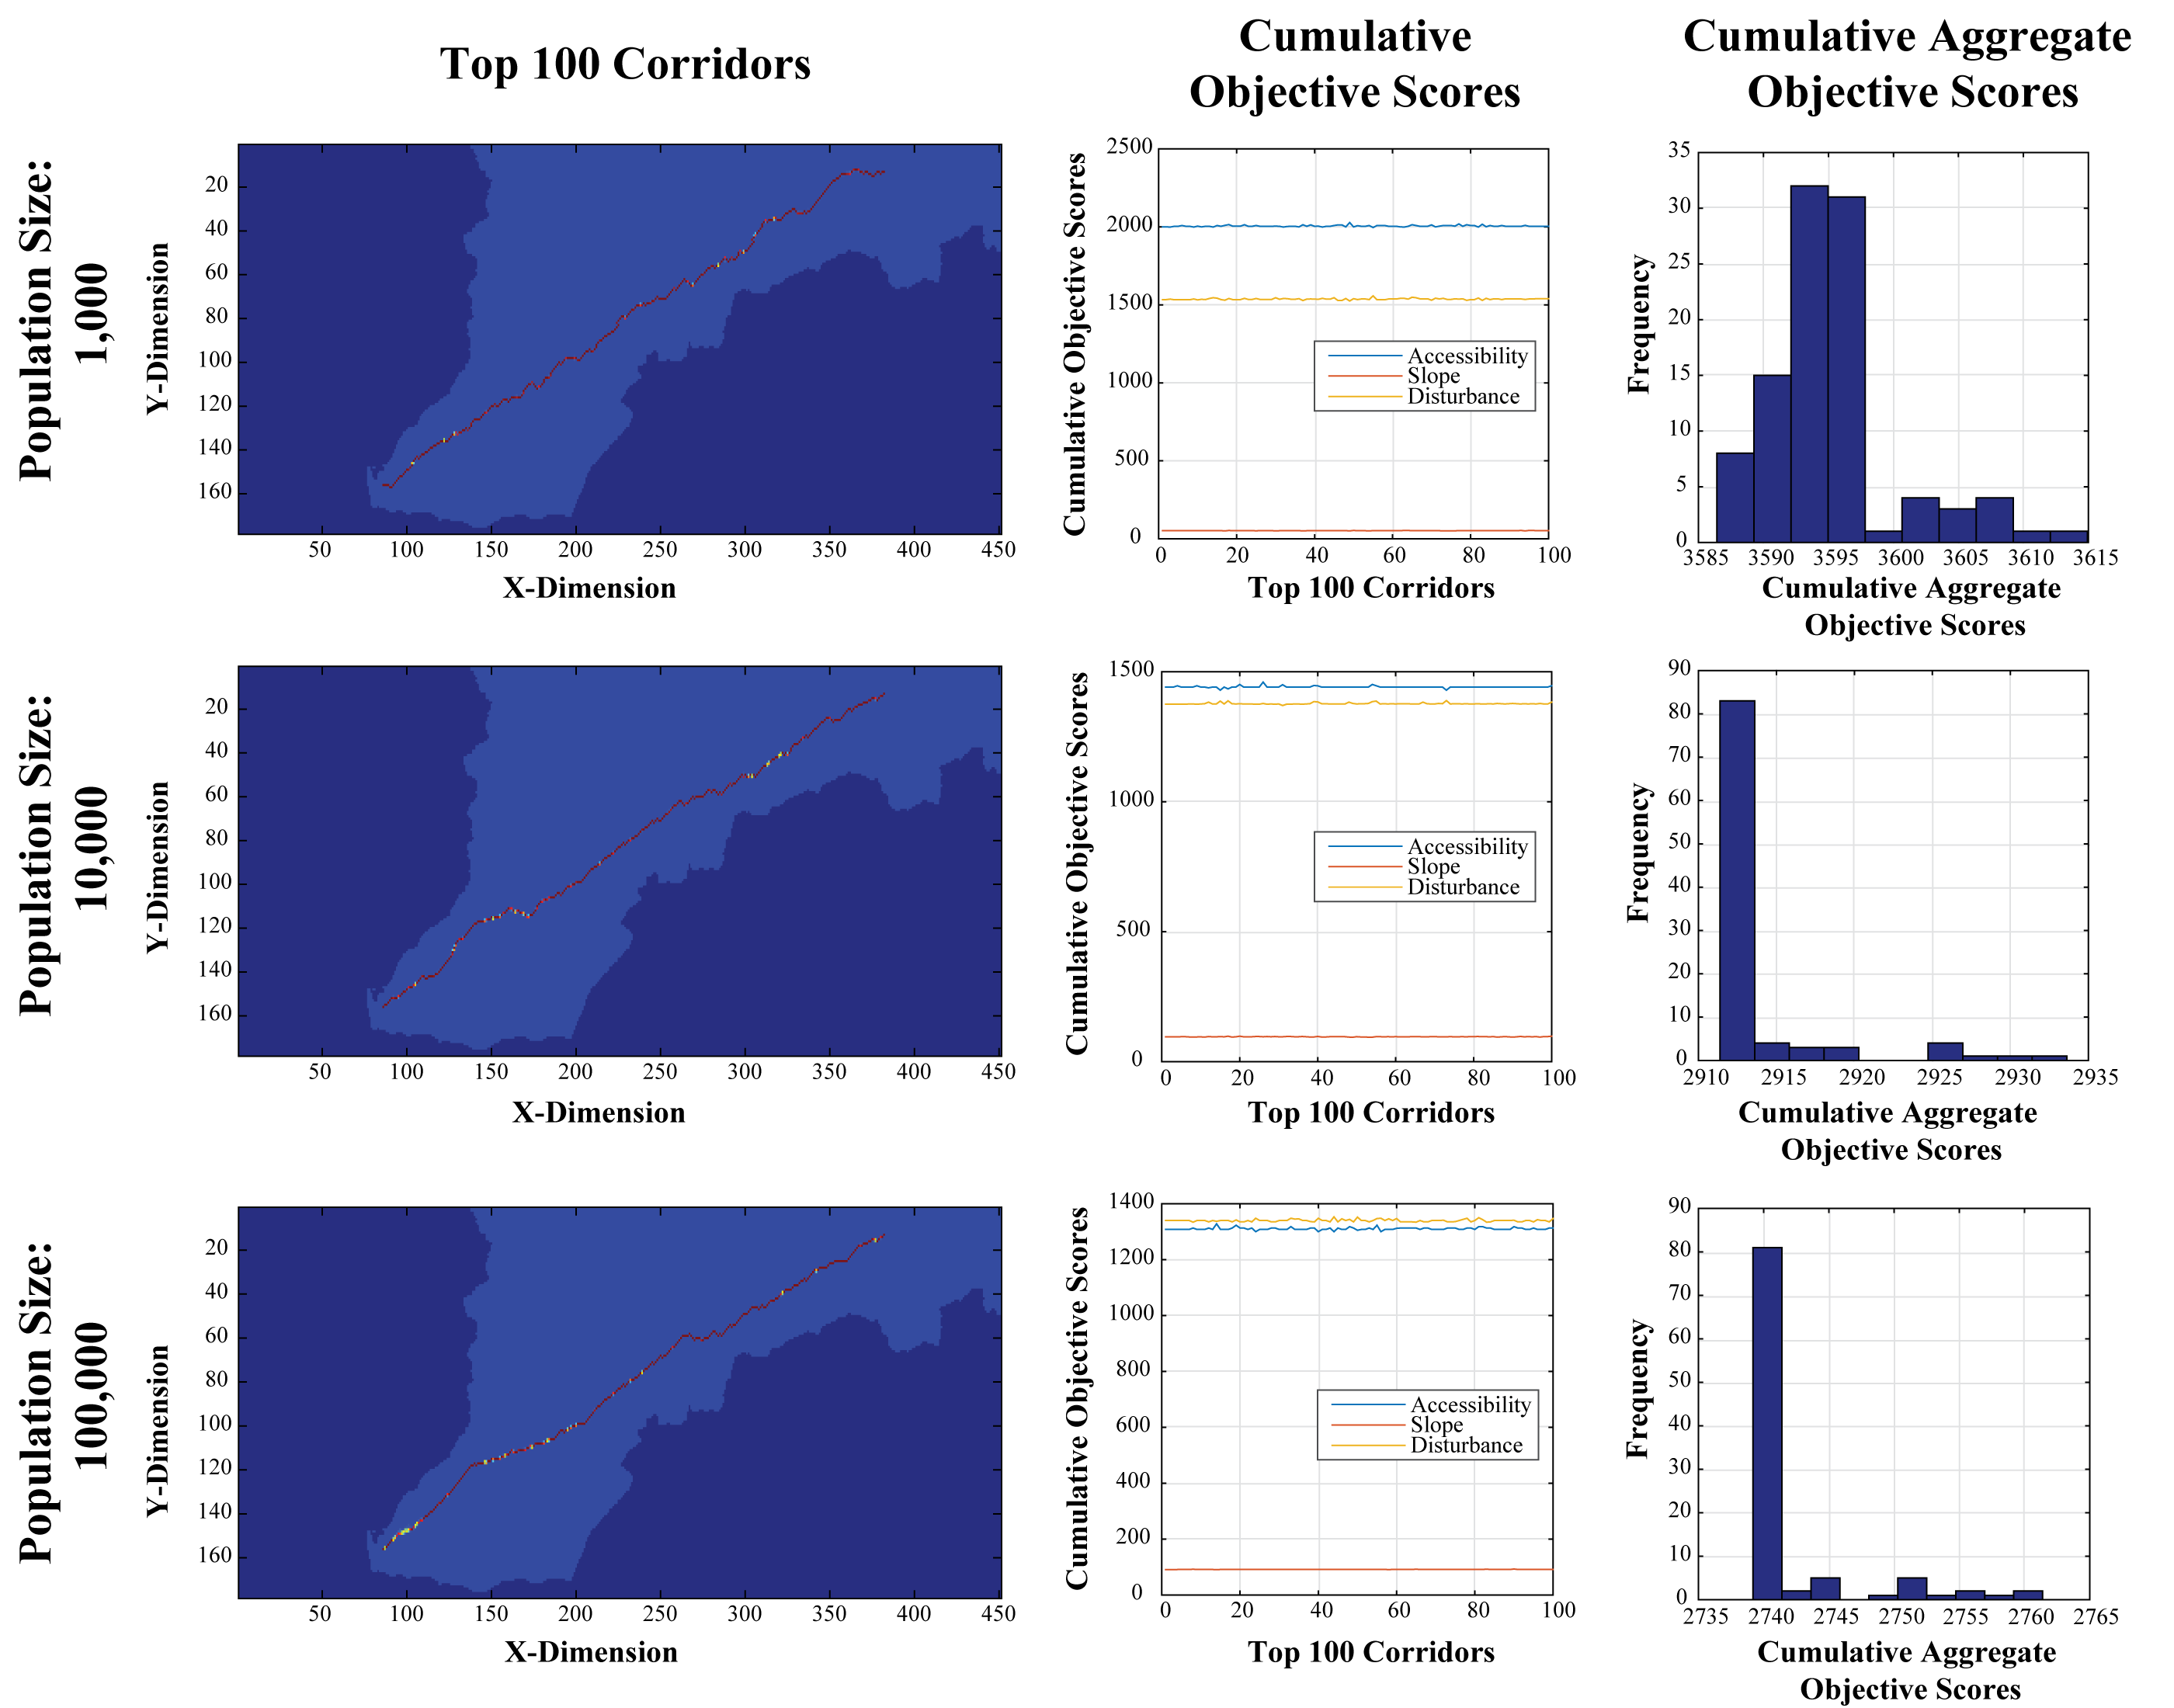
\includegraphics[width=6in]{figures/Oxnard_PathwayResults.png}   
            \caption{Oxnard Region Corridor Analysis Results}
            \label{fig:Oresults}
            \end{center}
        \end{figure}

        \begin{figure}[!h]
            \begin{center}
            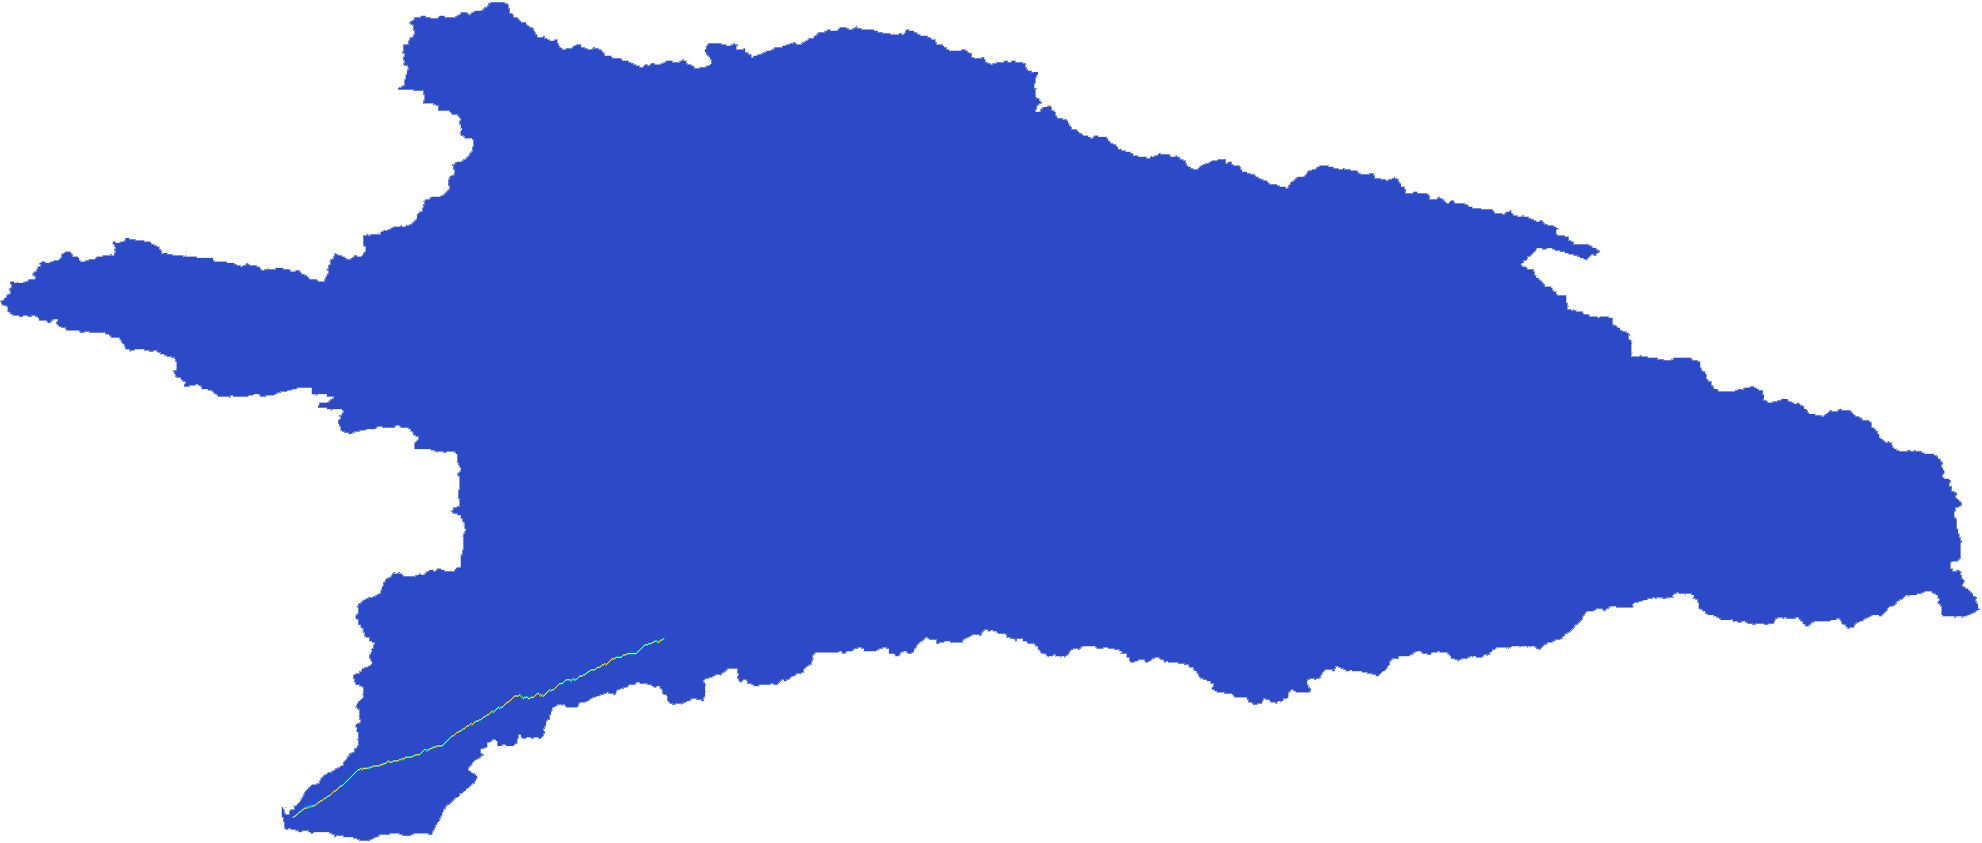
\includegraphics[width=5.5in]{figures/Oxnard_PathwayLarge.png}   
            \caption{Oxnard Region Top 100 Corridors (Pop Size: 100,000) Basin Wide Overview}
            \label{fig:OsolutionOverview}
            \end{center}
        \end{figure}
        
        \begin{figure}[!h]
            \begin{center}
            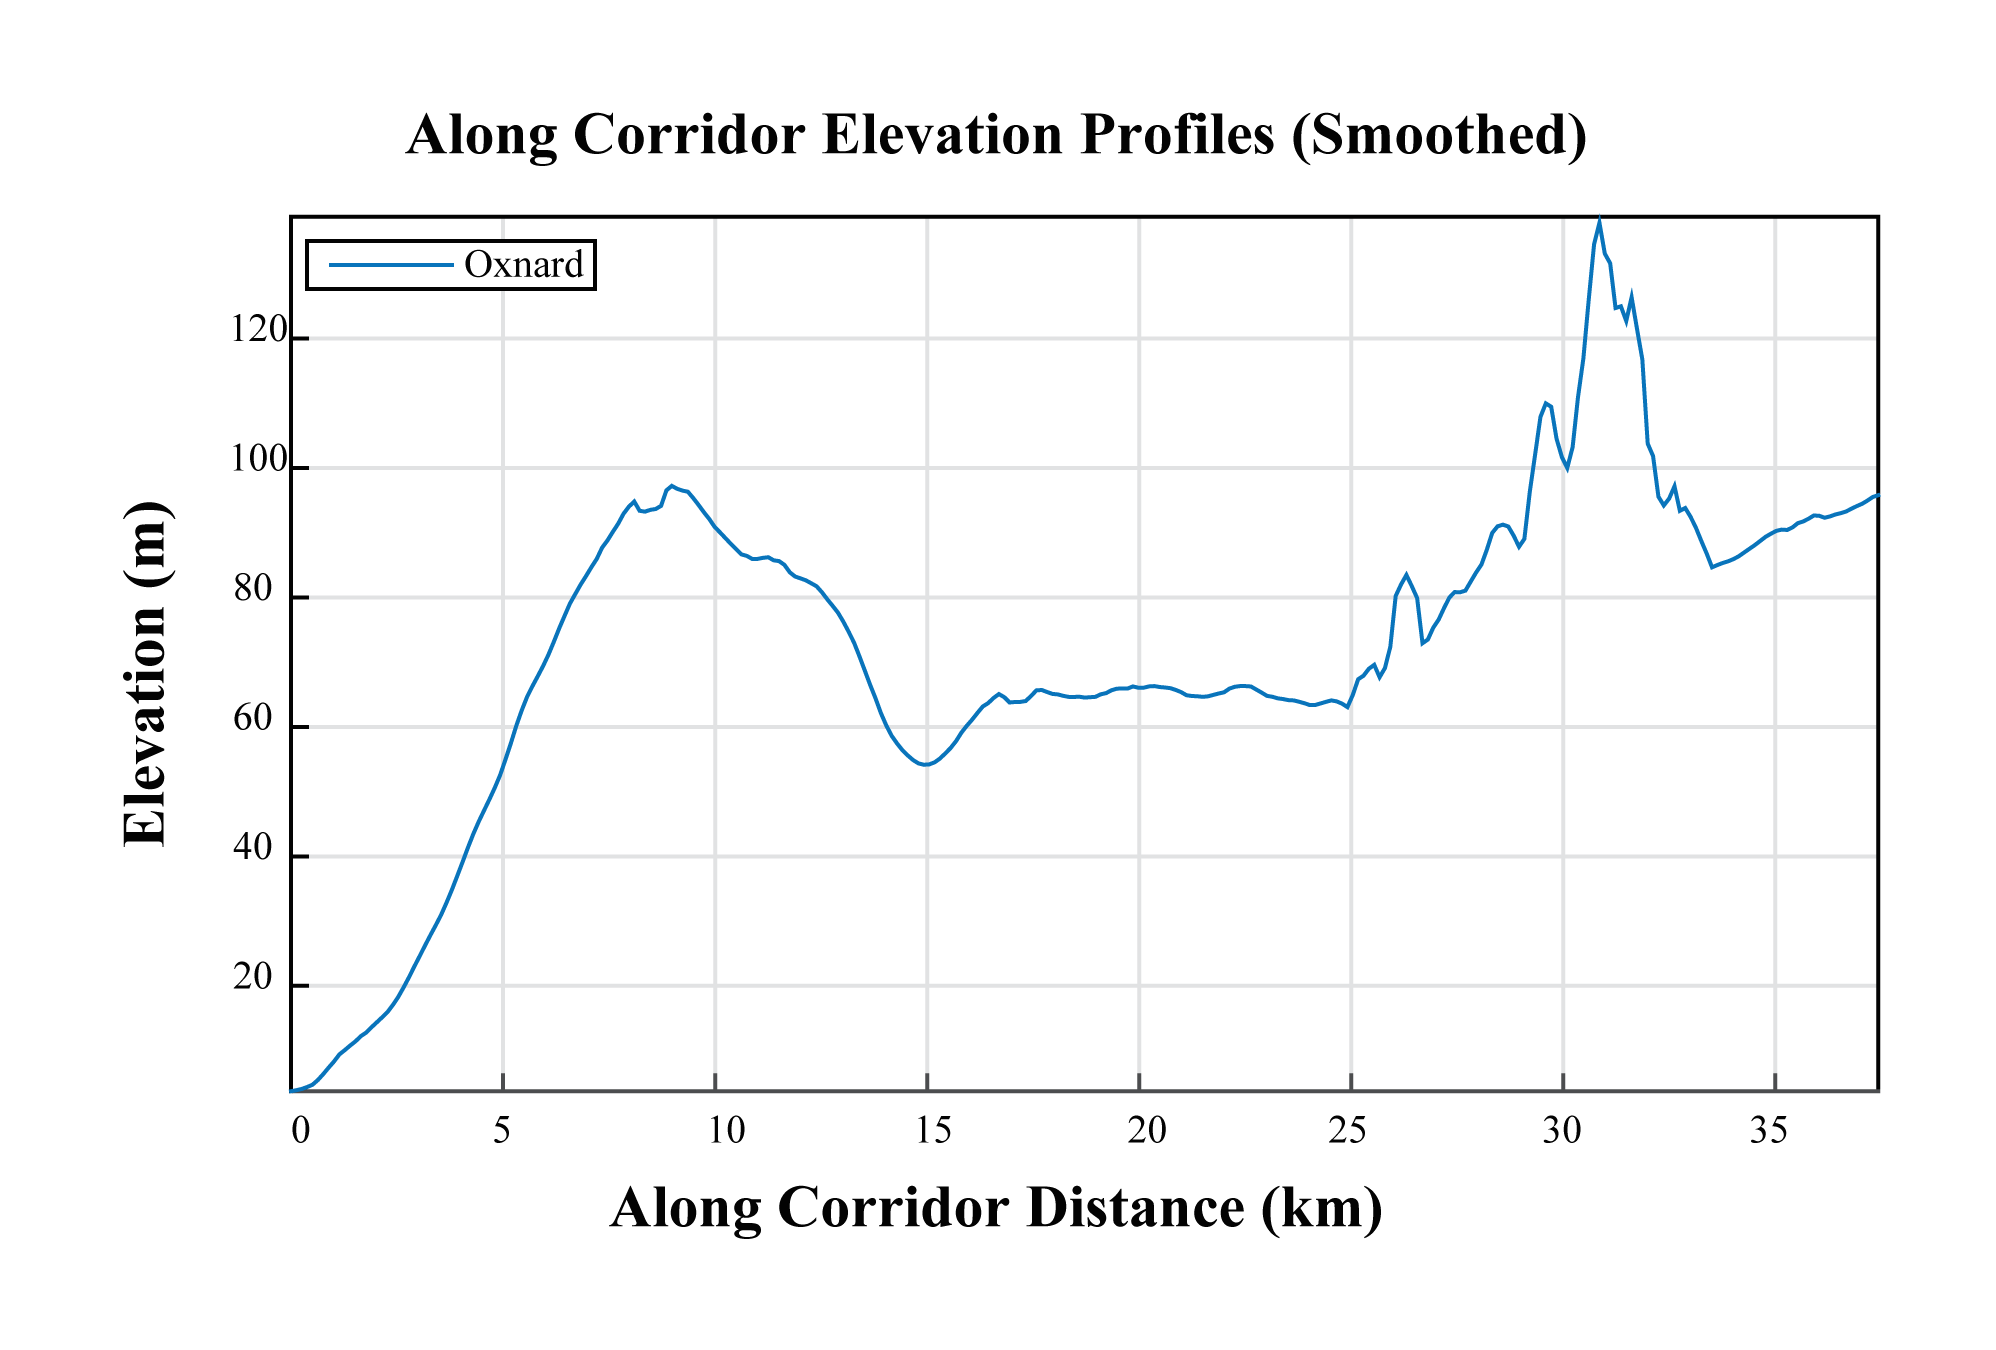
\includegraphics[width=5.5in]{figures/Oxnard_Elevation_Profile.png}
            \caption{Oxnard Region Proposed Corridor Elevation Profile}
            \label{fig:OelevationProfile}
            \end{center}
        \end{figure}
    
    \subsection{Anticipated Distribution of Life Cycle Energy Usages and Net Water Savings}    
    
\clearpage    
    
\section{San Diego Region}

    \subsection{Regional Context}
    
    \begin{itemize}
      \setlength{\itemsep}{0cm}
      \setlength{\parskip}{0cm}
        \item HUC-8 Code: $18070304$
        \item Total Area: $4,338.1$ $km^2$
        \item Maximum Elevation: $1,977$ $m$
        \item Minimum Elevation: $-0.7$ $m$
        \item Mean Slope: $9.38$ $\%$
        \item Standard Deviation of Slope: $8.77$ $\%$
        \item Dominant Soil Composition: Hydrologic Soil Group - B: $10-20\%$ clay, $50-90\%$ sand, $35\%$ rock fragments
    \end{itemize}
    
        \begin{figure}[!h]
            \begin{center}
            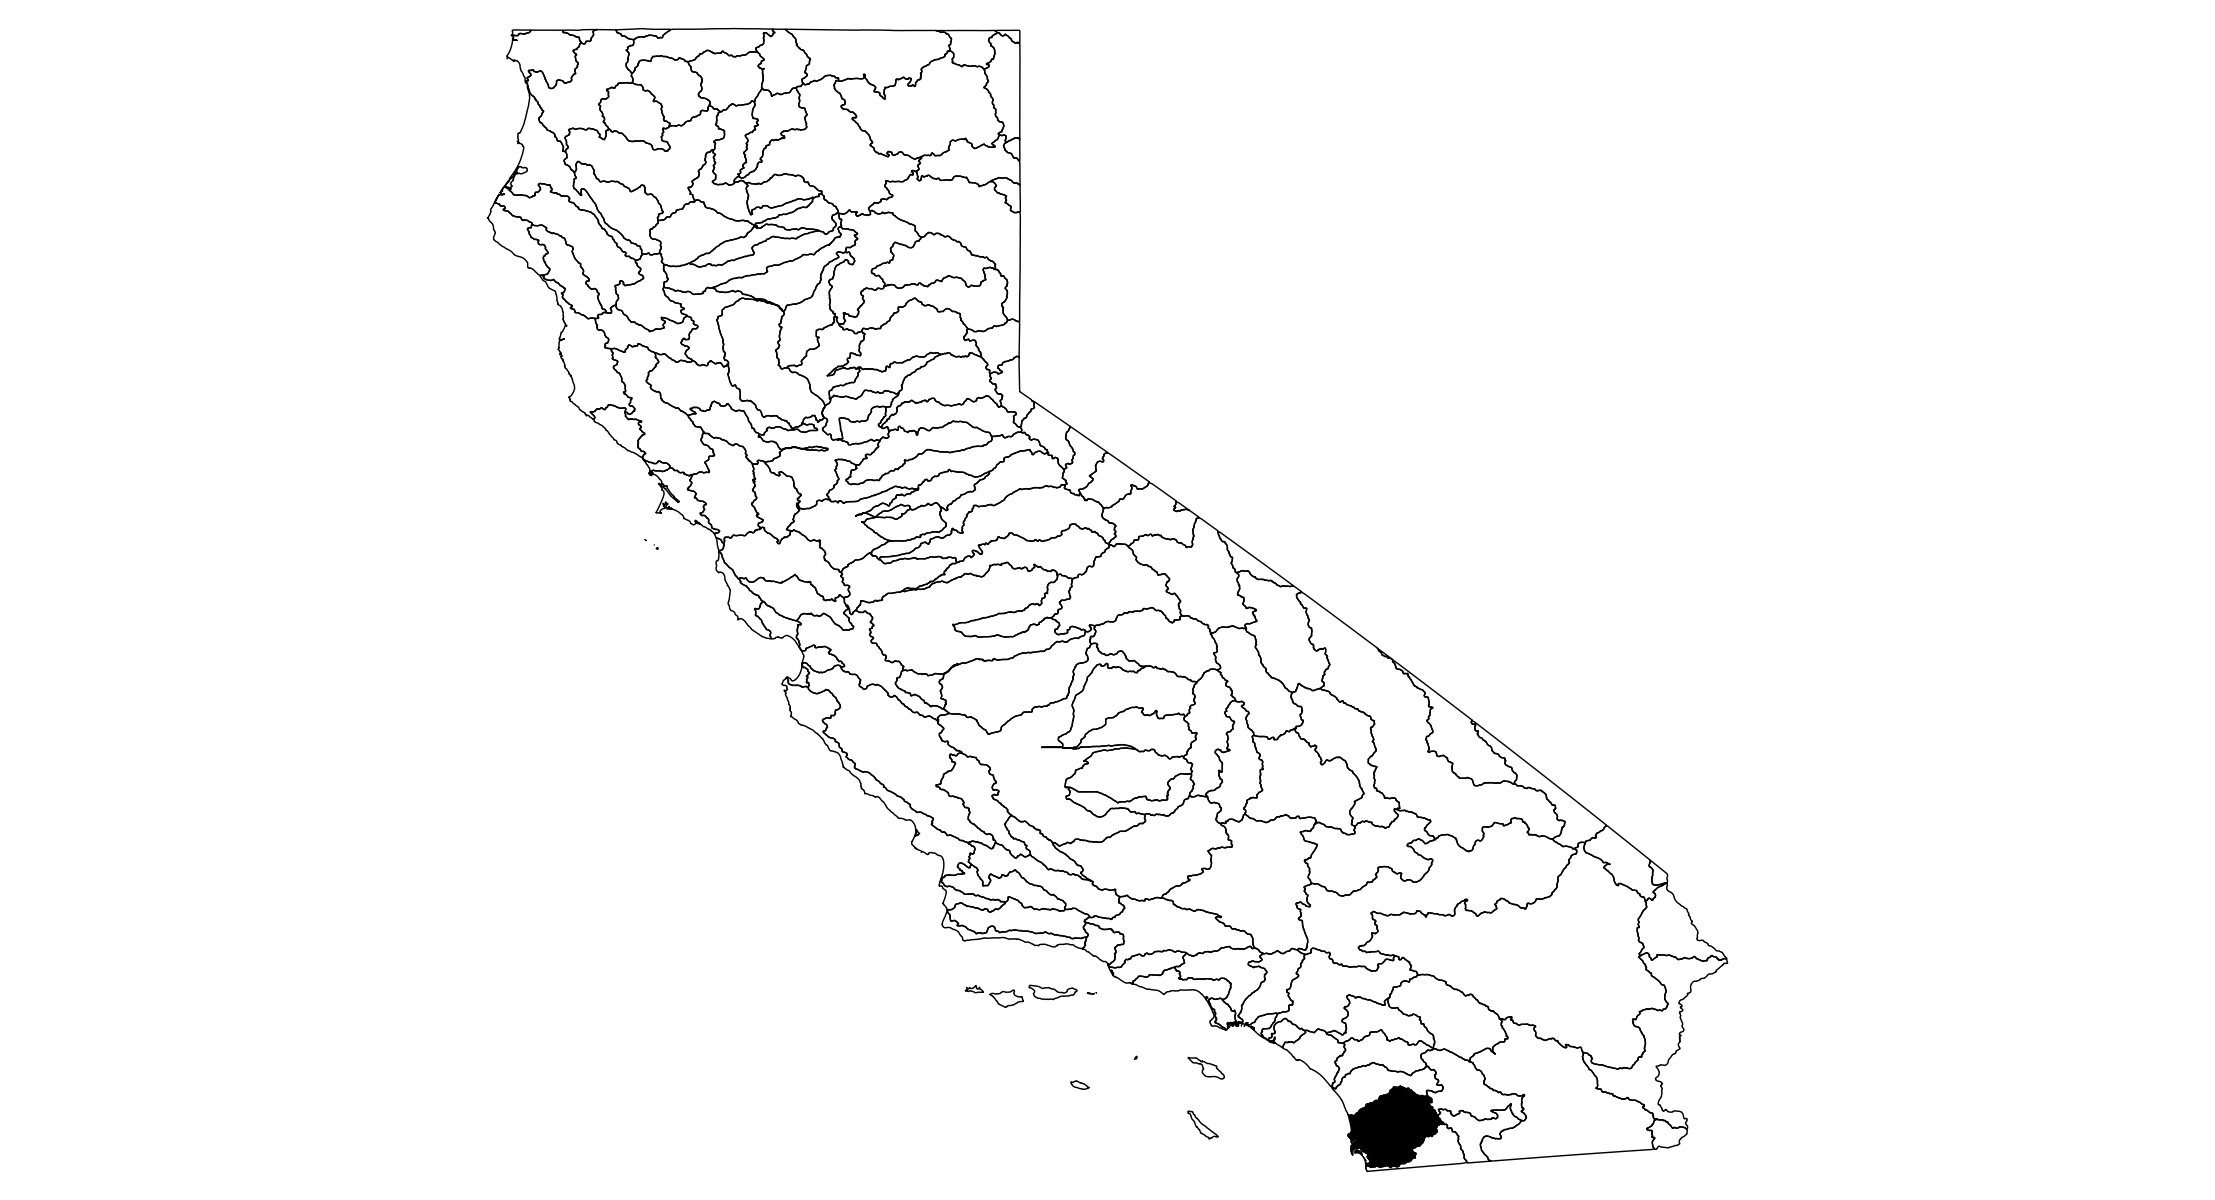
\includegraphics[width=5.5in]{figures/SanDiego_Overview.png}   
            \caption{San Diego Region Overview (Filled in Black)}
            \label{fig:SDoverview}
            \end{center}
        \end{figure}

    \subsection{Search Domain}
    
    \begin{itemize}
      \setlength{\itemsep}{0cm}
      \setlength{\parskip}{0cm}
        \item Grid Dimensions: $798$ $cells$ x $898$ $cells$
        \item Grid Cell Resolution: $100$ $m$ x $100$ $m$ ($1$ $ha$)
        \item Feasible Grid Cells: $433,808$ $cells$
    \end{itemize}
    
        \begin{figure}[!h]
            \begin{center}
            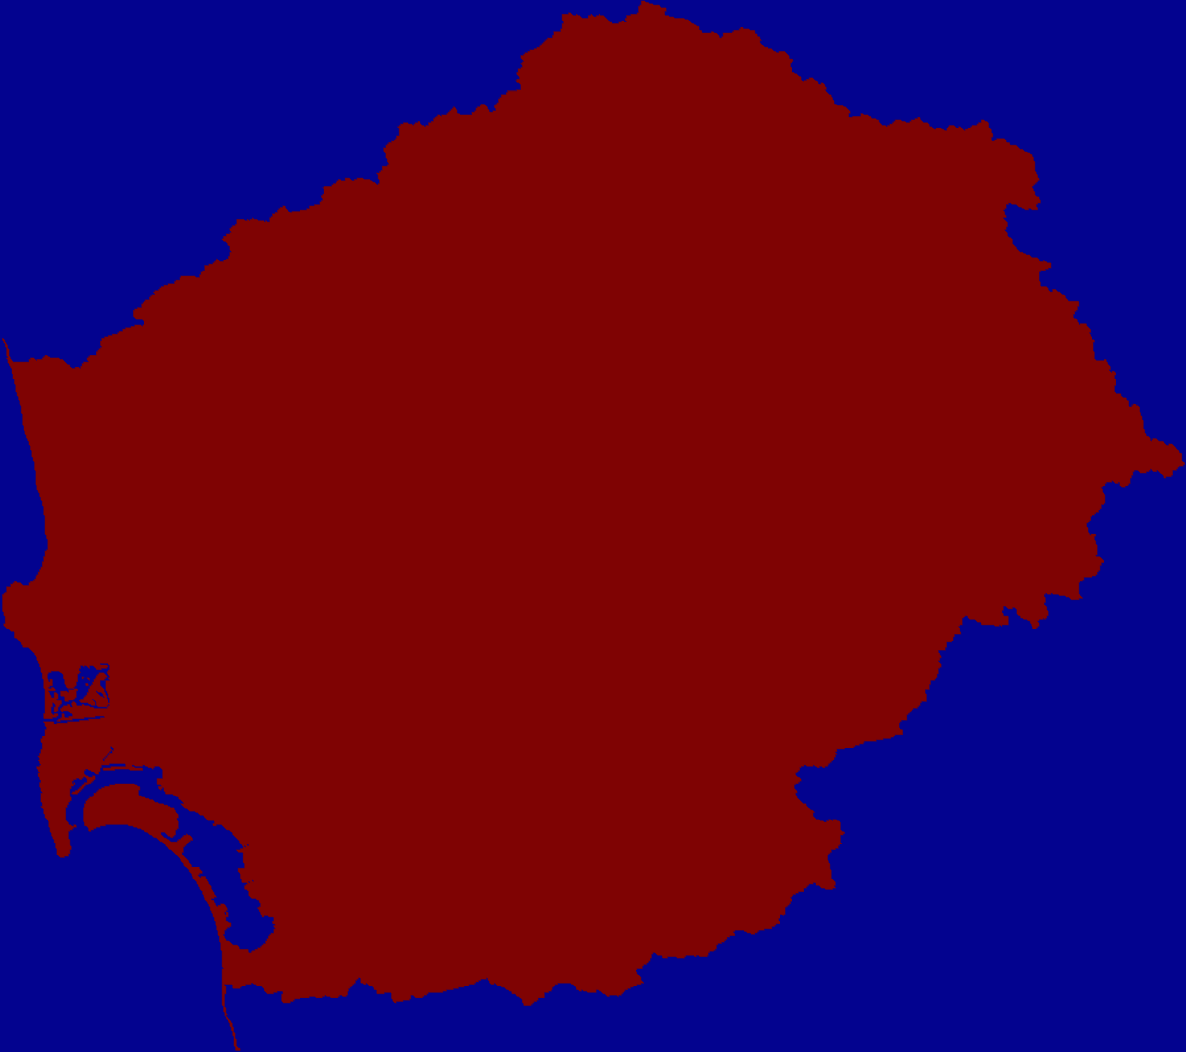
\includegraphics[width=5.5in]{figures/SanDiego_SearchDomain.png}   
            \caption{San Diego Region Search Domain (Filled in Red)}
            \label{fig:SDdomain}
            \end{center}
        \end{figure}

    \subsection{Proposed Corridor Endpoints}
    
    \begin{itemize}
      \setlength{\itemsep}{0cm}
      \setlength{\parskip}{0cm}
        \item Start Location: $(635,42)$
        \item End Destination: $(453,363)$    
        \item Shortest Euclidean Path Distance: $36,901$ $m$ ($36$ $km$)
    \end{itemize}
    
        \begin{figure}[!h]
            \begin{center}
            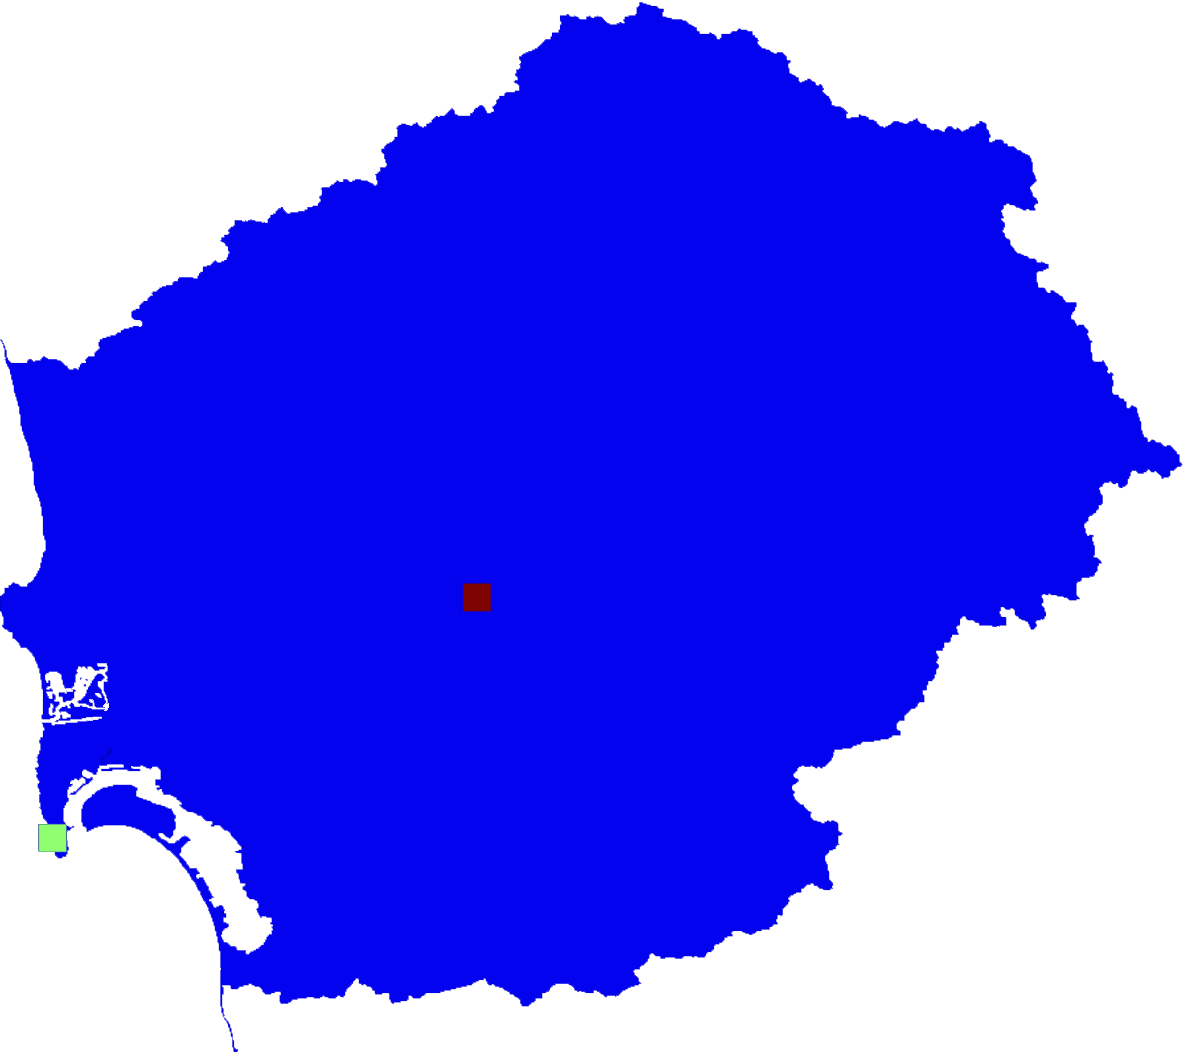
\includegraphics[width=5.5in]{figures/SanDiego_Endpoints.png}   
            \caption{San Diego Region Proposed Corridor Endpoints}
            \label{fig:SDendpoints}
            \end{center}
        \end{figure}

    \subsection{Proposed Objective Layers}

        \begin{figure}[!h]
            \begin{center}
            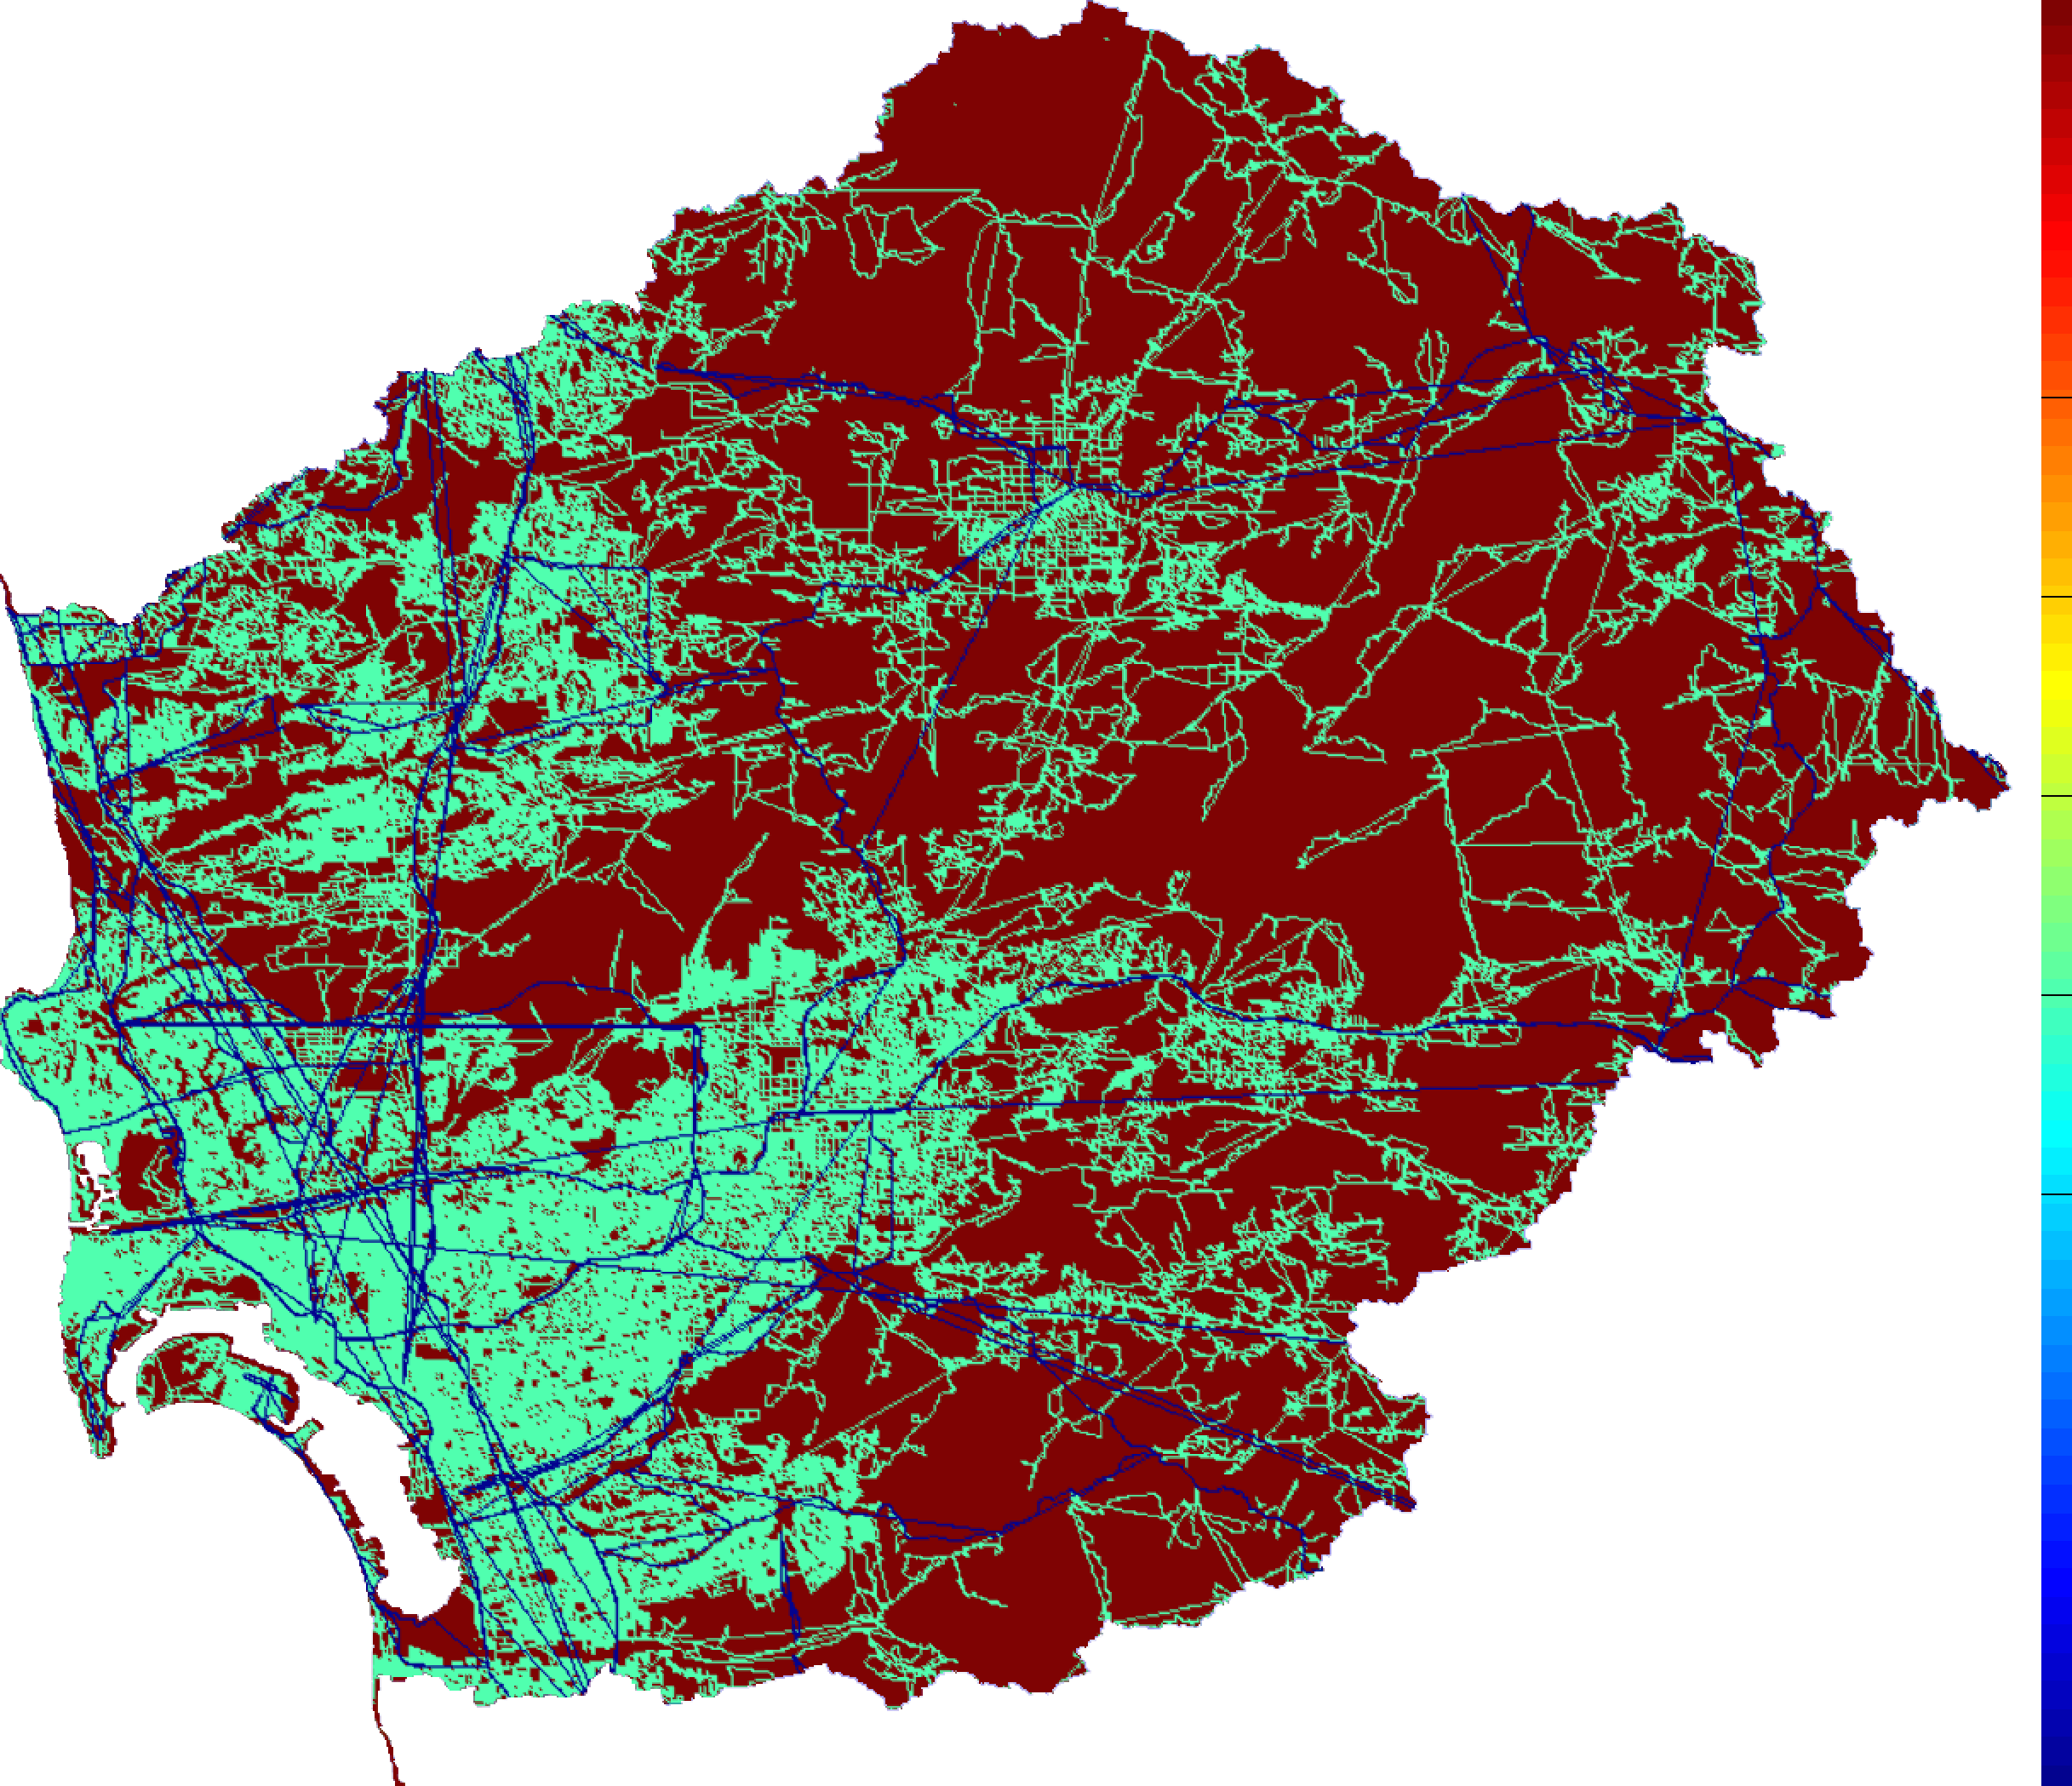
\includegraphics[width=5.5in]{figures/SanDiego_AccessibilityScore.png}   
            \caption{San Diego Region Accessibility Based Objective Scores (Blue:Low, Red:High)}
            \label{fig:SDaccessibilty}
            \end{center}
        \end{figure}

        \begin{figure}[!h]
            \begin{center}
            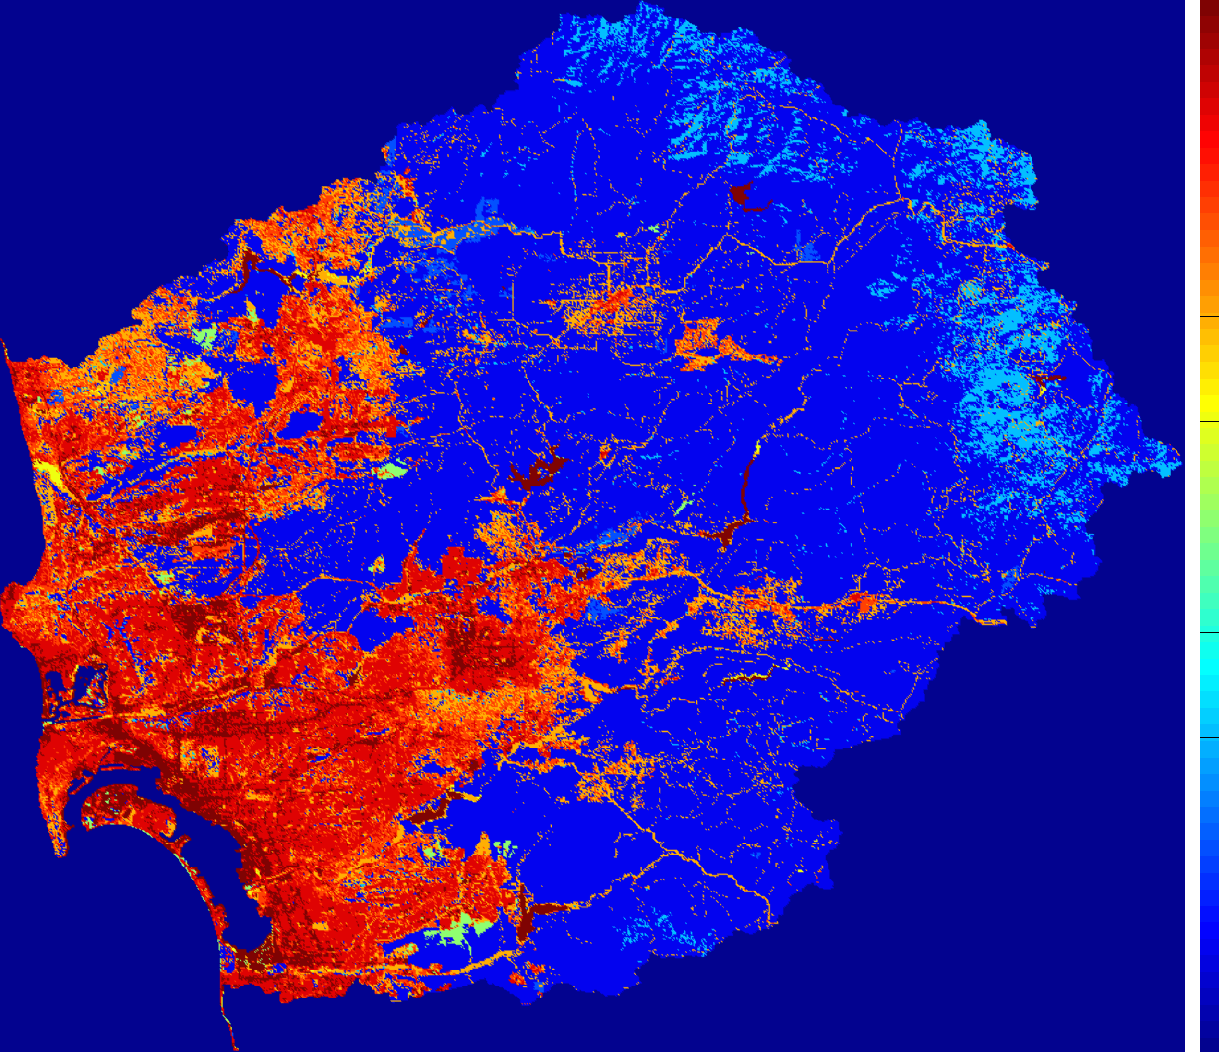
\includegraphics[width=5.5in]{figures/SanDiego_DisturbanceScore.png}   
            \caption{San Diego Region Land Use Disturbance Based Objective Scores (Blue:Low, Red:High)}
            \label{fig:SDdisturbance}
            \end{center}
        \end{figure}
        
        \begin{figure}[!h]
            \begin{center}
            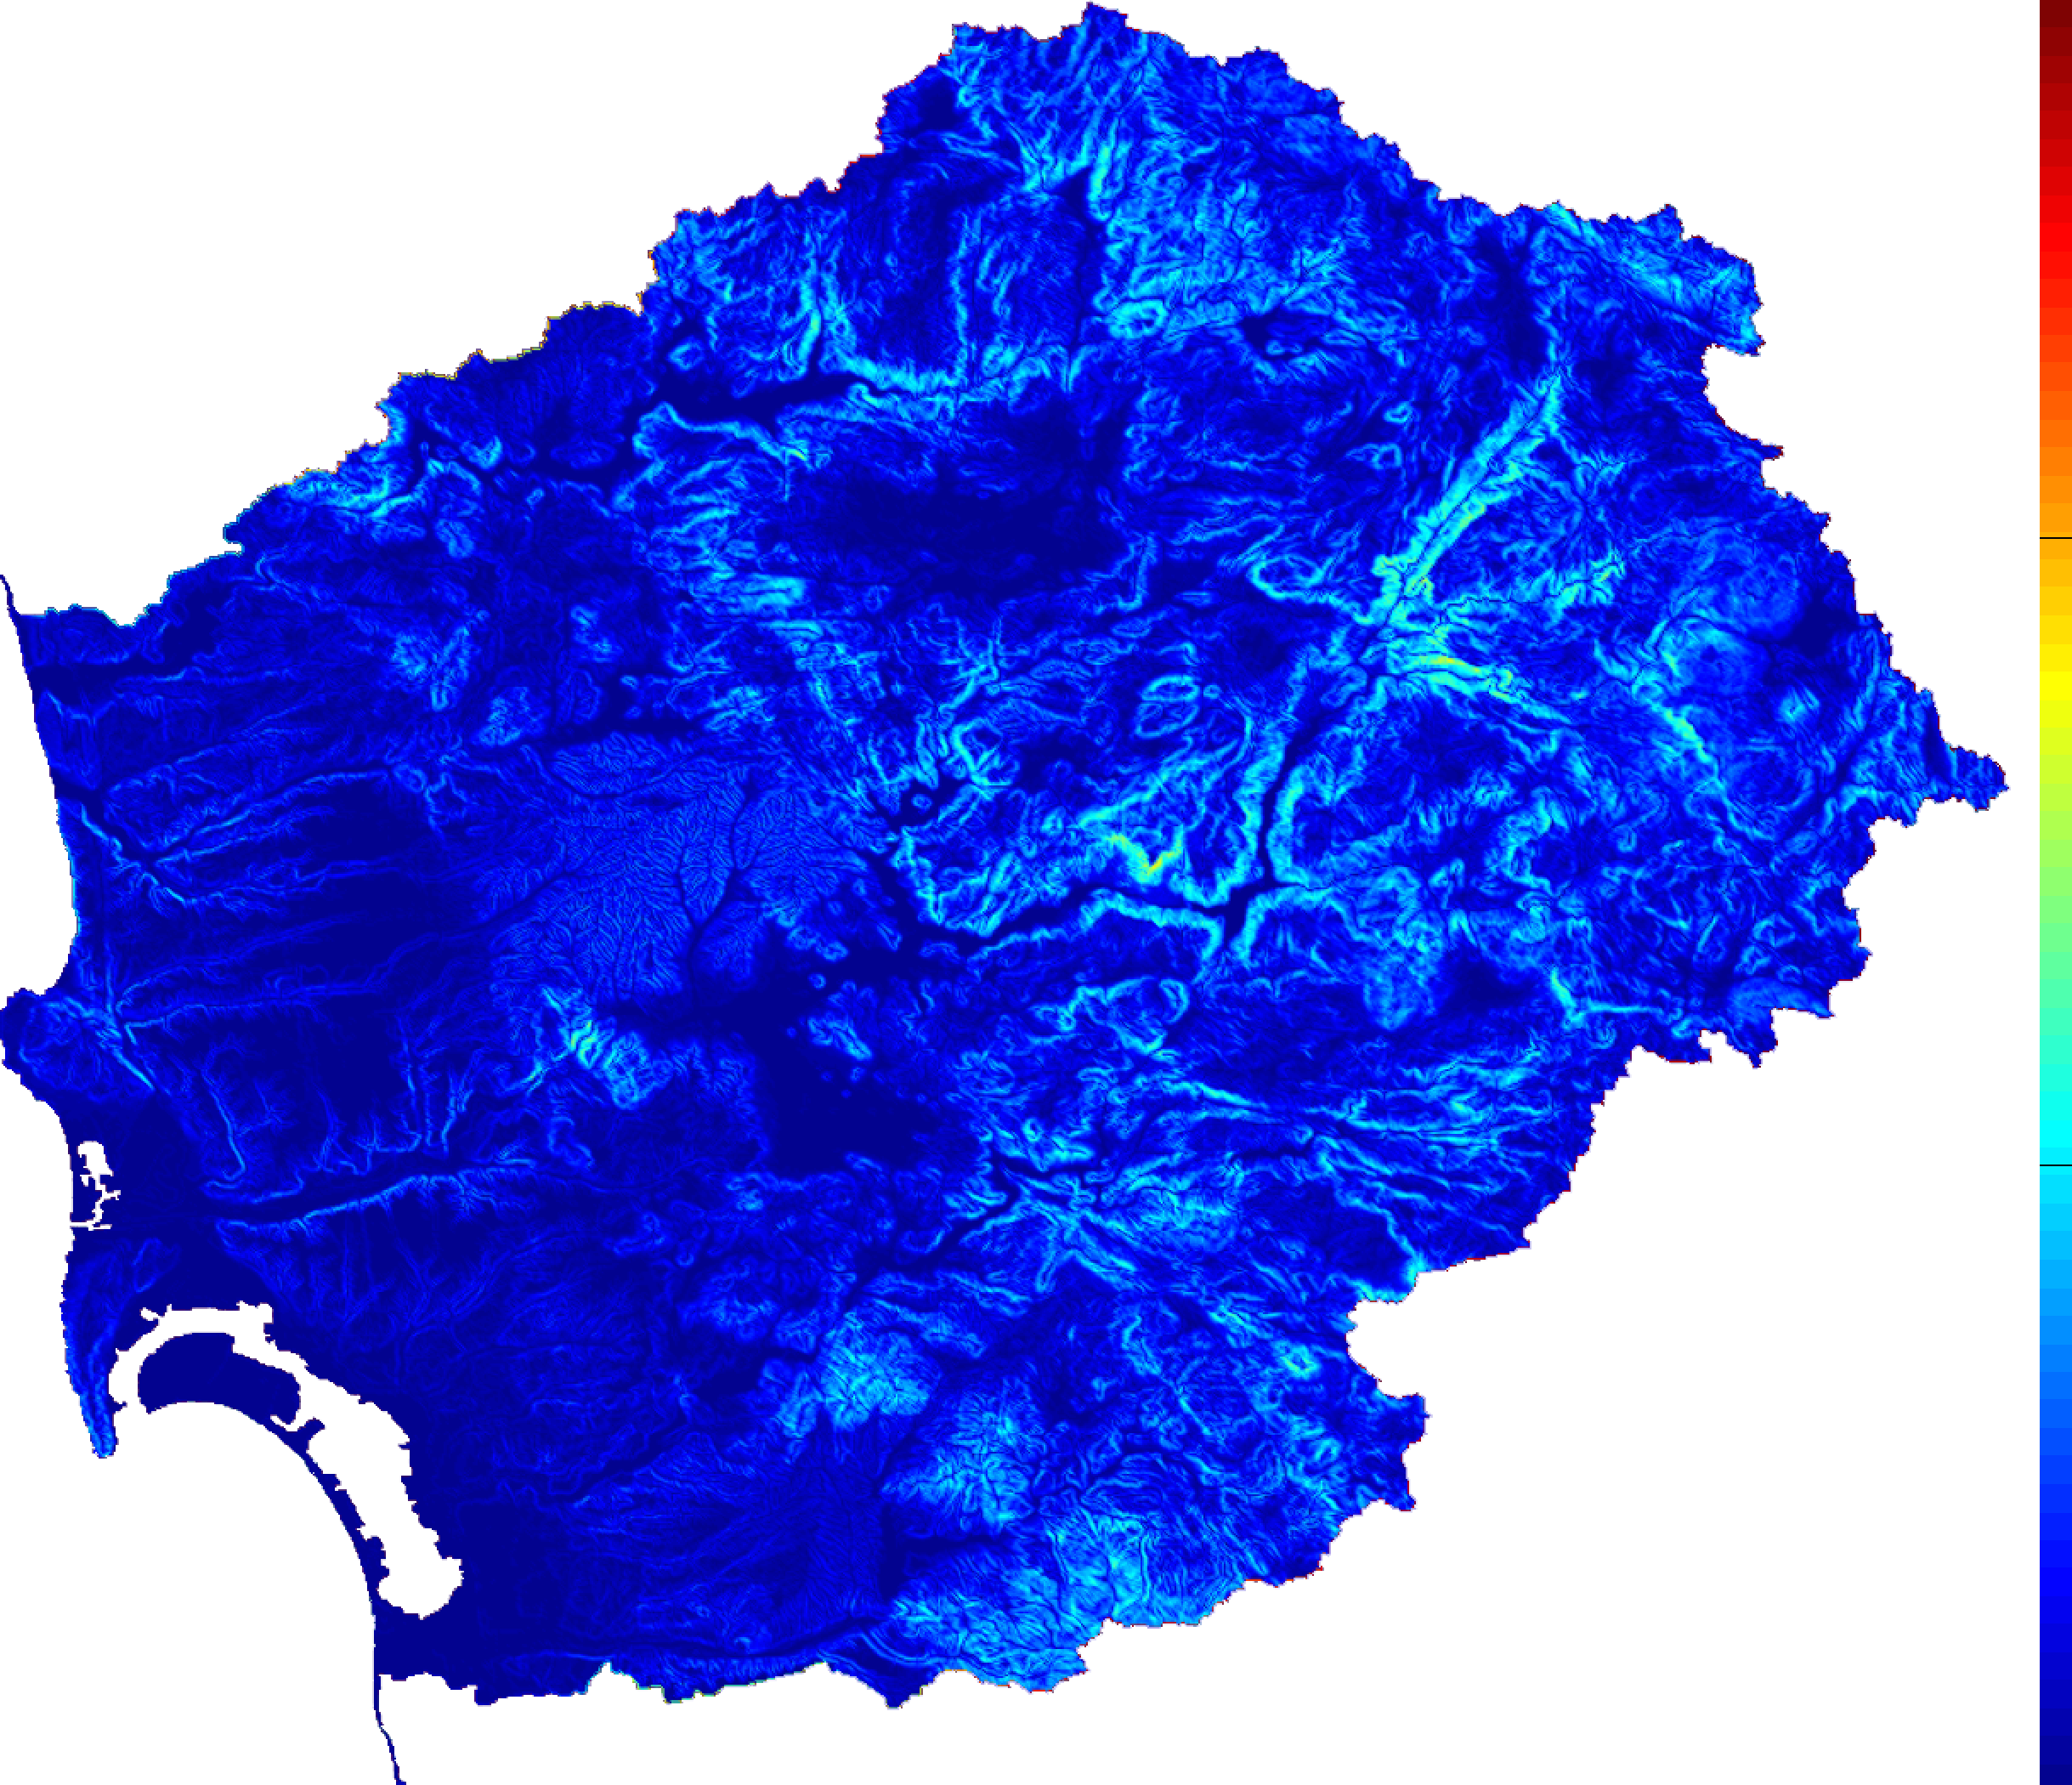
\includegraphics[width=5.5in]{figures/SanDiego_SlopeScore.png}   
            \caption{San Diego Region Slope Based Objective Scores (Blue:Low, Red:High)}
            \label{fig:SDslope}
            \end{center}
        \end{figure}
        
    \subsection{Proposed Corridor Solutions}
    
        \begin{figure}[!h]
            \begin{center}
            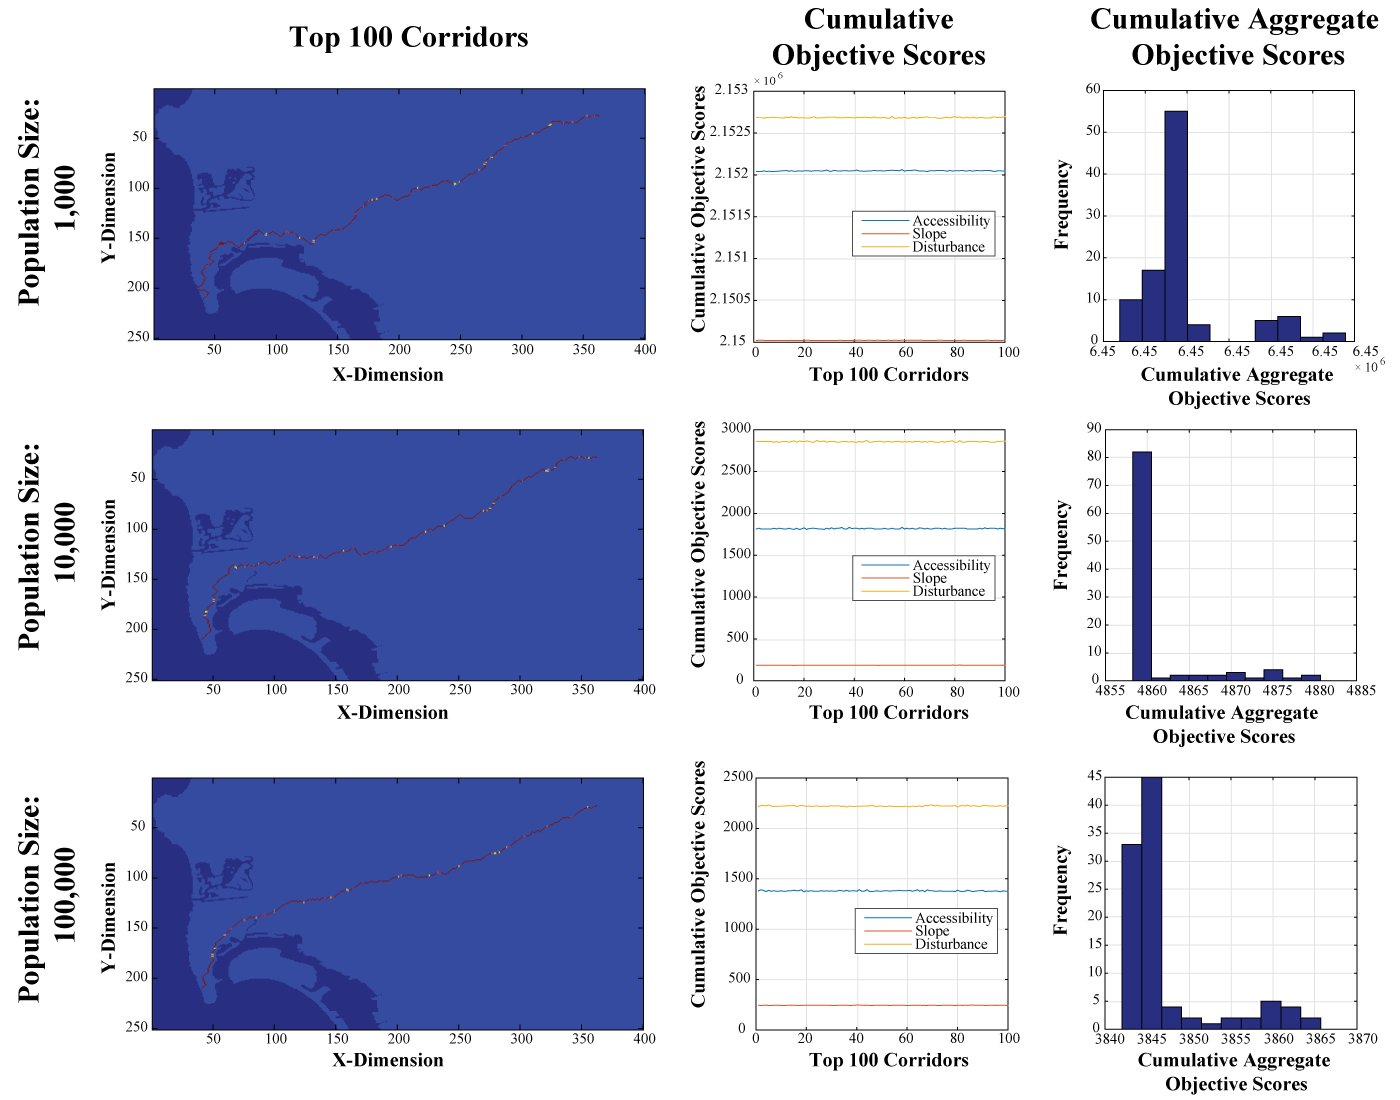
\includegraphics[width=6in]{figures/SanDiego_PathwayResults.png}   
            \caption{San Diego Region Corridor Analysis Results}
            \label{fig:SDresults}
            \end{center}
        \end{figure}

        \begin{figure}[!h]
            \begin{center}
            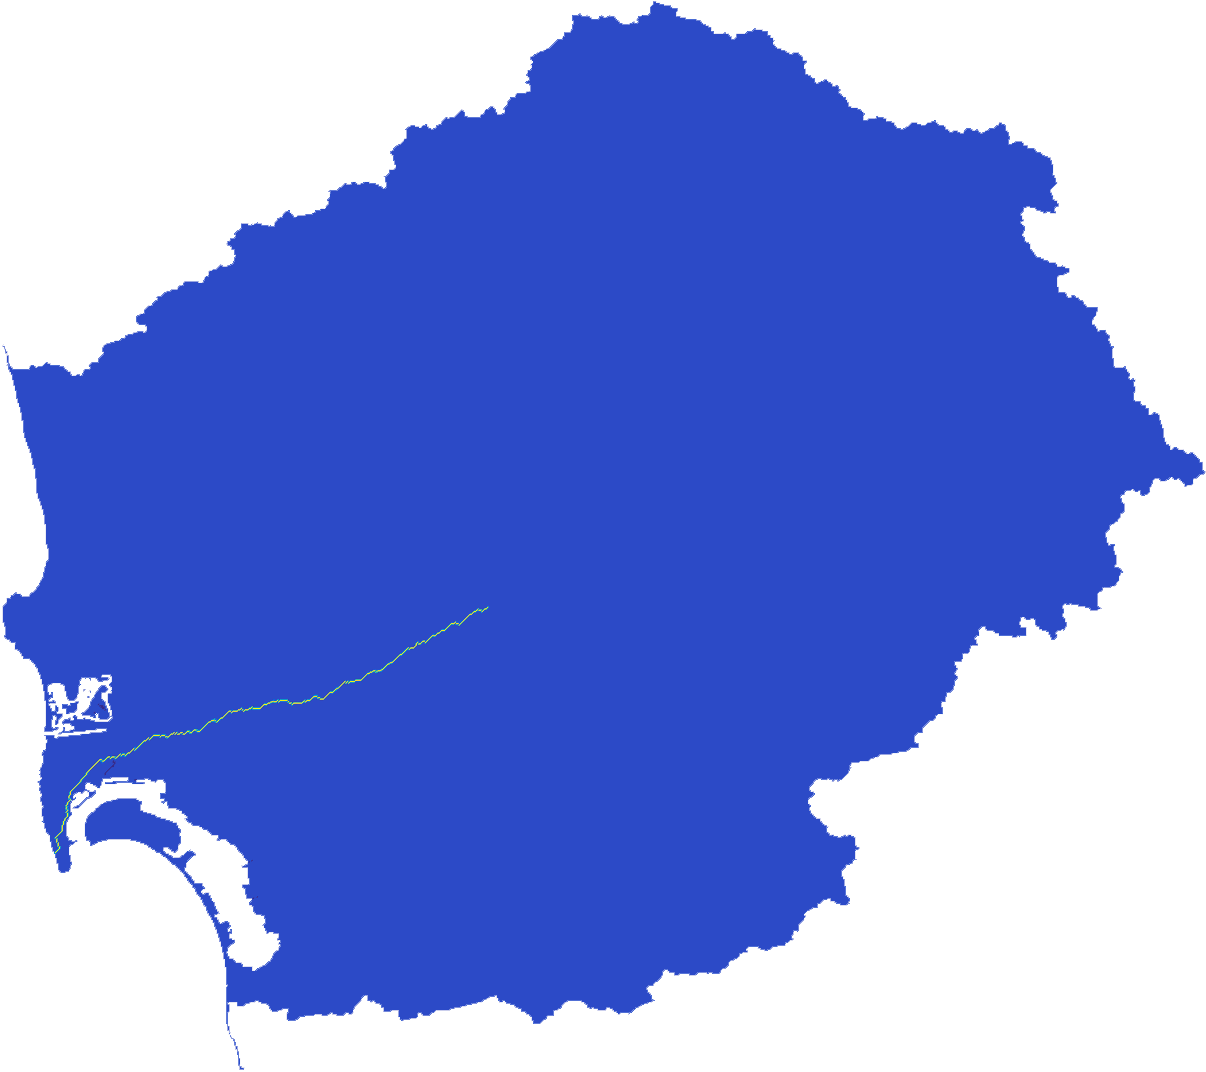
\includegraphics[width=5.5in]{figures/SanDiego_PathwayLarge.png}   
            \caption{San Diego Region Top 100 Corridors (Pop Size: 100,000) Basin Wide Overview}
            \label{fig:SDsolutionOverview}
            \end{center}
        \end{figure}
        
        \begin{figure}[!h]
            \begin{center}
            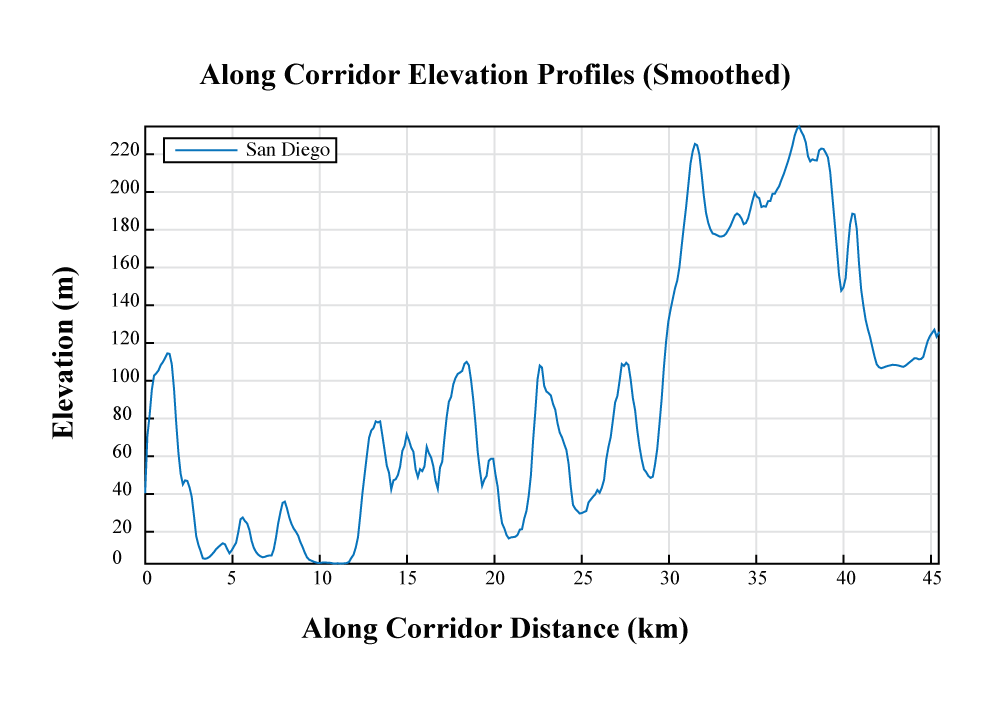
\includegraphics[width=5.5in]{figures/SanDiego_Elevation_Profile.png}   
            \caption{Santa Diego Region Proposed Corridor Elevation Profile}
            \label{fig:SDelevationProfile}
            \end{center}
        \end{figure}
    
    \subsection{Anticipated Distribution of Life Cycle Energy Usages and Net Water Savings}

\clearpage

\section{Santa Ana -- San Bernadino Region}

    \subsection{Regional Context}

    \begin{itemize}
      \setlength{\itemsep}{0cm}
      \setlength{\parskip}{0cm}
        \item HUC-8 Code: $18070203$
        \item Total Area: $5,375.9$ $km^2$
        \item Maximum Elevation: $3,461.3$ $m$
        \item Minimum Elevation: $-0.7$ $m$
        \item Mean Slope: $10.56$ $\%$
        \item Standard Deviation of Slope: $12.21$ $\%$
        \item Dominant Soil Composition: Hydrologic Soil Group - B: $10-20\%$ clay, $50-90\%$ sand, $35\%$ rock fragments
    \end{itemize}
    
        \begin{figure}[!h]
            \begin{center}
            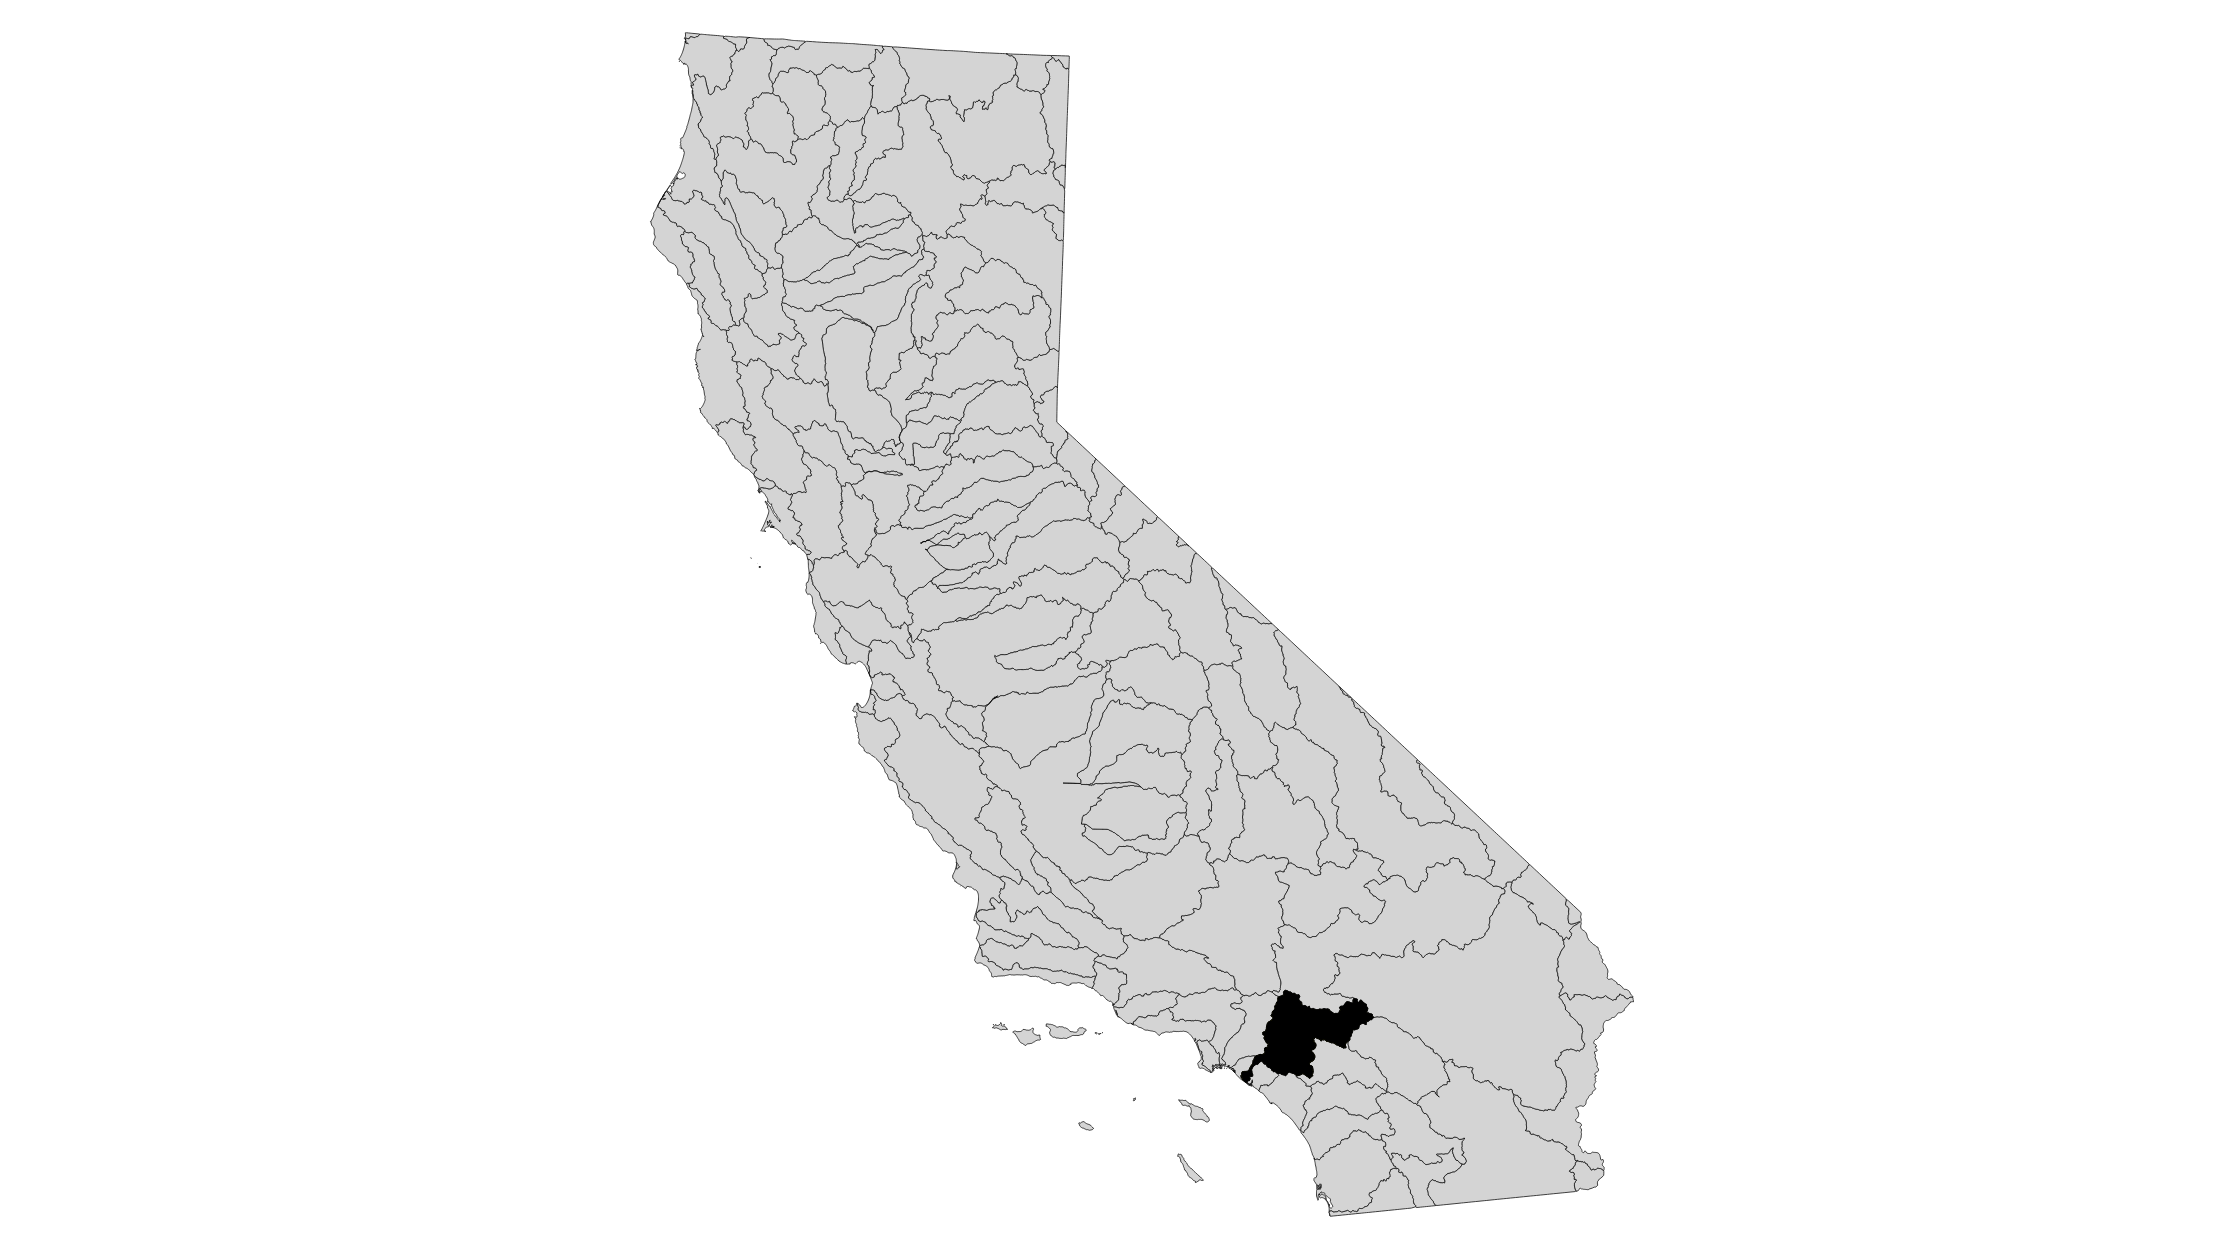
\includegraphics[width=5.5in]{figures/SanBernadino_Overview.png}   
            \caption{Santa Ana -- San Bernadino Region Overview (Filled in Black)}
            \label{fig:SASBoverview}
            \end{center}
        \end{figure}

    \subsection{Search Domain}
    
    \begin{itemize}
      \setlength{\itemsep}{0cm}
      \setlength{\parskip}{0cm}
        \item Grid Dimensions: $854$ $cells$ x $1463$ $cells$
        \item Grid Cell Resolution: $100$ $m$ x $100$ $m$ ($1$ $ha$)
        \item Feasible Grid Cells: $537,587$ $cells$
    \end{itemize}
    
        \begin{figure}[!h]
            \begin{center}
            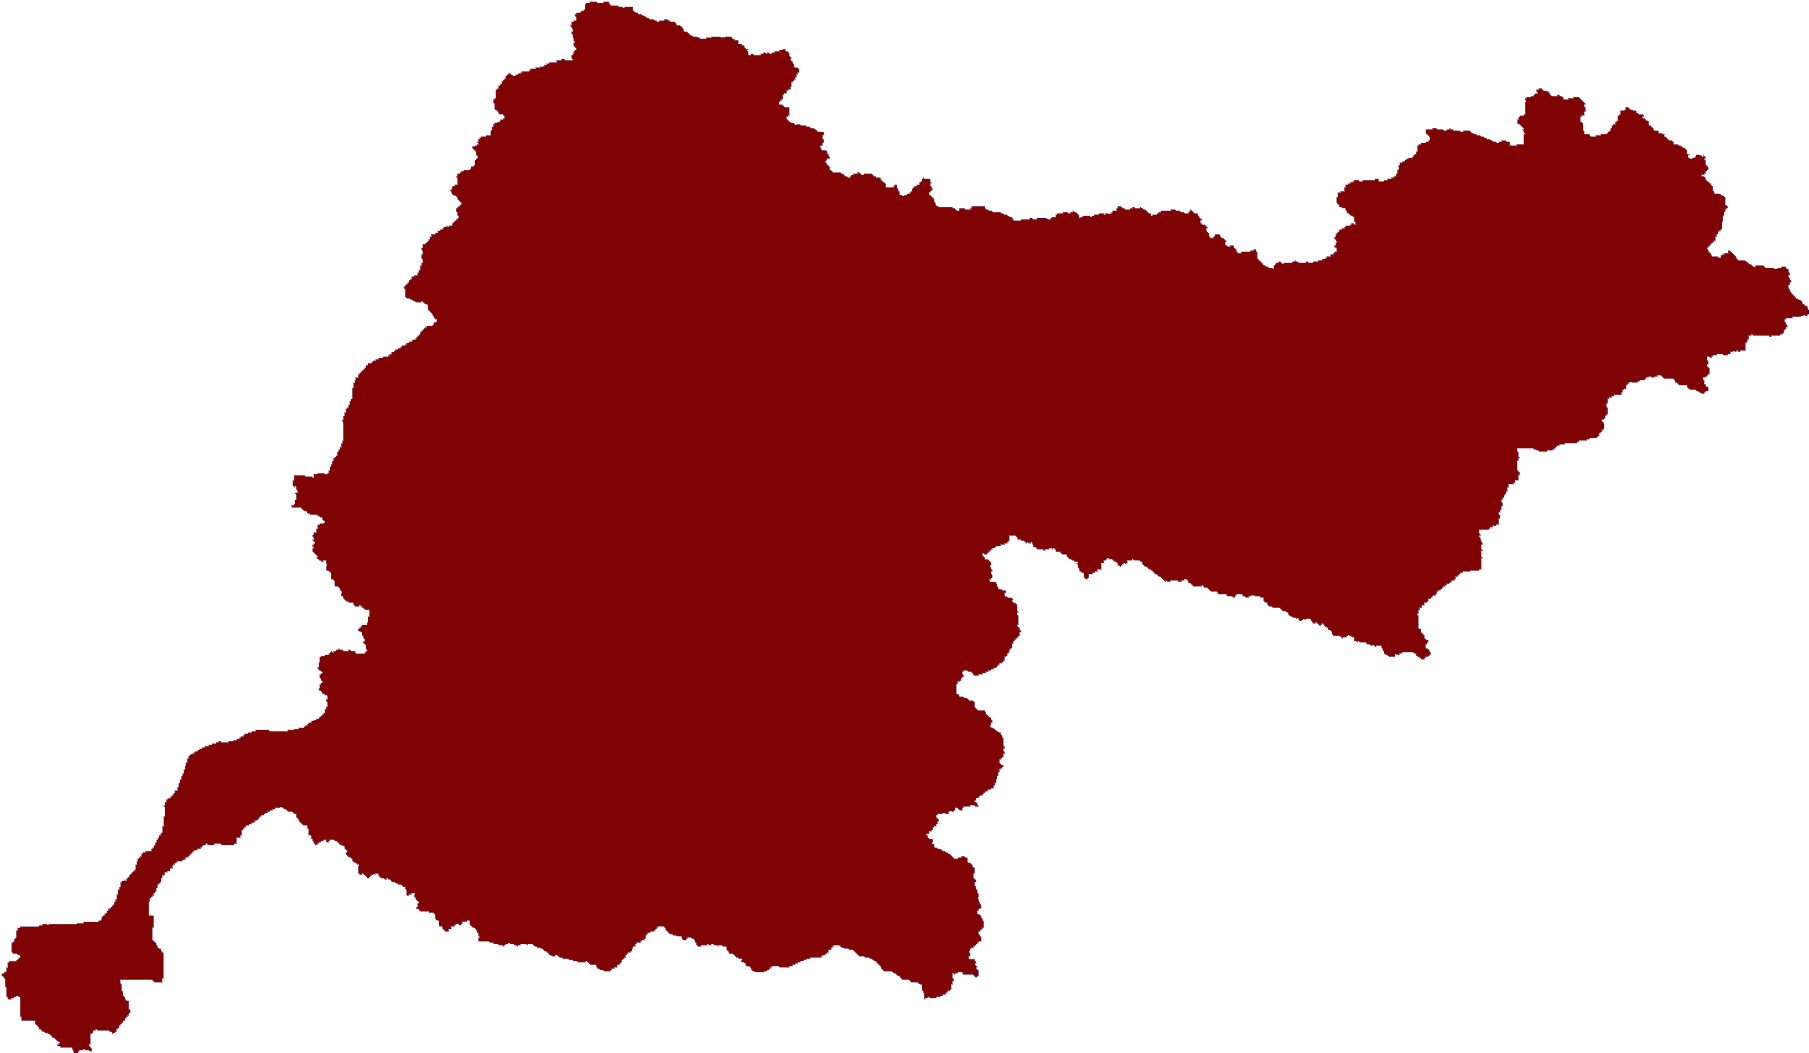
\includegraphics[width=5.5in]{figures/SanBernadino_SearchDomain.png}   
            \caption{Santa Ana -- San Bernadino Region Search Domain (Filled in Red)}
            \label{fig:SASBdomain}
            \end{center}
        \end{figure}
        
\subsection{Destination Search Inputs}
    
        \begin{figure}[!h]
            \begin{center}
            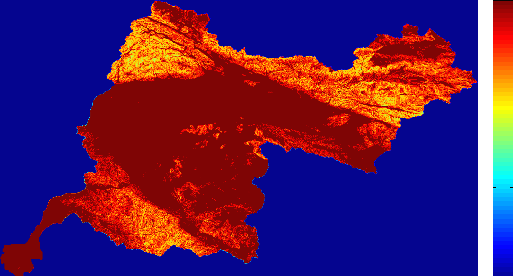
\includegraphics[width=5.5in]{figures/SanBernadino_Search_Slope.png}   
            \caption{Santa Ana -- San Bernadino Region Destination Search Inputs: Slope Score (Blue:Low, Red:High)}
            \label{fig:SASBdsinputs_slope}
            \end{center}
        \end{figure}
        
        \begin{figure}[!h]
            \begin{center}
            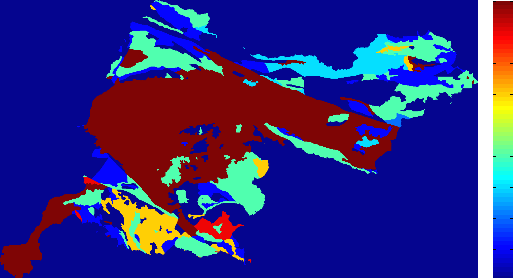
\includegraphics[width=5.5in]{figures/SanBernadino_Search_Geology.png}   
            \caption{Santa Ana -- San Bernadino Region Destination Search Inputs: Geology Score (Blue:Low, Red:High)}
            \label{fig:SASBdsinputs_geology}
            \end{center}
        \end{figure}
    
        \begin{figure}[!h]
            \begin{center}
            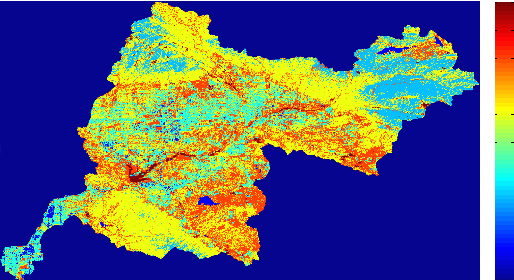
\includegraphics[width=5.5in]{figures/SanBernadino_Search_Landuse.png}   
            \caption{Santa Ana -- San Bernadino Region Destination Search Inputs: Landuse Score (Blue:Low, Red:High)}
            \label{fig:SASBdsinputs_landuse}
            \end{center}
        \end{figure}
    
    \subsection{Destination Search Outputs}
    
        \begin{figure}[!h]
            \begin{center}
            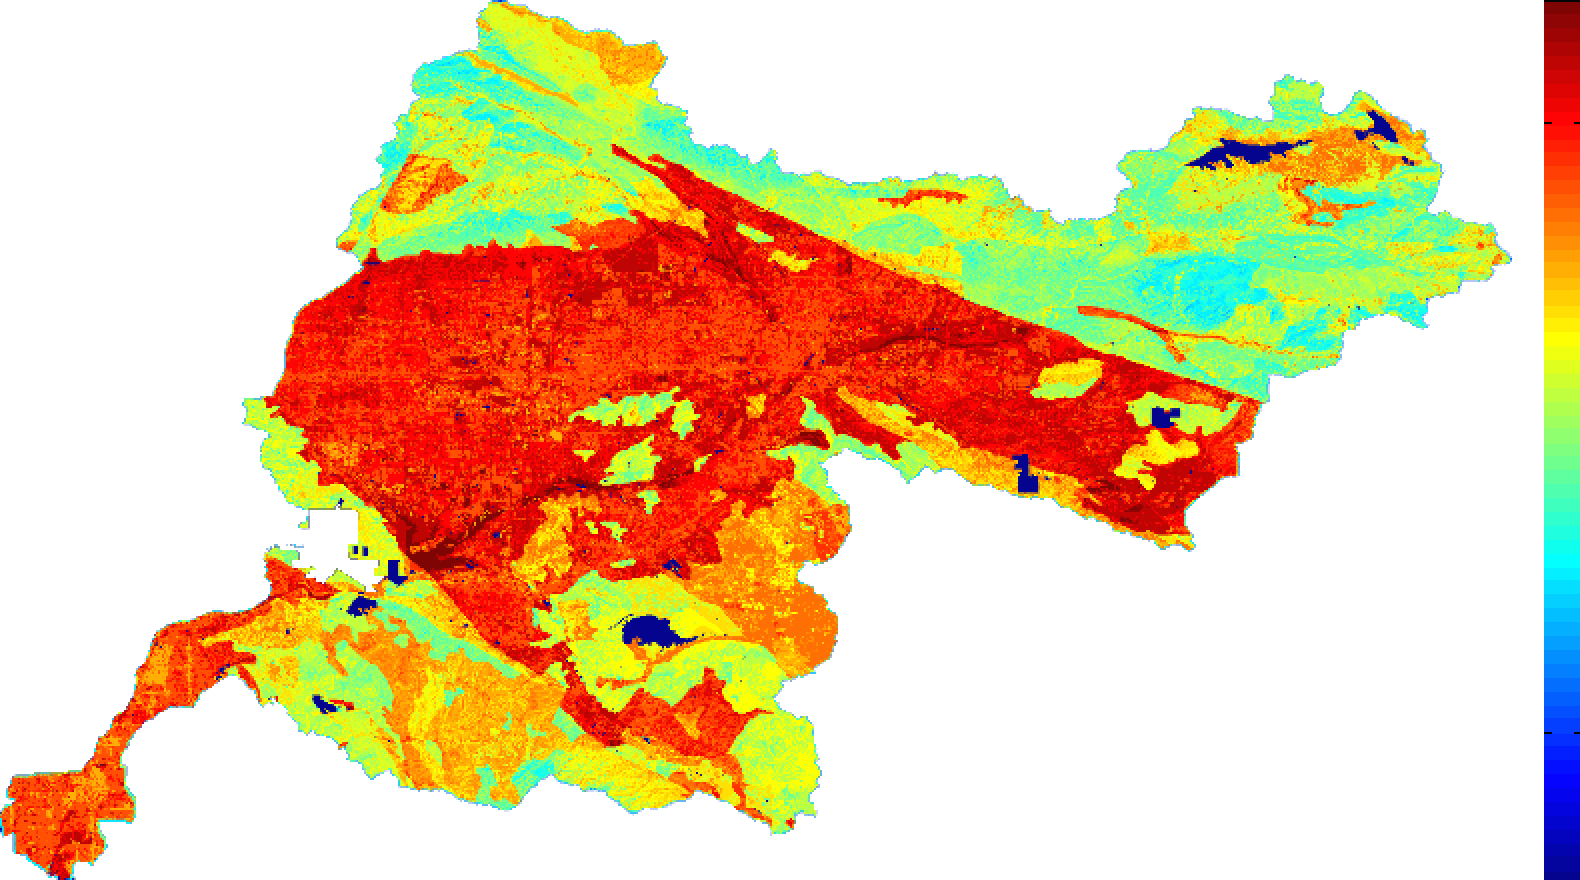
\includegraphics[width=5.5in]{figures/SanBernadino_Search_Composite.png}   
            \caption{Santa Ana -- San Bernadino Region Destination Search Outputs: Composite Scores (Blue:Low, Red:High)}
            \label{fig:SASBdsoutputs_comp}
            \end{center}
        \end{figure}
        
        \begin{figure}[!h]
            \begin{center}
            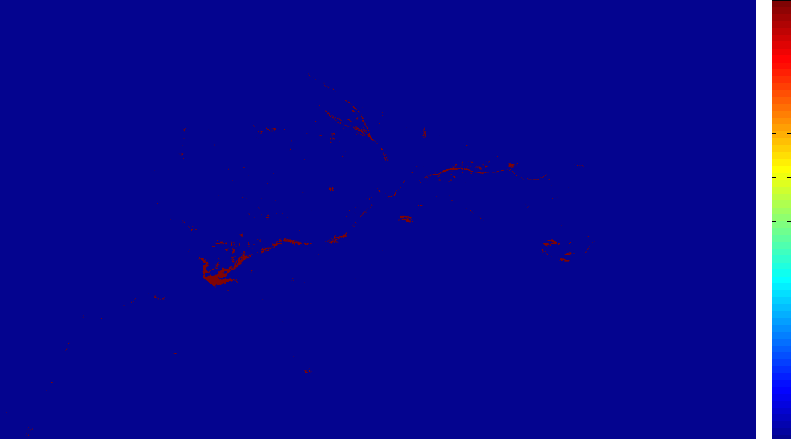
\includegraphics[width=5.5in]{figures/SanBernadino_Search_Output.png}   
            \caption{Santa Ana -- San Bernadino Region Destination Search Outputs: Candidate Regions}
            \label{fig:SASBdsoutputs_cand}
            \end{center}
        \end{figure}

    \subsection{Proposed Corridor Endpoints}
    
    \begin{itemize}
      \setlength{\itemsep}{0cm}
      \setlength{\parskip}{0cm}
        \item Start Location: $(840,48)$
        \item End Destination: $(528,430)$
        \item Shortest Euclidean Path Distance: $49,322$ $m$ ($49$ $km$)
    \end{itemize}
    
        \begin{figure}[!h]
            \begin{center}
            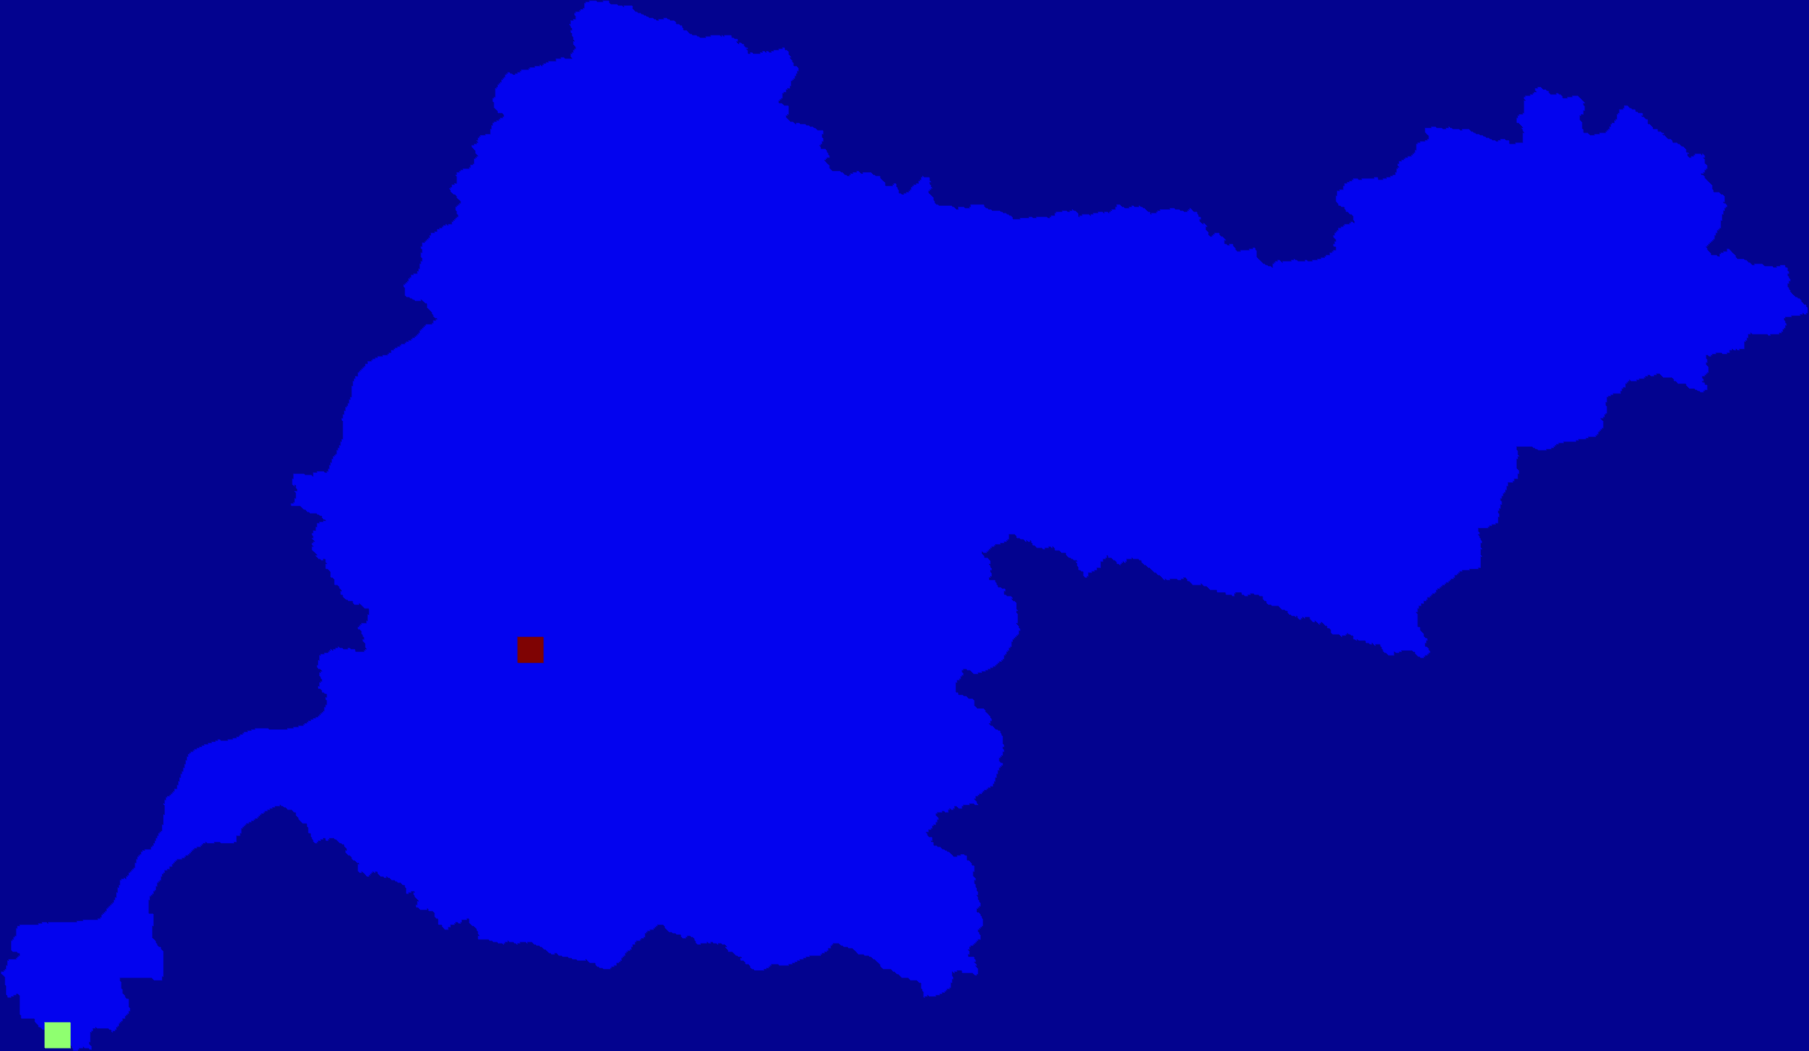
\includegraphics[width=5.5in]{figures/SanBernadino_Endpoints.png}   
            \caption{Santa Ana -- San Bernadino Region Proposed Corridor Endpoints}
            \label{fig:SASBendpoints}
            \end{center}
        \end{figure}
    
    \subsection{Proposed Objective Layers}

        \begin{figure}[!h]
            \begin{center}
            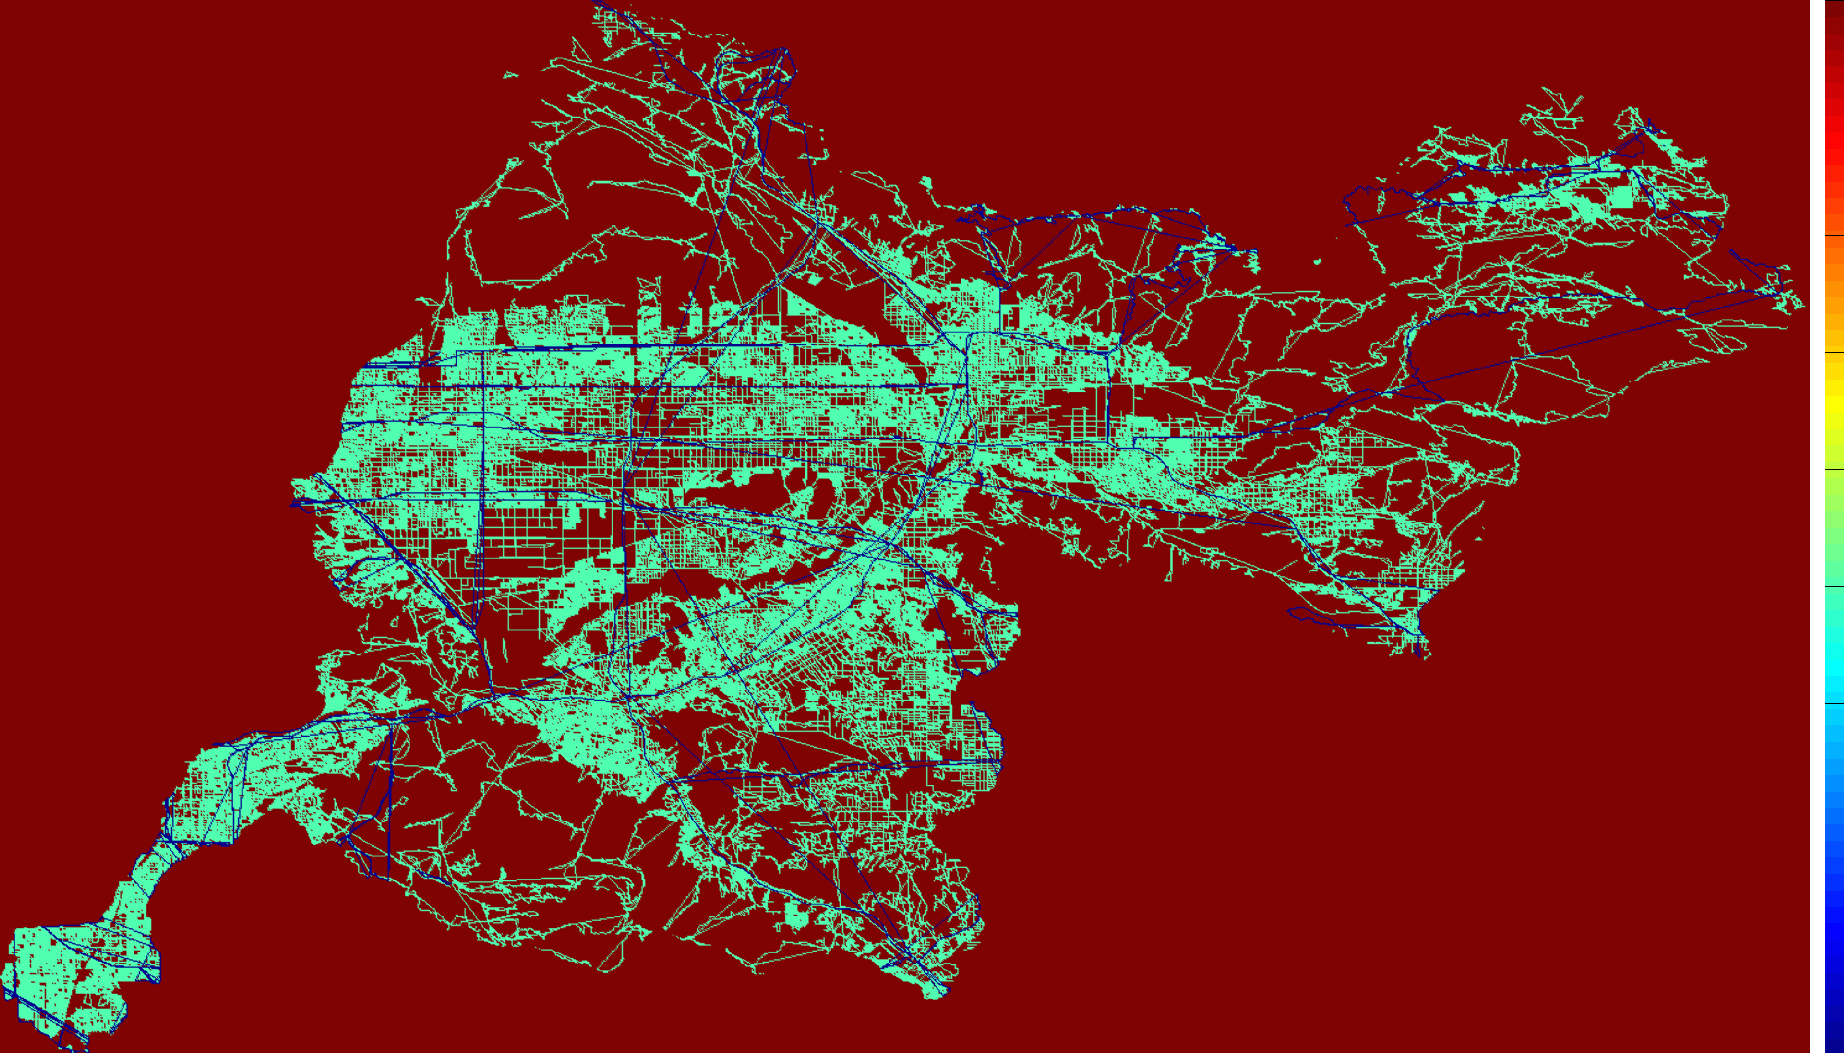
\includegraphics[width=5.5in]{figures/SanBernadino_AccessibilityScore.png}   
            \caption{Santa Ana -- San Bernadino Region Accessibility Based Objective Scores (Blue:Low, Red:High)}
            \label{fig:SASBaccessibilty}
            \end{center}
        \end{figure}

        \begin{figure}[!h]
            \begin{center}
            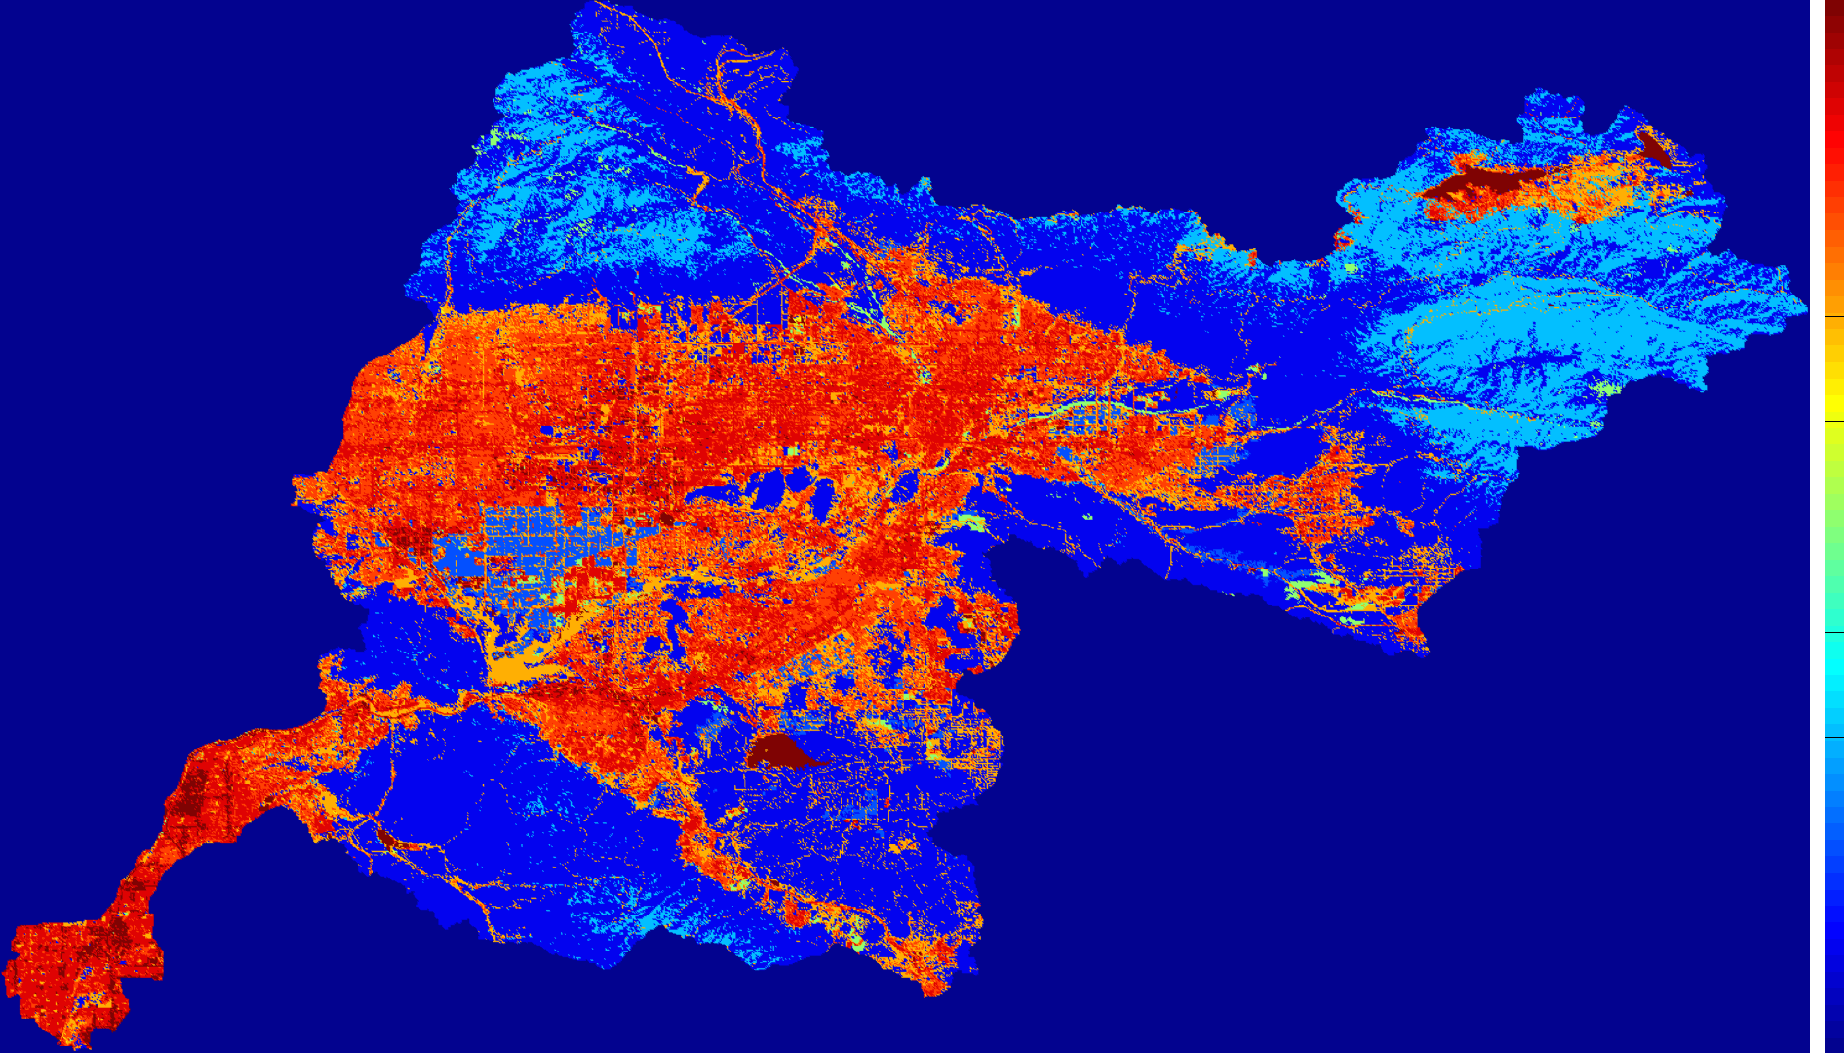
\includegraphics[width=5.5in]{figures/SanBernadino_DisturbanceScore.png}   
            \caption{Santa Ana -- San Bernadino Region Land Use Disturbance Based Objective Scores (Blue:Low, Red:High)}
            \label{fig:SASBdisturbance}
            \end{center}
        \end{figure}
        
        \begin{figure}[!h]
            \begin{center}
            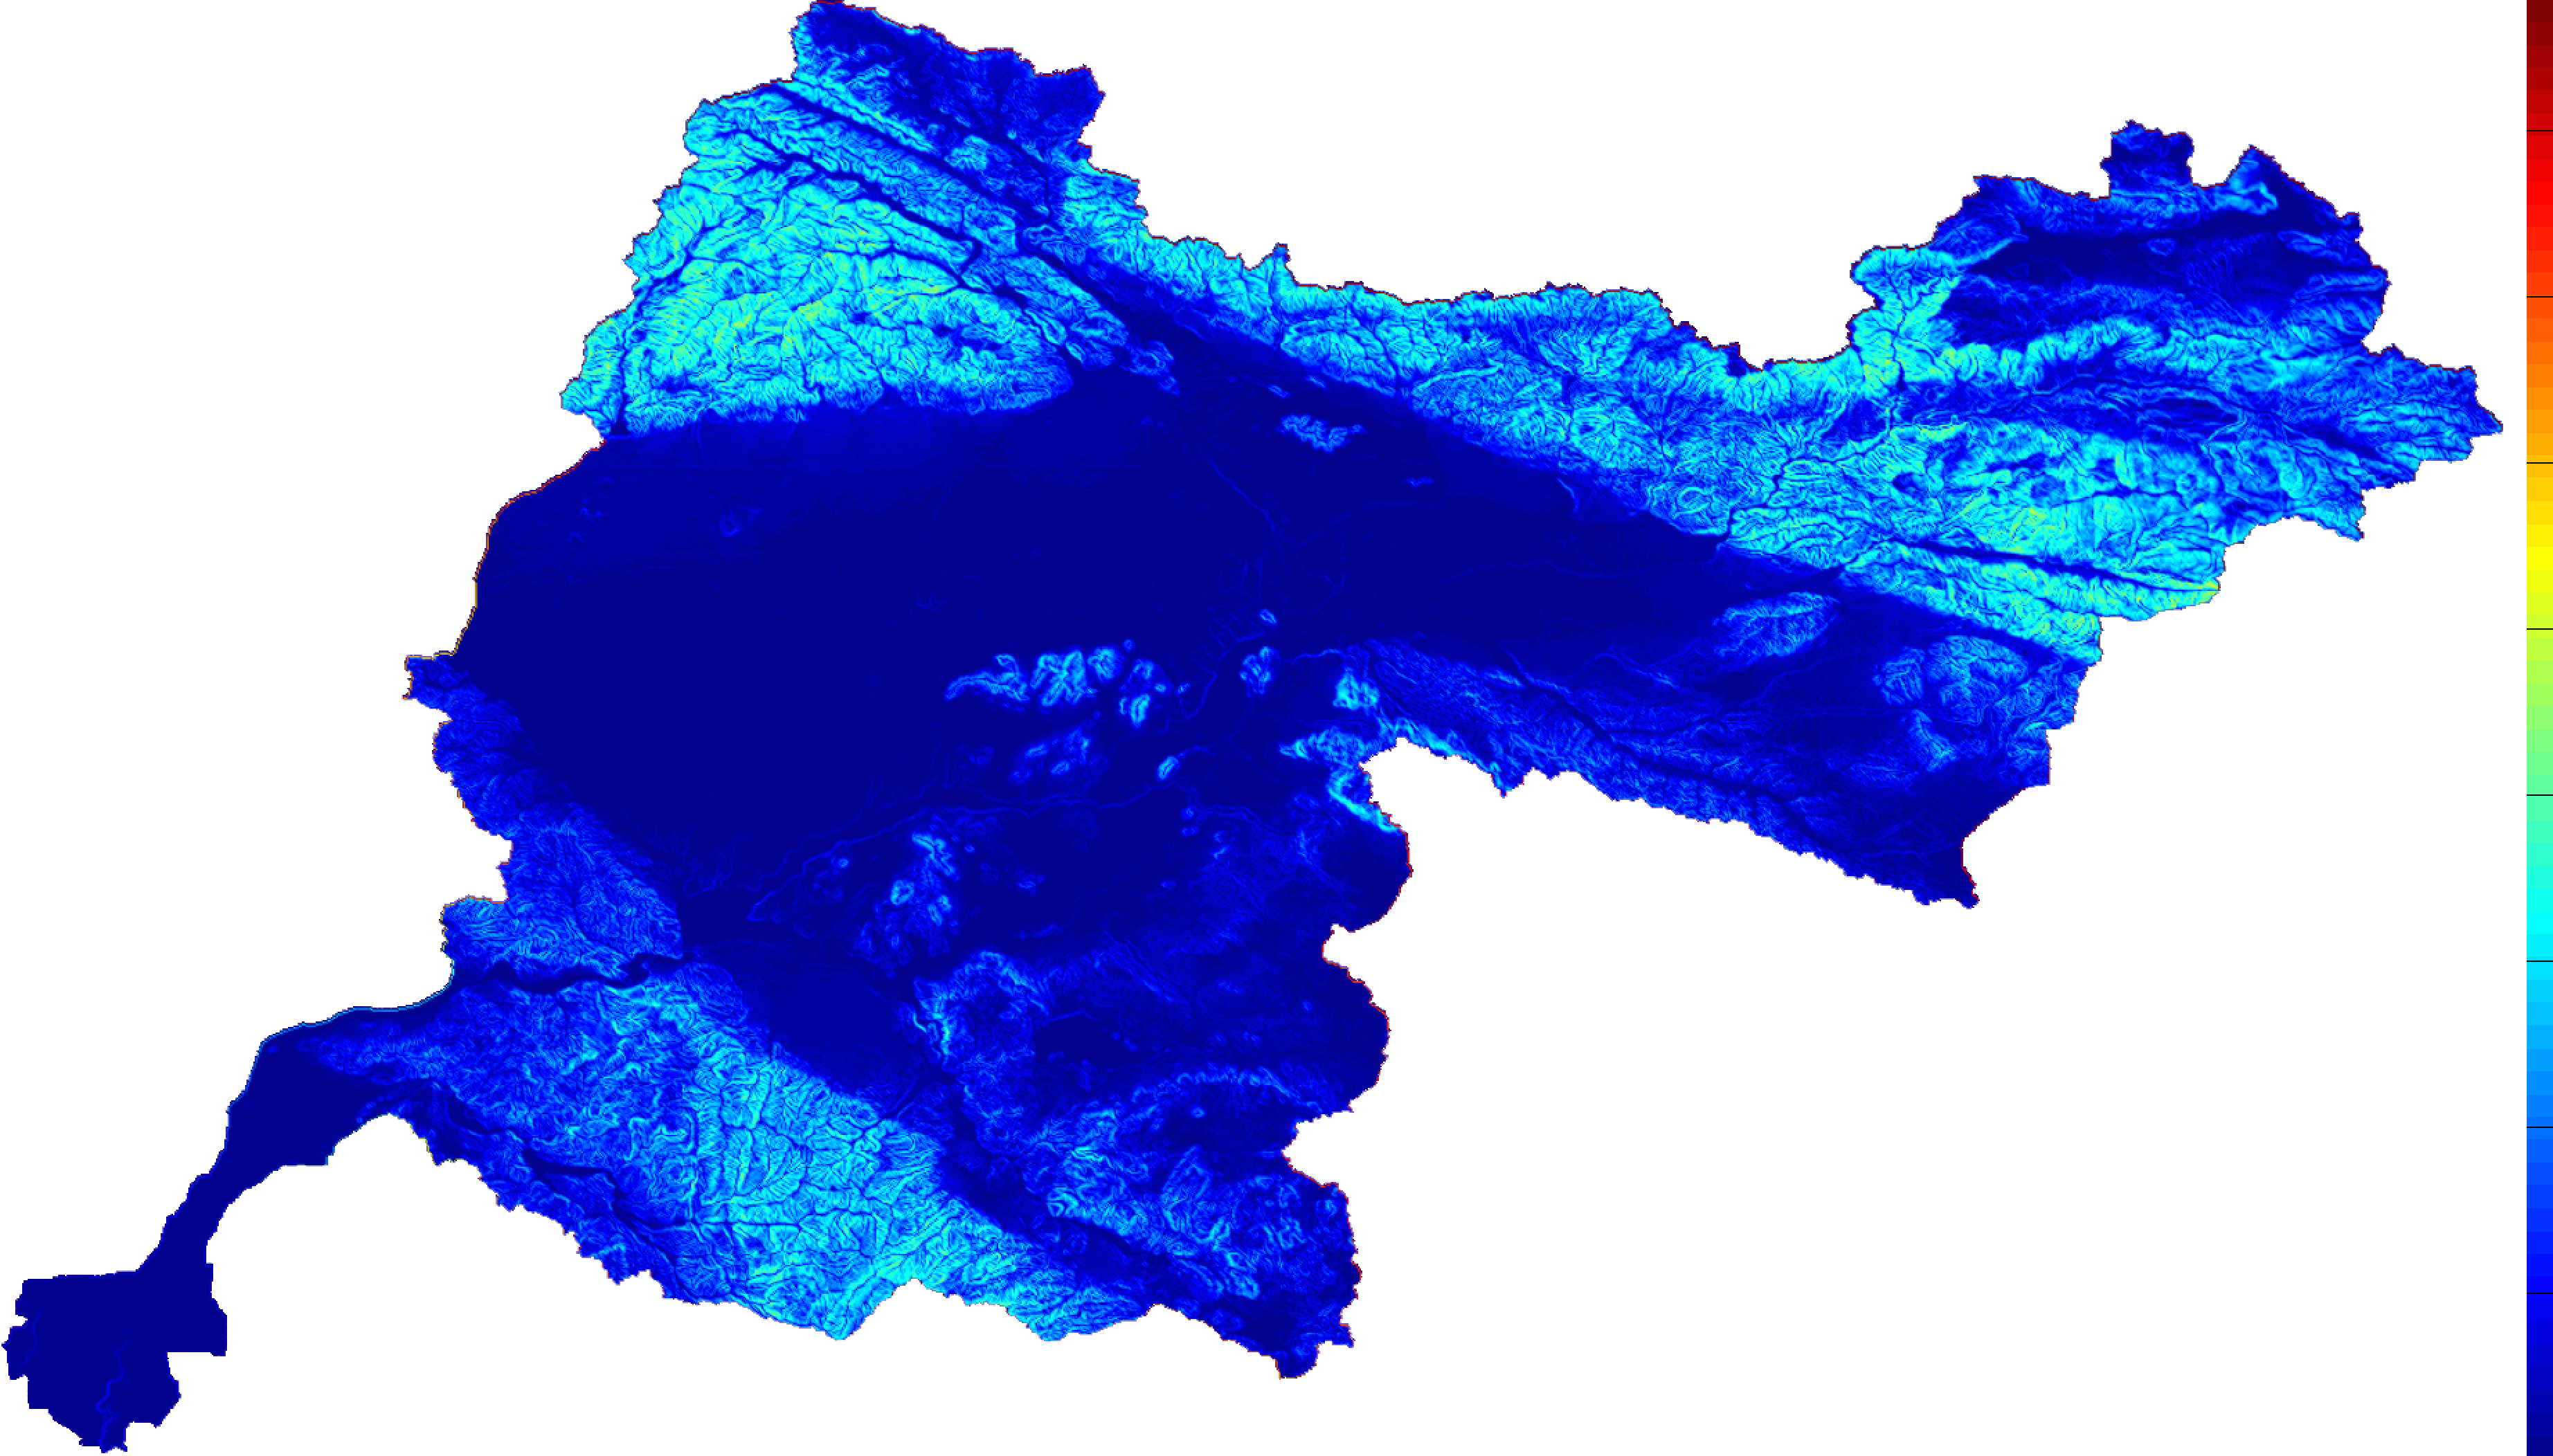
\includegraphics[width=5.5in]{figures/SanBernadino_SlopeScore.png}   
            \caption{Santa Ana -- San Bernadino Region Slope Based Objective Scores (Blue:Low, Red:High)}
            \label{fig:SASBslope}
            \end{center}
        \end{figure}
        
    \subsection{Proposed Corridor Solutions}
    
        \begin{figure}[!h]
            \begin{center}
            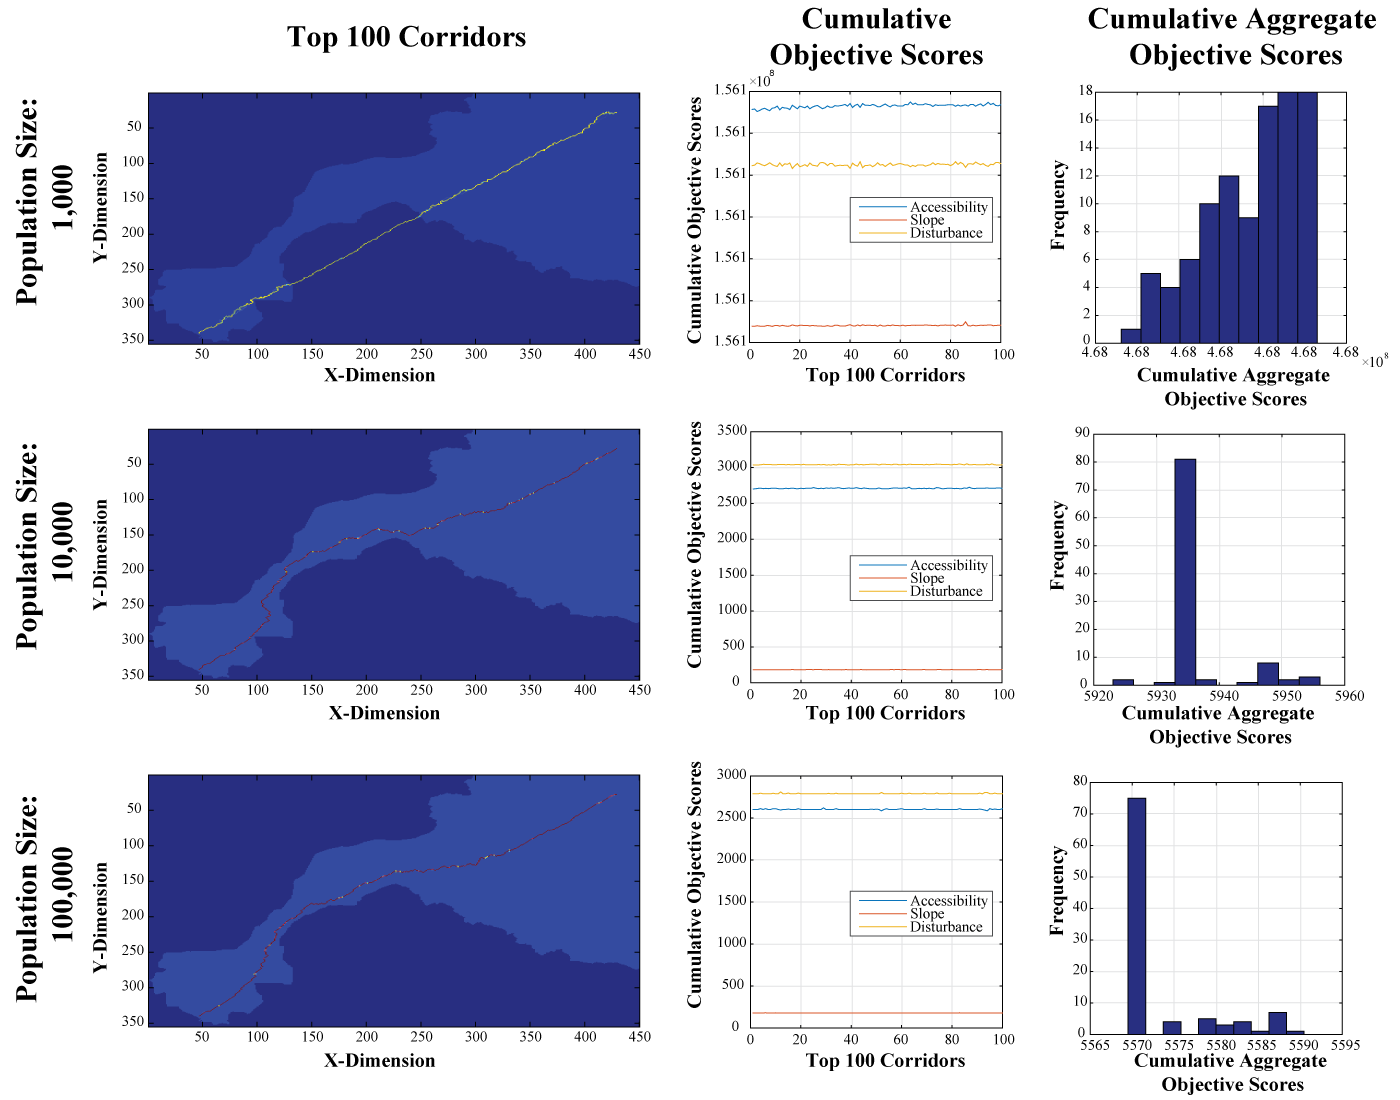
\includegraphics[width=6in]{figures/SanBernadino_PathwayResults.png}   
            \caption{Santa Ana -- San Bernadino Region Corridor Analysis Results}
            \label{fig:SASBresults}
            \end{center}
        \end{figure}

        \begin{figure}[!h]
            \begin{center}
            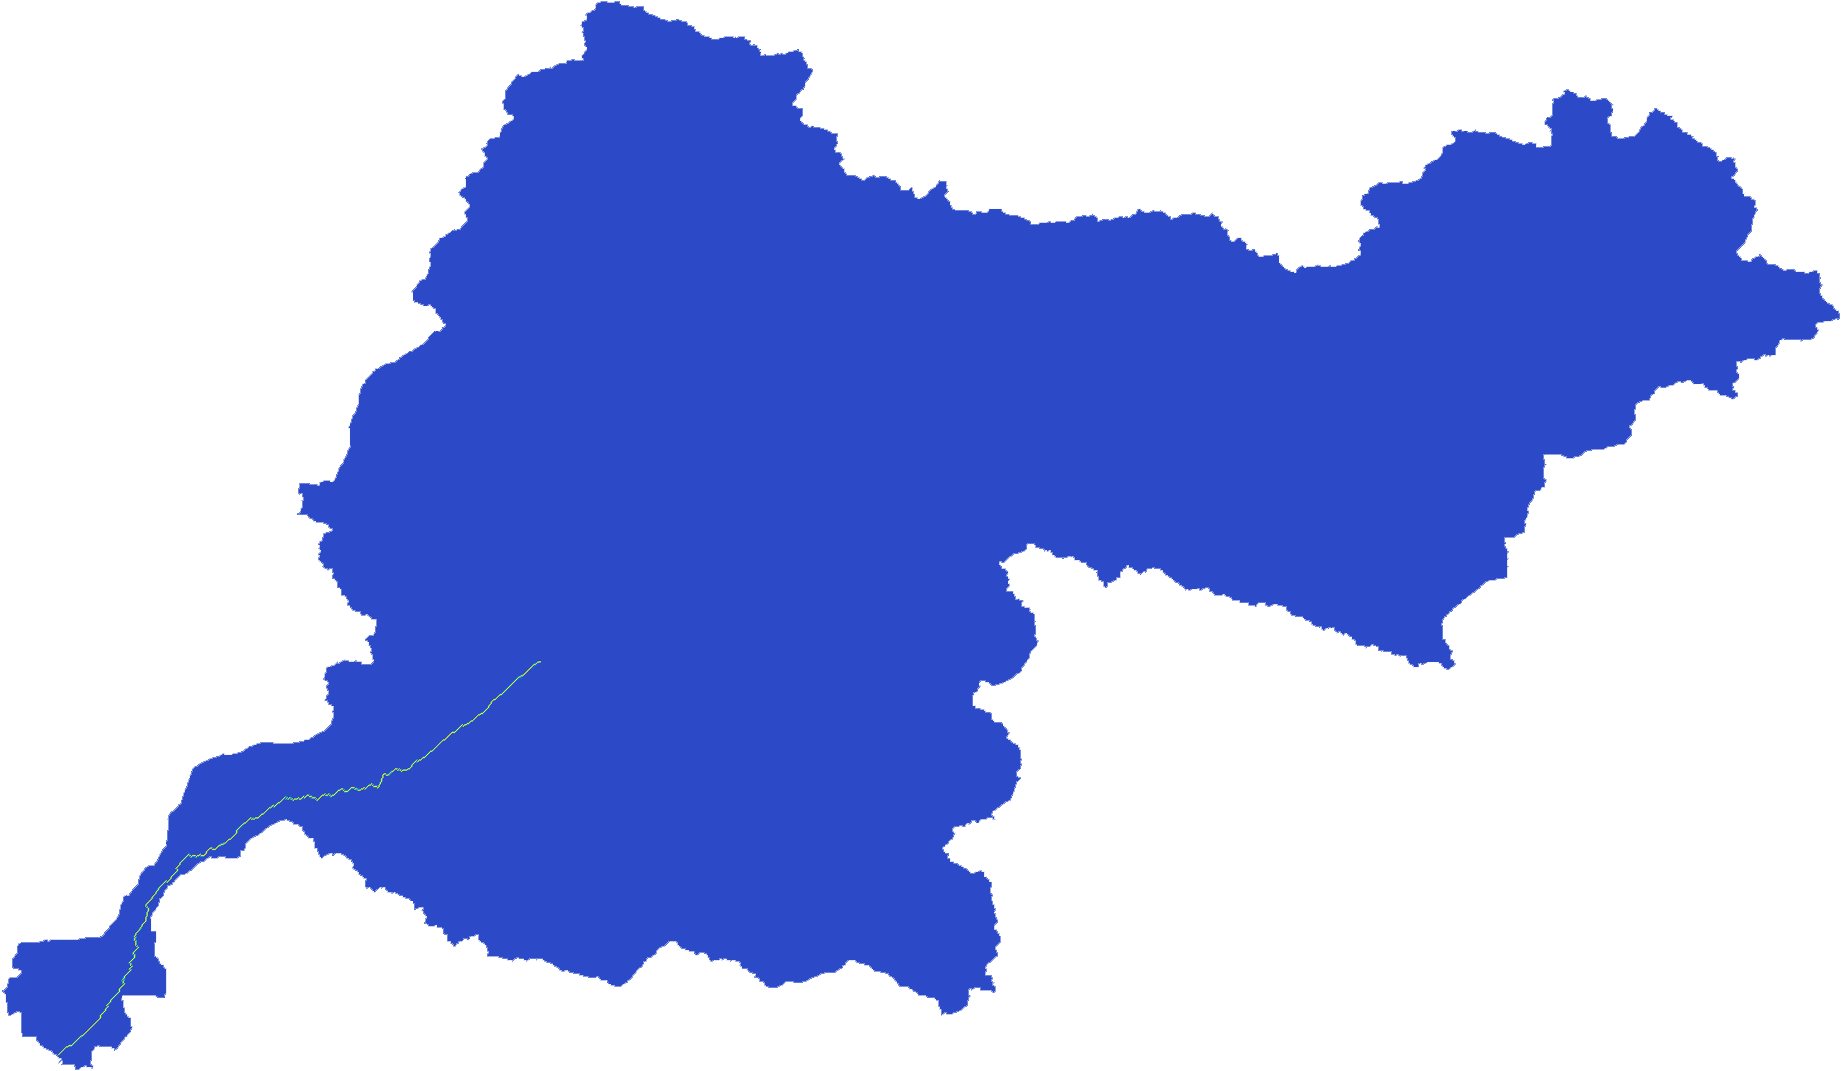
\includegraphics[width=5.5in]{figures/SanBernadino_PathwayLarge.png}   
            \caption{Santa Ana -- San Bernadino Region Top 100 Corridors (Pop Size: 100,000) Basin Wide Overview}
            \label{fig:SASBsolutionOverview}
            \end{center}
        \end{figure}
        
        \begin{figure}[!h]
            \begin{center}
            \includegraphics[width=5.5in]{figures/SanBernadino_Elevation_Profile.png}   
            \caption{San Bernadino Region Proposed Corridor Elevation Profile}
            \label{fig:SASBelevationProfile}
            \end{center}
        \end{figure}
    
    \subsection{Anticipated Distribution of Life Cycle Energy Usages and Net Water Savings}

\clearpage

\section{Fresno -- Tulare Region}

    \subsection{Regional Context}

    \begin{itemize}
      \setlength{\itemsep}{0cm}
      \setlength{\parskip}{0cm}
        \item HUC-8 Code: $18030009$
        \item Total Area: $6,943.6$ $km^2$
        \item Maximum Elevation: $1,536.6$ $m$
        \item Minimum Elevation: $0$ $m$
        \item Mean Slope: $2.16$ $\%$
        \item Standard Deviation of Slope: $6.24$ $\%$
        \item Dominant Soil Composition: Hydrologic Soil Group - B: $10-20\%$ clay, $50-90\%$ sand, $35\%$ rock fragments
    \end{itemize}

        \begin{figure}[!h]
            \begin{center}
            \includegraphics[width=5.5in]{figures/Fresno_Overview.png}   
            \caption{Fresno -- Tulare Region Overview (Filled in Black)}
            \label{fig:Foverview}
            \end{center}
        \end{figure}

    \subsection{Search Domain}
    
    \begin{itemize}
      \setlength{\itemsep}{0cm}
      \setlength{\parskip}{0cm}
        \item Grid Dimensions: $1018$ $cells$ x $1459$ $cells$
        \item Grid Cell Resolution: $100$ $m$ x $100$ $m$ ($1$ $ha$)
        \item Feasible Grid Cells: $694,365$ $cells$
    \end{itemize}
    
        \begin{figure}[!h]
            \begin{center}
            \includegraphics[width=5.5in]{figures/Fresno_SearchDomain.png}   
            \caption{Fresno -- Tulare Region Search Domain (Filled in Red)}
            \label{fig:Fdomain}
            \end{center}
        \end{figure}
        
    \subsection{Destination Search Inputs}
    
        \begin{figure}[!h]
            \begin{center}
            \includegraphics[width=5.5in]{figures/Fresno_Search_Slope.png}   
            \caption{Fresno -- Tulare Region Destination Search Inputs: Slope Score (Blue:Low, Red:High)}
            \label{fig:Fdsinputs_slope}
            \end{center}
        \end{figure}
        
        \begin{figure}[!h]
            \begin{center}
            \includegraphics[width=5.5in]{figures/Fresno_Search_Geology.png}   
            \caption{Fresno -- Tulare Region Destination Search Inputs: Geology Score (Blue:Low, Red:High)}
            \label{fig:Fdsinputs_geology}
            \end{center}
        \end{figure}
    
        \begin{figure}[!h]
            \begin{center}
            \includegraphics[width=5.5in]{figures/Fresno_Search_Landuse.png}   
            \caption{Fresno -- Tulare Region Destination Search Inputs: Landuse Score (Blue:Low, Red:High)}
            \label{fig:Fdsinputs_landuse}
            \end{center}
        \end{figure}
    
    \subsection{Destination Search Outputs}
    
        \begin{figure}[!h]
            \begin{center}
            \includegraphics[width=5.5in]{figures/Fresno_Search_Composite.png}   
            \caption{Fresno -- Tulare Region Destination Search Outputs: Composite Scores (Blue:Low, Red:High)}
            \label{fig:Fdsoutputs_comp}
            \end{center}
        \end{figure}
        
        \begin{figure}[!h]
            \begin{center}
            \includegraphics[width=5.5in]{figures/Fresno_Search_Output.png}   
            \caption{Fresno -- Tulare Region Destination Search Outputs: Candidate Regions}
            \label{fig:Fdsoutputs_cand}
            \end{center}
        \end{figure}

    \subsection{Proposed Corridor Endpoints}
    
    \begin{itemize}
      \setlength{\itemsep}{0cm}
      \setlength{\parskip}{0cm}
        \item Start Location: $(435,1037)$
        \item End Destination: $(421,387)$
        \item Shortest Euclidean Path Distance: $65,015$ $m$ ($65$ $km$)
    \end{itemize}
    
        \begin{figure}[!h]
            \begin{center}
            \includegraphics[width=5.5in]{figures/Fresno_Endpoints.png}   
            \caption{Fresno -- Tulare Region Proposed Corridor Endpoints}
            \label{fig:Fendpoints}
            \end{center}
        \end{figure}

    \subsection{Proposed Objective Layers}
    
        \begin{figure}[!h]
            \begin{center}
            \includegraphics[width=5.5in]{figures/Fresno_AccessibilityScore.png}   
            \caption{Fresno -- Tulare Region Accessibility Based Objective Scores (Blue:Low, Red:High)}
            \label{fig:Faccessibilty}
            \end{center}
        \end{figure}

        \begin{figure}[!h]
            \begin{center}
            \includegraphics[width=5.5in]{figures/Fresno_DisturbanceScore.png}   
            \caption{Fresno -- Tulare Region Land Use Disturbance Based Objective Scores (Blue:Low, Red:High)}
            \label{fig:Fdisturbance}
            \end{center}
        \end{figure}
        
        \begin{figure}[!h]
            \begin{center}
            \includegraphics[width=5.5in]{figures/Fresno_SlopeScore.png}   
            \caption{Fresno -- Tulare Region Slope Based Objective Scores (Blue:Low, Red:High)}
            \label{fig:Fslope}
            \end{center}
        \end{figure}
        
    \subsection{Proposed Corridor Solutions}
    
        \begin{figure}[!h]
            \begin{center}
            \includegraphics[width=6in]{figures/Fresno_PathwayResults.png}   
            \caption{Fresno Region Corridor Analysis Results}
            \label{fig:Fresults}
            \end{center}
        \end{figure}

        \begin{figure}[!h]
            \begin{center}
            \includegraphics[width=5.5in]{figures/Fresno_PathwayLarge.png}   
            \caption{Fresno Region Top 100 Corridors (Pop Size: 100,000) Basin Wide Overview}
            \label{fig:FsolutionOverview}
            \end{center}
        \end{figure}
        
        \begin{figure}[!h]
            \begin{center}
            \includegraphics[width=5.5in]{figures/Fresno_Elevation_Profile.png}   
            \caption{Fresno Region Proposed Corridor Elevation Profile}
            \label{fig:FelevationProfile}
            \end{center}
        \end{figure}
        
    \subsection{Anticipated Distribution of Life Cycle Energy Usages and Net Water Savings}

\clearpage
    
\section{Evaluating Algorithm Runtime Performance}

    \begin{figure}[!h]
        \begin{center}
        \includegraphics[width=5.5in]{figures/Runtimes.png}
        \caption{Algorithm Runtime Performance for Each of the Five Case Study Regions for Three Population Sizes}
        \label{fig:Runtimes}
        \end{center}
    \end{figure}
    
    \begin{figure}[!h]
        \begin{center}
        \includegraphics[width=5.5in]{figures/Evolutions.png}
        \caption{Algorithm Convergence Rates for Each of the Five Case Study Regions for Three Population Sizes}
        \label{fig:Evolutions}
        \end{center}
    \end{figure}

\section{Evaluating Algorithm Solution Quality}

    \begin{figure}[!h]
        \begin{center}
        \includegraphics[width=5.5in]{figures/Margin_Improvement.png}
        \caption{Comparison of the Along Path Distance and Cumulative Objective Scores between the Solution Corridors and the Euclidean Shortest Corridors}
        \label{fig:MarginImprovement}
        \end{center}
    \end{figure}
    
\section{Evaluating Corridor Elevation Profiles}

    \begin{figure}[!h]
        \begin{center}
        \includegraphics[width=5.5in]{figures/ElevationProfiles.png}
        \caption{Comparison of the Along Corridor Elevation Profiles for each of the Solution Corridors}
        \label{fig:ElevationProfiles}
        \end{center}
    \end{figure}
    
    \begin{figure}[!h]
        \begin{center}
        \includegraphics[width=5.5in]{figures/Efficiencies.png}
        \caption{Comparison of the Net Water Usage Efficiencies of Reuse for each of the Case Study Regions Measured in Terms of Both the Withdrawals and Consumption of Water for the Production of Energy Required for Reuse}
        \label{fig:Efficiences}
        \end{center}
    \end{figure}